\documentclass[oneside]{book}


\usepackage[utf8]{inputenc}
\usepackage[ngerman]{babel}
\usepackage[T1]{fontenc}
\usepackage{amsmath}
\usepackage{amsfonts}
\usepackage{amsthm}
\usepackage{mathtools} % \coloneqq \eqqcolon
\usepackage{remreset} % \@removefromreset
\usepackage{amssymb}
\usepackage{upgreek}
\usepackage{lmodern}
\usepackage{tikz}
\usepackage{color, soul}
\usepackage{xparse}

\usepackage{microtype}
\usepackage[colorlinks=true,linkcolor=black,naturalnames]{hyperref}
\usepackage[colorinlistoftodos]{todonotes}
\allowdisplaybreaks[3]
\usepackage{stmaryrd}
\usepackage{siunitx}
\usepackage{paralist}
\usepackage{braket}
\usepackage{pgfplots}
\usepackage{dsfont}

\theoremstyle{definition}
\newtheorem*{definition*}{Definition}
\newtheorem*{bemerkung*}{Bemerkung}
\newtheorem*{beispiel*}{Beispiel}
\newtheorem*{lemma*}{Lemma}
\newtheorem*{folgerung*}{Folgerung}
\newtheorem{lemma}[equation]{Lemma}
\newtheorem{satz}[equation]{Satz}
\newtheorem{folgerung}[equation]{Folgerung}

\newcommand\setN{\mathbb N}
\newcommand\setZ{\mathbb Z}
\newcommand\setC{\mathbb C}
\newcommand\setQ{\mathbb Q}
\newcommand\setR{\mathbb R}
\newcommand\setP{\mathbb P}
\newcommand\bigO{\mathcal O}

\newcommand\norm[1]{\|#1\|}
\newcommand\starrightarrow{\stackrel{*}{\rightarrow}}
\newcommand\starleftarrow{\stackrel{*}{\leftarrow}}
\newcommand\ue{\text{\emph{ü}}}
\newcommand\Ue{\text{\emph{Ü}}}
\newcommand{\conseq}{$\rightarrow$~}
\newcommand{\QM}{Quantenmechanik}
\newcommand{\SRT}{Spezielle Relativitätstheorie}
\newcommand{\Dgl}{Differentialgleichung}
\newcommand{\Dglen}{Differentialgleichungen}
\newcommand{\circled}[1]{\tikz[baseline=(char.base)]{
		\node[shape=circle,draw,inner sep=2pt] (char) {#1};}}


\renewcommand{\d}{\mathrm d}
\newcommand{\md}{\d}
\newcommand{\dd}[1]{\frac{\d}{\d #1}}
\newcommand{\ddd}[2]{\frac{\d #1}{\d #2}}
\newcommand{\tvector}[1]{\begin{pmatrix}#1\end{pmatrix}}
\newcommand{\rvec}{\vec{r}}
\newcommand{\ddv}[1]{\ddot{\vec{#1}}}
\newcommand{\fpartial}[1]{\frac{\partial}{\partial #1}}
\newcommand{\ffpartial}[2]{\frac{\partial #1}{\partial #2}}
\newcommand{\dotvec}[1]{\dot{\vec{#1}}}
\newcommand{\ddotvec}[1]{\ddot{\vec{#1}}}
\newcommand{\vardots}[2]{#1_1, \dots, #1_#2}
\newcommand{\vecdotnumsq}[2]{\dot{\vec{#1}}^2_#2}
\newcommand{\tfin}{t_\text{fin}}
\newcommand{\const}{\text{konstant}}
\newcommand{\vp}{\varphi}
\newcommand{\dvp}{\dot{\vp}}
\newcommand{\ddvp}{\ddot{\vp}}
\renewcommand{\Re}{\mathbb{R}}
\newcommand{\Co}{\mathbb{C}}
\DeclareMathOperator{\arsinh}{arsinh}
\DeclareMathOperator{\arcosh}{arcosh}
\newcommand{\celectron}{\circled{$e^-$}}

\setlength{\parindent}{0pt}
\setlength{\parskip}{1em}

\DeclareSIUnit\year{a}
\DeclareSIUnit{\lightyear}{Lj}

\makeatletter
%\@removefromreset{section}{chapter}
\makeatother

\makeatletter
\let\original@algocf@latexcaption\algocf@latexcaption
\long\def\algocf@latexcaption#1[#2]{%
	\@ifundefined{NR@gettitle}{%
		\def\@currentlabelname{#2}%
	}{%
	\NR@gettitle{#2}%
}%
\original@algocf@latexcaption{#1}[{#2}]%
}
\def\namedlabel#1#2{\begingroup
	\def\@currentlabel{#2}%
	\label{#1}\endgroup
}

\makeatother

% arguments: description, short name (without 

\begin{document}

\title{Moderne Physik Mitschrieb}

\author{Johannes Bechberger und \href{https://github.com/parttimenerd/Moderne-Physik/graphs/contributors}{andere}}

\maketitle

\tableofcontents
~\\~\\
	Dies ist ein Skriptartig aufbereiteter Mitschrieb der Vorlesung "`Moderne Physik für Informatiker"', welche von Herrn Gieseke im Sommersemester 2015 am KIT gelesen wurde. Es besteht kein Anspruch auf Richtigkeit oder Vollständigkeit. Fehler, und andere Anmerkungen, können gerne an \textit{me@mostlynerdless.de} gesendet werden. Die Quellen finden sich auf \href{https://github.com/parttimenerd/Moderne-Physik}{github}.\\
	~\\
	\textbf{Ich freue mich über Pull-Requests\dots}\\
	~\\
	\textbf{Es handelt sich um einen Entwurf, der laufend verbessert wird. Besonders der Quantenmechanikteil wird gerade überarbeit.} ~\\
	
	~\\
	\textbf{Im Literaturteil findet sich eine Liste von Büchern und Ressourcen, die zum lernen hilfreich sind.} Vorschläge hierfür werden gerne entgegengenommen.
	~\\
	~\\
	\href{http://lgö.de/studium/moderne_physik/skript_dina5.pdf}{Neu: Dichter gepackte DINA5 Version, welche für EBook Reader besser geeignet ist.}
	~\\
	~\\
	\href{http://lgö.de/studium/moderne_physik/summary.pdf}{Sehr kurze Zusammenfassung, welche handschriftlich auf zwei Seiten passen sollte.} \textit{Danke Felix.}
	~\\
	~\\
	\textbf{Ganz am Ende findet sich auch eine (fast vollständige Lösung des 12. Übungsblattes aka Probeklausur).}
\listoftodos

\chapter{Einführung}

\begin{definition*}[Moderne Physik]
	Die moderne Physik steht im Gegensatz zur "`Klassischen Physik"', die bis Anfang des 1. Viertel des 20. Jhd. vorherrschend war. Die klassische Physik besteht im Wesentlichen aus der Newtonschen Mechanik und der Maxwellschen Elektrodynamik.
	Das vorherrschende Paradigma in diesem Zweig der Physik ist und war, dass alles im Prinzip berechenbar ist. Solange man die Anfangsbedingungen kennt und damit auch die zeitliche Entwicklung eines Systems vorhersagen kann.
\end{definition*}

\paragraph{Aber:} Experimente zeigten im Laufe der Zeit immer mehr Widersprüche zur klassischen Physik. Im Folgenden werden ein paar von ihnen angegeben:
\begin{description}
	\item[Michelson-Morley] Es wurde gezeigt, dass es keinen "`Äther"' gibt, durch den sich das Licht bewegt und dass die Lichtgeschwindigkeit konstant ist.
	\item[\conseq] \textbf{Spezielle Relativitätstheorie} auf die in einem späteren Kapitel noch eingegangen wird.
	\item[Diskrete Emissionsspektren (Spektrallinien)] sind bei Strahlung emittierenden Objekten messbar.
	\item[Welleneigenschaft von Teilchen] vgl. Spaltexperimente mit Elektronen \footnote{Aufbau: Elektronen werden auf einen Doppelspalt "`geschossen"'. Dahinter befindet sich in einiger Entfernung ein Detektor. Klassisch würde man erwarten, dass ein Elektron ein Teilchen ist und damit der Detektor nur auf zwei schmalen Streifen Elektronen detektiert. Im Experiment detektiert man dagegen ein Interferenzmuster, dass jenes von Wellen erinnert. Vgl. \href{http://de.wikipedia.org/wiki/Doppelspaltexperiment}{Wikipedia}}, es ensteht ein Widerspruch zur klassischen Physik, denn es sind nur die Wahrscheinlichkeiten vorhersagbar mit der sich ein Elektron zu einem bestimmten Zeitpunkt an einem bestimmten Ort befindet.
	\item[Teilcheneigenschaften von Lichtwellen] vgl. \href{http://de.wikipedia.org/wiki/Photoelektrischer_Effekt}{Photoelektrischer-Effekt}
	\item[Schwarzkörperspektrum] Die Abhängigkeit des emittierten Lichtspektrums eines Körpers/Gases von des Temperatur. Das (rein gedankliche) Schwarzkörperspektrum widerspricht der Boltzmann-Verteilung. Daraus folgerte Planck, dass die untersuchten Teilchen (des Gases oder Körpers) ununterscheidbar oder identisch sind.
	\item[\conseq] \textbf{Quantenphysik} auf die in einem späteren Kapitel noch eingegangen wird.
\end{description}
Das nächste Kapitel behandelt die klassische Mechanik (ein Teilgebiet der klassischen Physik), da diese notwendig zum Verständnis der modernen Physik ist.

\chapter{Klassische Mechanik}

\section{Abriss der Newtonsche Mechanik}
\paragraph{Problemstellung der Mechanik}
Für ein System von $N$ Massepunkten $m_i$ sind die jeweiligen Orte $\vec{r}_i$ und Geschwindigkeiten $\vec{v}_i$ zur Zeit $t_0$ gegeben. Es wirken die äußeren Kräfte $\vec{F}_i$ auf die Teilchen und die Kräfte $\vec{F}_{ij}$ zwischen den Teilchen $i$ und $j$. Wie lauten nun die \textbf{kinematischen Größen} $\vec{r}_i, \vec{v}_i = \dotvec{r}_i(t)$  für beliebige Zeiten $t$ unter diesen Voraussetzungen? Die kinematischen Größen $\vec{r}_i(t)$, $\dotvec{r}_i(t)$ und $\ddotvec{r}_i(t)$ werden als Lösungen ordentlicher/gewöhnlicher Differentialgleichungen gefunden \textendash~ auch  \textbf{Bewegungsgleichungen} genannt.\\

\begin{definition*}[Kraft]
Eine Kraft ist eine vektorielle, also richtungsbehaftete, Größe $\vec{F}$ welche die Ursache einer Bewegung ist, d.h. sie bewirkt die Änderung des Bewegungszustandes eines Teilchens.
\end{definition*}

\subsection{Newtonsche Gesetze}
\begin{definition*}[1. Gesetz \textit{Galileisches Trägheitsgesetz}] 
Es gibt \textbf{Inertialsysteme} in welchen ein kräftefreier Körper ruht oder sich geradlinig und gleichförmig bewegt.
\end{definition*}

\begin{definition*}[Träge Masse]
	Jeder Massepunkt setzt der Einwirkung von Kräften einen Trägheitswiderstand entgegen, der unter anderem abhängig von seiner trägen Masse ist.
\end{definition*}

\begin{definition*}[Impuls]
	\begin{equation*}
		\vec{p} = m \vec{v}
	\end{equation*}
\end{definition*}

\begin{definition*}[2. Gesetz \textit{Newtonsches Bewegungsgesetz}]
\begin{equation*}
	\dot{\vec{p}} = \vec{F}, \dot{\vec{v}} = \vec{a} \rightarrow \vec{F} = m \vec{a}
\end{equation*}
\end{definition*}

\begin{definition*}[3. Gesetz \textit{actio = reactio}]
\begin{equation*}
	\vec{F}_{ij} = -\vec{F}_{ji}
\end{equation*}
Die Definition der trägen Masse ist damit unabhängig von der Kraft. Hierfür ein Beispiel: Das Verhältnis der Geschwindigkeiten von Massen, wenn sie jeweils an die gleiche Feder gehängt werden, ist unabhängig von der auf die Massen ausgeübten Kraft.
\end{definition*}

\subsubsection{Beispiele für Kräfte}

\begin{beispiel*}[Gravitationskraft]
Die Anziehung zwischen zwei Körpern der Masse $M$ und $m$ ist 
$$\vec{F}_G = \gamma \frac{M m}{r^2} \hat{r}$$
 wobei $\hat{r} = \frac{\vec{r}}{|\vec{r}|}$ und $\gamma$ die Newtonsche Gravitationskonstante sind. Sofern der Abstand und eine der Massen, ohne Beschränkung der Allgemeinheit $M$, konstant ist, kann man die Formel zu $F = m g$ vereinfachen. $g$ ist auf der Erde $\approx \SI{9.81}{\meter\per\second\squared}$.
 Als Folge daraus sind die träge und die schwere Masse eines Teilchens identisch.
\end{beispiel*}

\begin{beispiel*}[Coulomb-Kraft]
Die Coulomb-Kraft ist die Kraft zwischen zwei elektrischen Ladungen $Q_1$ und $Q_2$:
\begin{equation*}
	\vec{F} = \frac{1}{4 \pi \epsilon_0} \frac{Q_1 Q_2}{r^2} \hat{r}
\end{equation*}
\end{beispiel*}

\begin{beispiel*}[Lorentzkraft]
Die Lorentzkraft ist die Kraft, die auf eine bewegte Ladung $q$ wirkt, wenn sie sich in einem magnetischen und einem elektrischen Feld befindet. 
\begin{equation*}
	\vec{F} = q (\vec{E} + \vec{v} \times \vec{B})
\end{equation*}
Hierbei ist $\vec{E}$ das elektrische Feld, $\vec{B}$ das magnetisches Feld und $\vec{v}$ die Geschwindigkeit der Ladung.
\end{beispiel*}

\begin{beispiel*}[Lineare, stets negative Kraft]
\textit{Feder um Ruhelage $x = 0$}
$$F = \alpha |x| < 0$$
Daraus ergibt sich ein (perfekter) harmonischer Oszillator, welcher ein wichtiges mathematisches Beispiel für gebundene Systeme ist.
\end{beispiel*}


\subsubsection{Inertialsysteme}
\begin{definition*}[Inertialsystem]
	Ein Inertialsystem ist ein System, welches kräftefrei ist. Es hat als ganzes eine gleichförmige und geradlinige Bewegung.
Die Systeme $\Sigma$ und $\Sigma'$ sind gleichwertig, d.h. die Gesetze der Mechanik sind gleich formuliert, wenn sich $\Sigma$ und $\Sigma'$ nur um Galilei-Transformationen unterscheiden.
\end{definition*}

\begin{definition*}[Galilei-Transformation]
$$ \vec{r}' = \vec{r} + \vec{v}_0t$$
Die Newtonschen Gesetze sind, wie schon angemerkt, unter Transformationen dieser Art immer forminvariant, d.h. gleic hformuliert.
\end{definition*}

\begin{definition*}[Nichtinertialsysteme]
	Nichtinertialsysteme sind zum Beispiel \textit{Beschleunigte Bezugssysteme}. Die Koordinaten werden in solchen Systemen nicht gleichförmig gegeneinander verschoben. Hierdurch kommt es zu \textbf{Scheinkräften}. Ein konkretes Beispiel hierfür ist die Corioliskraft, deren Wirkung durch das sogenannte \href{https://de.wikipedia.org/wiki/Foucaultsches_Pendel}{Foucaultsche Pendel}\footnote{Ein langes Pendel, welches langsam die Richtung ändert, weil sich die Erde unter ihm "`wegbewegt"'.} gezeigt werden kann. Ein weiteres Beispiel ist die Zentripetalkraft\footnote{Die \href{http://de.wikipedia.org/wiki/Zentripetalkraft}{Zentripetalkraft} ist die Kraft, die einen Körper zum Mittelpunkt seiner Kreisbahn hinzieht. Natürlich nur, sofern er sich auf einer solchen bewegt.}.
\end{definition*}


\subsection{Weitere spezielle Themen}
Im folgenden ein paar Themen, welche nicht direkt in der Vorlesung behandelt werden (wohl aber in Teilen in der Übung), aber trotzdem wichtig sind.
\begin{itemize}
	\item Schwingungen, z.B. gedämpfte oder erzwungene
	\item Mehrere Massepunkte (zum Beispiel durch Federn gekoppelt \conseq Eigenschwingungen) 
	\item Viel mehr Massepunkte \conseq starre Körper, Bewegung $+$ Rotation \conseq Kreiselbewegung
\end{itemize}
Im nächsten Kapitel wird die einfache Newtonsche Mechanik um die mathematischen Hilfsmittel der analytischen Mechanik erweitert.

\subsection{Literatur} Grundkurs Theoretische Physik 2: Analytische Mechanik von Wolfgang Nolting\footnote{Dieses Buch gibt es in der Bibliothek als PDF oder in Papierform.}



\section{Lagrange-Mechanik}

Die Lagrange-Mechanik, auch bekannt als Lagrange Formalismus, wurde im Jahre 1788 durch \href{http://de.wikipedia.org/wiki/Joseph-Louis_Lagrange}{Joseph-Louis de Lagrange} veröffentlicht, welcher hiermit die analytische Mechanik begründete. 

\subsection{Einführung}
Der Ausgangspunkt für die Lagrange-Mechanik ist die Newtonsche Mechanik. In welcher formal gilt
$$ m_i \ddotvec{r}_i = \vec{F}_i + \sum_{i \neq j}^{N} \vec{F}_{ij}, ~~~~i = 1, \dots, N$$
Hierbei ist $\vec{F}_i$ die externe ortsabhängige Kraft, welche zum Beispiel wegen einem Kraftfeld\footnote{Ein \href{http://de.wikipedia.org/wiki/Kraftfeld}{Kraftfeld} wirkt an jedem Punkt eine bestimmte, orts- und ladungsabhängige Kraft auf eine Ladung aus.} herrscht und $\vec{F}_{ij}$ die inneren Kräfte paarweise zwischen den beteiligten Massepunkten.

Mit Hilfe der daraus resultierenden $3N$ Differentialgleichungen kann das Problem\footnote{\dots der Beschreibung des Zustandes der einzelnen Massepunkte im System.} vollständig formuliert werden. Diese Differenzialgleichungen zweiter Ordnung können mit den notwendigerweise gegebenen Anfangsbedingungen gelöst werden.

Beim Versuch des direkten Lösens kann es zu Problemen zu kommen. 

\paragraph{Problem} Die Formulierung in den einfachen (kartesischen) Koordinaten $x, y, z$ ist meist kompliziert und allzu oft hoffnungslos.
Denn meist haben die Probleme eine durch Zwangsbedingungen eingeschränkte Geometrie. Ein Beispiel hierfür wäre die Beschreibung der Bewegung einer Perle, welche auf einem Draht aufgefädelt ist. Wenn dieser Draht zu einem Kreis gebogen wurde, kann man die Koordinaten einschränken, zum Beispiel auf Polarkoordinaten\footnote{Polarkoordinaten $\vec{x} = \binom{r}{\phi}$ bestehen aus einem Abstand $r$ zum Mittelpunkt und einem Winkel $\phi$ zu einem festgelegten "`Lot"'.}, um die Zwangsbedingungen direkt zu integrieren.

\subsubsection{Zwangsbedingungen} 
Zwangsbedingungen sind Bedingungen, welche die Bewegung von Massepunkten in einem (allgemeineren) System auf das vorgegebene System einschränken. Es gibt verschiedene Arten von Zwangsbedingungen:

\paragraph{\textit{A} holonome Zwangsbedingungen} Sie sind Verknüpfungen der Teilchenkoordinaten und eventuell der
Zeit in folgender Form: $$f_i(\vec{r}_1, \dots, \vec{r}_N, t) = 0, i = 1, \dots, p$$ 
\emph{Beispiel}: Kreisbahn mit $f(\vec{r}, t) = x^2 + y^2 - R^2 = 0, z = 0$ und $\vec{r} = (x,y,z)^\top$ im dreidimensionalen.

Holonome Zwangsbedingungen können weiter in skleronome (starre) und rheonome (fließende) Zwangsbedingungen unterteilt werden:

\subparagraph{\textit{A1} holonom-skleronome Zwangsbedingungen} Sie sind \textbf{nicht} explizit von der Zeit abhängig, d.h.
$$ \frac{\partial f_i}{\partial t} = 0, i = 1, \dots, p$$
\emph{Beispiel}: Ein Teilchen welches sich auf einer Kugeloberfläche bewegt: $x^2 + y^2 + z^2 - R^2 = 0$, Hantel: $(x_1 - x_2)^2 + (y_1 - y_2)^2 + (z_1 + z_2)^2 = l^2$ \textit{der Abstand der beiden Massepunkte ist konstant.}

\subparagraph{\textit{A2} holonom-rheonome Zwangsbedingungen} Sie sind explizit von der Zeit abhängig, d.h.
$$ \frac{\partial f_i}{\partial t} \neq 0, i = 1, \dots, p$$
\emph{Beispiel}: Ein Teilchen, welches sich auf einer Ebene mit veränderlichem Winkel $\phi$ befindet: $\frac{z}{x} - \tan{\phi(t)} = 0$


\paragraph{\textit{B} nicht holonome Zwangsbedingung}
Nicht holonome Zwangsbedingungen können nur als 
\begin{itemize}
	\item[\textit{B1}] Ungleichungen oder
	\item[\textit{B2}] differentielle Einschränkungen
	$ \sum_{m = 1}^{3N} f_{im} \d x_m + f_{it} \d t = 0$
\end{itemize}
dargestellt werden, was die Arbeit mit ihnen, gegenüber den holonomen, erschwert. 

\subsubsection{Verallgemeinerte Koordinaten}
% % % % % % % %
Statt die komplizierten Kräfte $\vec{F}_{ij}$ und $\vec{F}_i$ zu formulieren, welche die Bewegung einschränken, formulieren die Zwangsbedingungen diese \textbf{Zwangskräfte} implizit.
Die Zwangsbedingungen sind geometrisch viel einfacher zu beschreiben als die Zwangskräfte. Das Ziel der Lagrange-Mechanik ist deswegen die Elimination der Zwangskräfte durch die Verwendung verallgemeinerter Koordinaten. Durch die Elimination reduziert man die Anzahl der Koordinaten und damit auch den Aufwand der Lösung der Differenzialgleichungen des betrachteten Problems.

\paragraph{Holonome Zwangsbedingungen}
Hier, wie im folgenden, werden ausschließlich holonome Zwangsbedingen betrachtet. Bei ihnen führt die Verwendung verallgemeinerter Koordinaten zu einer Reduktion der Freiheitsgrade\footnote{Wenn im folgenden von $S$ oder $s$ die Rede ist, ist immer die Anzahl der Freiheitsgrade gemeint.} auf $S = 3N - p$. Hierbei ist, wie im folgenden oft, $p$ die Anzahl der holonomen Zwangsbedingungen. 

Die resultierenden, linear unabhängigen, \textbf{generalisierten Koordinaten} sind $q_1, \dots, q_s$. Weiterhin ist $\vec{q} = (q_1, \dots, q_S)$
% \in \text{Konfigurationsraum}$.
. Die generalisierten Geschwindigkeiten lassen sich daraus als $\dot{q}_1, \dots, \dot{q}_N$ ableiten. Die ursprünglichen Koordinaten lassen sich als Funktion der generalisierten Koordinaten beschreiben: $\vec{r}_i = \vec{r}_i(q_1, \dots, q_s, t)$.

\paragraph{Bemerkung}
Sofern als Anfangsbedingungen $\vec{q}_0, \dotvec{q}_0$ gegeben sind, ist der Zustand des beschränkten Systems zu jedem Zeitpunkt bekannt. Anders ausgedrückt: Damit kann man eine Lösung des ursprünglichen Problems finden. Zwar sind die verallgemeinerten Koordinaten selbst nicht eindeutig, wohl aber ihre Anzahl.

Zu beachten ist, dass diese Koordinaten keine vorgegebenen oder zwangsläufig bekannten Dimensionen oder Einheiten besitzen. Damit sind sie zwar einfacher in der Verwendung aber eventuell weniger anschaulich.
\paragraph{Beispiele}

\begin{beispiel*}[Teilchen auf der Kugeloberfläche]
$p = 1$ Zwangsbedingungen:
$$x^2 + y^2 + z^2 - R^2 = 0$$
Es gibt $S = 2$ generalisierte Koordinaten, z.B.\footnote{Wie gesagt, die generalisierten Koordinaten selbst sind nicht eindeutig. Meistens wählt man aber die einfachste Lösung.} in den Kugelkoordinaten: $q_1 = \vartheta$; $q_2 = \varphi$ und die ursprünglichen Koordinaten können damit als 
\begin{align*}
x &= R \sin{q_1} \cos{q_2} & y &= R \sin q_1 \sin q_2 & z &= R \cos q_1
\end{align*}
dargestellt werden.
\end{beispiel*}

\begin{beispiel*}[Doppelpendel in der Ebene] $p = 4$ holonom-skleronome Zwangsbedingungen:
\begin{align*}
	z_1 = z_2 &= \text{konstant}\\
	x^2 + y^2 - l^2_1 &= 0\\
	(x_1 - x_2)^2 + (y_1 + y_2)^2 - l_2^2 &= 0 
\end{align*}
Damit gibt es $S = 6 - 4= 2$ Freiheitsgrade. Die verallgemeinerten Koordinaten könnten zum Beispiel die beiden Winkel $q_1 = \vartheta_1$ und $q_2 = \vartheta_2$ sein. Die ursprünglichen Koordinaten können damit als 
\begin{align*}
x_1 &= l_1 \sin q_1 & y_1 &= l_1 \cos q_1 & z_1 &= 0\\
x_2 &= l_1 \sin q_1 + l_2 \sin q_2 & y_2 &= l_1 \cos q_1 + l_2 \cos q_2 & z_2 &= 0
\end{align*}
dargestellt werden.
\end{beispiel*}


\subsection{Das d'Alembertsche Prinzip}
Das d'Alembertsche Prinzip überlegen wir uns aus den Newtonschen Gleichungen.

\subsubsection{Ziel} Das Ziel dieses Prinzips ist die Elimination der Zwangskräfte aus den Bewegungsgleichungen, wie auch ein formalerer Einblick in die Materie, wobei nur ersteres für die Vorlesung interessant ist.

%Vor Elimination der Zwangskräfte \conseq Definition. Dazu

\subsubsection{Virtuelle Verrückung $\delta \vec{r}_i$} Es ist eine willkürliche virtuelle/gedankliche Koordinatenänderung, die instantan\footnote{Direkt und ohne zeitliche Verzögerung.} durchgeführt wird und verträglich mit den Zwangsbedingungen ist. Daraus folgt $\delta t = 0$. Im folgenden signalisiert $\delta$ das virtuelle und $\d$ das normale Differential, also die tatsächliche/reale Koordinatenänderung.

\begin{beispiel*}[Teilchen im Aufzug]
Weil der zurückgelegte Weg auch als $\delta x = v_0 \cdot \Delta t$ dargestellt werden kann gilt
$$\d \vec{r} = \binom{\d x}{\d z} = \binom{\d x}{ v_0 \d t}$$
da außerdem gilt $\delta t = 0$ gilt
$$\delta \vec{r} = \binom{\delta x}{\delta z} = \binom{\delta x}{v_0 \delta t} = \binom{\delta x}{0}$$
\end{beispiel*}
Man kann die Kraft in zwei Teile zerlegen:
$$m \ddotvec{r}_i = \vec{F}_i = \vec{K}_i + \vec{Z}_i$$
die Kraft entlang der erlaubten Bewegung $\vec{K}_i$ und die Zwangskraft $\vec{Z}_i$. Damit kommt man zur virtuellen Arbeit ($\d W_i = - \vec{F}_i \d \vec{r}_i$)
$$\delta W = - \vec{F} \delta \vec{r}$$
Wenn man darin die obere Gleichung als $\vec{F}_i = \vec{K}_i - m \ddotvec{r}_i + \vec{Z}_i$ einsetzt folgt
$$\sum_i (\vec{K}_i - m \ddot{\vec{r}}_i) \delta \vec{r}_i + \sum_i \vec{Z}_i \delta \vec{r}_i = \delta W$$
Daraus kann man das Prinzip der virtuellen Arbeit folgern, wenn wir fordern, dass die Zwangskräfte keine Arbeit verrichten\footnote{Dies gilt "`erfahrungsgemäß"'.} und damit $\delta W = \sum_i \vec{K}_i \delta \rvec_i$ gilt.

\paragraph{Prinzip der virtuellen Arbeit}
$$\sum_i \vec{Z}_i \delta \vec{r}_i = 0$$
"`Die gedachten Bewegungen, z.B. jene senkrecht zu einer durch die Zwangsbedingungen vorgegebenen Bahn, verrichten keine Arbeit."'

\begin{bemerkung*}
	Es muss natürlich nur die Summe den Wert 0 haben. Die einzelnen Summanden $\vec{Z}_i \delta \rvec_i$ können auch Werte ungleich 0 besitzen.
\end{bemerkung*}

\subsubsection{Beispiele für Zwangskräfte}

\begin{beispiel*}[Teilchen auf einer Kurve]
$$\vec{Z} \bot \delta \vec{r} \qquad \Rightarrow \qquad \vec{Z} \delta \vec{r} = 0$$
In anderen Worten: Da die Zwangskraft senkrecht zur Bewegungsrichtung wirkt, verrichtet sie keinerlei Arbeit. 
\end{beispiel*}

\begin{beispiel*}[Hantel]
$$\delta \vec{r}_1 = \delta\vec{s},~~ \delta \vec{r}_2 = \delta \vec{s} + \delta \vec{x}_R$$
Hierbei ist $\delta \vec{x}_R$ die Rotation von Objekt 2 um Objekt 1.
Mit dem Prinzip der virtuellen Arbeit, $\sum_i \vec{Z}_i \delta \vec{r}_i = 0$, folgt daraus
$$\sum_i \vec Z_i \delta \vec{r}_i = \vec{Z}_1 \delta \vec{s} + \vec{Z}_2 (\delta \vec{s} + \delta \vec{x}_R) 
= \underbrace{(\vec{Z}_1 + \vec{Z}_2)}_{\vec{Z}_1 = - \vec{Z}_2} \delta \vec{s} + \underbrace{\vec{Z}_2 \delta \vec{x}_R}_{= 0, \vec{Z}_2 \bot \delta \vec{x}_R} = 0$$
\end{beispiel*}

\subsection{Lagrange Formalismus}
Wenn man $\vec{F}_i = m \ddotvec{r}_i = m \ddv{r} = \dot p$ wie vorher als $F_i = \vec{K}_i + \vec{Z}_i$ aufteilt kann man mit Hilfe des \textit{Prinzips der virtuellen Arbeit} folgern.
$$\sum_i (\vec{K}_i - \dot{\vec{p}}_i) \delta \vec{r}_i = \underbrace{\sum_i \vec{K}_i \delta\vec{r}_i}_{\circled{1}} - \underbrace{\sum_i \dot{\vec{p}}_i \delta\vec{r}_i}_{\circled{2}} = 0$$
Das heißt, das keine expliziten Zwangskräfte mehr gelten.
Aber $\delta \vec{r}_i$ wird damit noch durch die Zwangsbedingungen eingeschränkt. Im folgenden ist das Ziel, $\delta \vec{r}_i$ unabhängig von ihnen, also als generalisierte Koordinaten, zu formulieren. Damit soll $\delta \vec{r}_i$ durch $q_i$ ausgedrückt werden.

Die totale Ableitungen von $\vec{r}_i = \vec{r}_i(q_1, \dots, q_s, t)$ und die virtuelle Verrückungen $\delta \vec{r}_i$ mit $\delta t = 0$ sind
$$\d \vec{r}_i = \sum_{j = 1}^{s} \frac{\partial \vec{r}_i}{\partial q_j} \d q_j + \frac{\partial \vec{r}_i}{\partial t} \d t \text{~und~} \delta \vec{r}_i = \sum_{j = 1}^s \frac{\partial \vec{r}_i}{\partial q_j} \delta q_j$$

Damit kann \circled{1}  wie folgt geschrieben werden
$$\sum_{i = 1}^N \vec{K}_i \delta \vec{r}_i 
= \sum_{i=1}^N \sum_{j = 1}^S \vec{K}_i \frac{\partial \vec{r}_i}{\partial q_j} \delta q_j
= \sum_{j=1}^S \left( \underbrace{\sum_{i = 1}^N \vec{K}_i \frac{\partial \vec{r}_i}{\partial q_j}}_{Q_j} \right) \delta q_j
= \sum_{j = 1}^S Q_j \delta q_j$$

$Q_j$ sind hierbei die generalisierten Kräfte. Die Dimension der $Q_j$ ist nicht unbedingt Kraft, weil die Dimension von den $q_j$ selbst unklar ist. Jedoch ist die Einheit von $Q_j \cdot q_j$ natürlich die Energie.

\paragraph{Spezialfall konservative Systeme}
Die Kraft kann man hier als Potential $\vec{K}_i = - \vec\nabla_i V$ mit $V = V(\vec{r}_1, \dots, \vec{r}_N)$ und $\vec{\nabla}_j = \left( \frac{\partial}{\partial x_j}, \frac{\partial}{\partial y_j}, \frac{\partial}{\partial z_j} \right)$ darstellen. Und damit gilt auch
$$Q_j = \sum_{i = 1}^N (- \frac{\partial V}{\partial \vec{r}_i} \ffpartial{\vec{r}_i}{q_j}) = - \ffpartial{V}{q_j}$$

Nun betrachten wir \circled{2}, was man auch wie folgt schreiben kann

\begin{align*}
\sum_{i = 1}^{N} \dot{\vec{p}}_i \delta \vec{r}_i 
&= \sum_{i = 1}^N m_i \ddot{\vec{r}}_i \delta \vec{r}_i 
= \sum_{i = 1}^N \sum_{j = 1}^s m_i \ddot{\vec{r}}_i  \ffpartial{\vec{r}_i}{q_j} \delta q_j \\
\intertext{vgl. Produktregel mit $\dd t f \cdot g = \ddd{f}{t} \cdot g + f \cdot \ddd{g}{t} \Leftrightarrow \ddd{f}{t} \cdot g = \dd t f \cdot g - f \cdot \ddd{g}{t}$}
&= \sum_{i=1}^N \sum_{j=1}^s m_i \left(\dd{t} (\dot{\vec{r}}_i \ffpartial{\vec{r_i}}{q_j} \delta q_j) -\dot{\vec{r}}_i \dd{t} \ffpartial{\vec{r}_i}{q_j} \delta q_j \right)
\end{align*}

$\dd t \ffpartial{\vec{r}_i}{q_j}$ kann man auch wie folgt schreiben 
$$\dd{t} \ffpartial{\vec{r}_i}{q_j} = \sum_{l=1}^s \frac{\partial^2 \vec{r}_i}{\partial q_l \partial q_j} \frac{\d q_l}{\d t} + \frac{\partial^2 \vec{r}_i}{\partial t \partial q_j} = \fpartial{q_j} \left( \sum_{l=1}^s \ffpartial{\vec{r}_i}{q_l} \dot{q}_l + \ffpartial{\vec{r}_i}{t}\right) = \ffpartial{\dot{\vec{r}}_i}{q_j}$$
Außerdem gilt
$$\ffpartial{\vec{r}_i}{q_j} = \fpartial{\dot q_j} \sum_{l = 1}^s \ffpartial{\vec{r}_i}{q_l} \dot{q}_l = \ffpartial{\dot{\vec{r}}_i}{\dot{q}_j}$$
Damit gilt zusammenfassend
\begin{align*}
\sum_{i = 1}^N \dot{\vec{p}}_i \delta \vec{r}_i &= \sum_{i=1}^N \sum_{j = 1}^S m_i \left( \dd{t} (\dotvec{r}_i  \ffpartial{\dot{\vec{r}}_i}{\dot{q}_j})  -\dot{\vec{r}}_i \ffpartial{\dotvec r_i}{q_j} \right) \delta q_j\\ 
&= \sum_{i=1}^N\sum_{j=1}^S m_i \left(  \dd{t} (\fpartial{\dot q_j} \frac12 \dotvec{r}_i^2) -\fpartial{q_j} (\frac12 \dot{\vec{r}}_i^2) \right) \delta q_j \\
&= \sum_{j = 1}^S \left( \dd{t} \ffpartial{T}{\dot{q}_j} - \ffpartial{T}{q_j} \right) \delta q_j
\end{align*}
Hierbei ist $T = \sum_{i = 1}^{N} \frac12 m_i \dot{\vec{r}}_i^2$ die "`Kinetische Energie"'
und damit gilt mit dem d'Alembertsches Prinzip
\begin{align*}
- \sum_{i = 1}^{N} (\vec{K}_i - \dot{\vec{p}}_i) \delta \vec{r}_i &= 0\\
\sum_{j = 1}^s( [\dd{t} ( \ffpartial{T}{\dot{q}_j}) - \ffpartial{T}{q_j}] - Q_j ) \delta q_j &= 0
\end{align*}

Die Formel wird in dieser Allgemeinheit eher selten verwendet. Häufiger wird die folgende "`Version"' angewandt. Bei \textbf{holonomen Zwangsbedingungen} sind alle $q_j$ unabhängig voneinander, d.h. die $\delta q_j$  können bis auf eines unabhängig voneinander $\delta q_j = 0$ gesetzt werden. Daher muss jeder Summand 0 sein.
$$\forall j:  \dd t ( \ffpartial{T}{\dot{q}_j}) - \ffpartial{T}{q_j} - Q_j = 0$$

\paragraph{Konservatives System}
In einem konservativen System ist die Kraft $Q_j$ auf ein Potential $V_j$ zurückzuführen. Das Potential V, und damit auch die generalisierte Kraft $Q_j = - \ffpartial{V}{q_j}$, ist unabhängig von der Geschwindigkeit $\dot{q}_j$. Anders ausgedrückt gilt
$$\ffpartial{V}{\dot q_j} = 0 \text{~ und damit ~} \sum_{j=1}^s \left(  \dd{t} \fpartial{\dot{q}_j} (T-V) - \fpartial{q_j} (T -V) \right) \delta q_j = 0$$

\subsubsection{Lagrange-Funktion}
Man kann die Gleichungen auch wie folgt schreiben, wenn man die Lagrange-Funktion $L$ einführt.
$$L(q_1, \dots, q_s, \dot{q}_1, \dots, \dot{q}_s, t) = T(q_1, \dots, q_s, \dot{q}_1, \dots, \dot{q}_s, t) - V(q_1, \dots, q_s, t)$$

\subsubsection{Lagrange-Gleichung \textit{1. Art}?}
$$\sum_{j = 1}^s  (  \dd{t} \ffpartial{L}{\dot{q}_j} - \ffpartial{L}{q_j}  ) \delta q_j = 0$$

\subsubsection{Lagrange-Gleichung \textit{2. Art}}
Gegeben sei wieder ein konservatives System mit holonomen Zwangsbedingungen.
$$ \dd{t} \ffpartial{L}{\dot{q}_j} - \ffpartial{L}{q_j} = 0 \text{~für~} j= 1, \dots, s$$

\begin{bemerkung*}[Fazit]~\\
	Mit den Lagrange-Gleichungen wurden die Zwangskräfte eliminiert. Man hat dafür $S$ gewöhnliche Differenzialgleichungen 2. Ordnung für die $q_j(t)$ bekommen, für welche man $2S$ Anfangsbedingungen benötigt um sie zu lösen.
	Statt Impuls und Kraft, wie bei den Newtonschen Gesetzen, liegen hierbei Energie und Arbeit im Fokus.
\end{bemerkung*}

\begin{bemerkung*}[Ausblick]
	$$L = L(\vardots{q}{s}, \vardots{\dot{q}}{s}, t)$$
	Die Lagrange-Gleichungen sind invariant gegenüber Punkttransformationen: 
	$(\vardots{q}{s}) \underset{\text{diff'bar}}{\leftrightarrow} (\vardots{\bar{q}}{s})$ mit $\bar{q}_i = \bar{q}_i(\vardots{q}{s}, t)$, $q_i = q_i(\vardots{\bar{q}}{s}, t)$.
	Damit hat man bei der Wahl der generalisierten Koordinaten gewisse Freiheiten. Diese kann man zur Vereinfachung des Problems nutzen. Hierbei ist es sinnvoll weitere Symmetrien im Problem auszunutzen.
\end{bemerkung*}

\begin{beispiel*}[Schwingende Hantel]
	\textit{Hantel deren eine Masse $m_1$ auf einer Stange gelagert ist und deren andere Masse $m_2$ nach unten an der Hantel hängt (siehe Abbildung \ref{fig:ch1_schwingendehantel}).}
	
	\begin{figure}
		\centering
		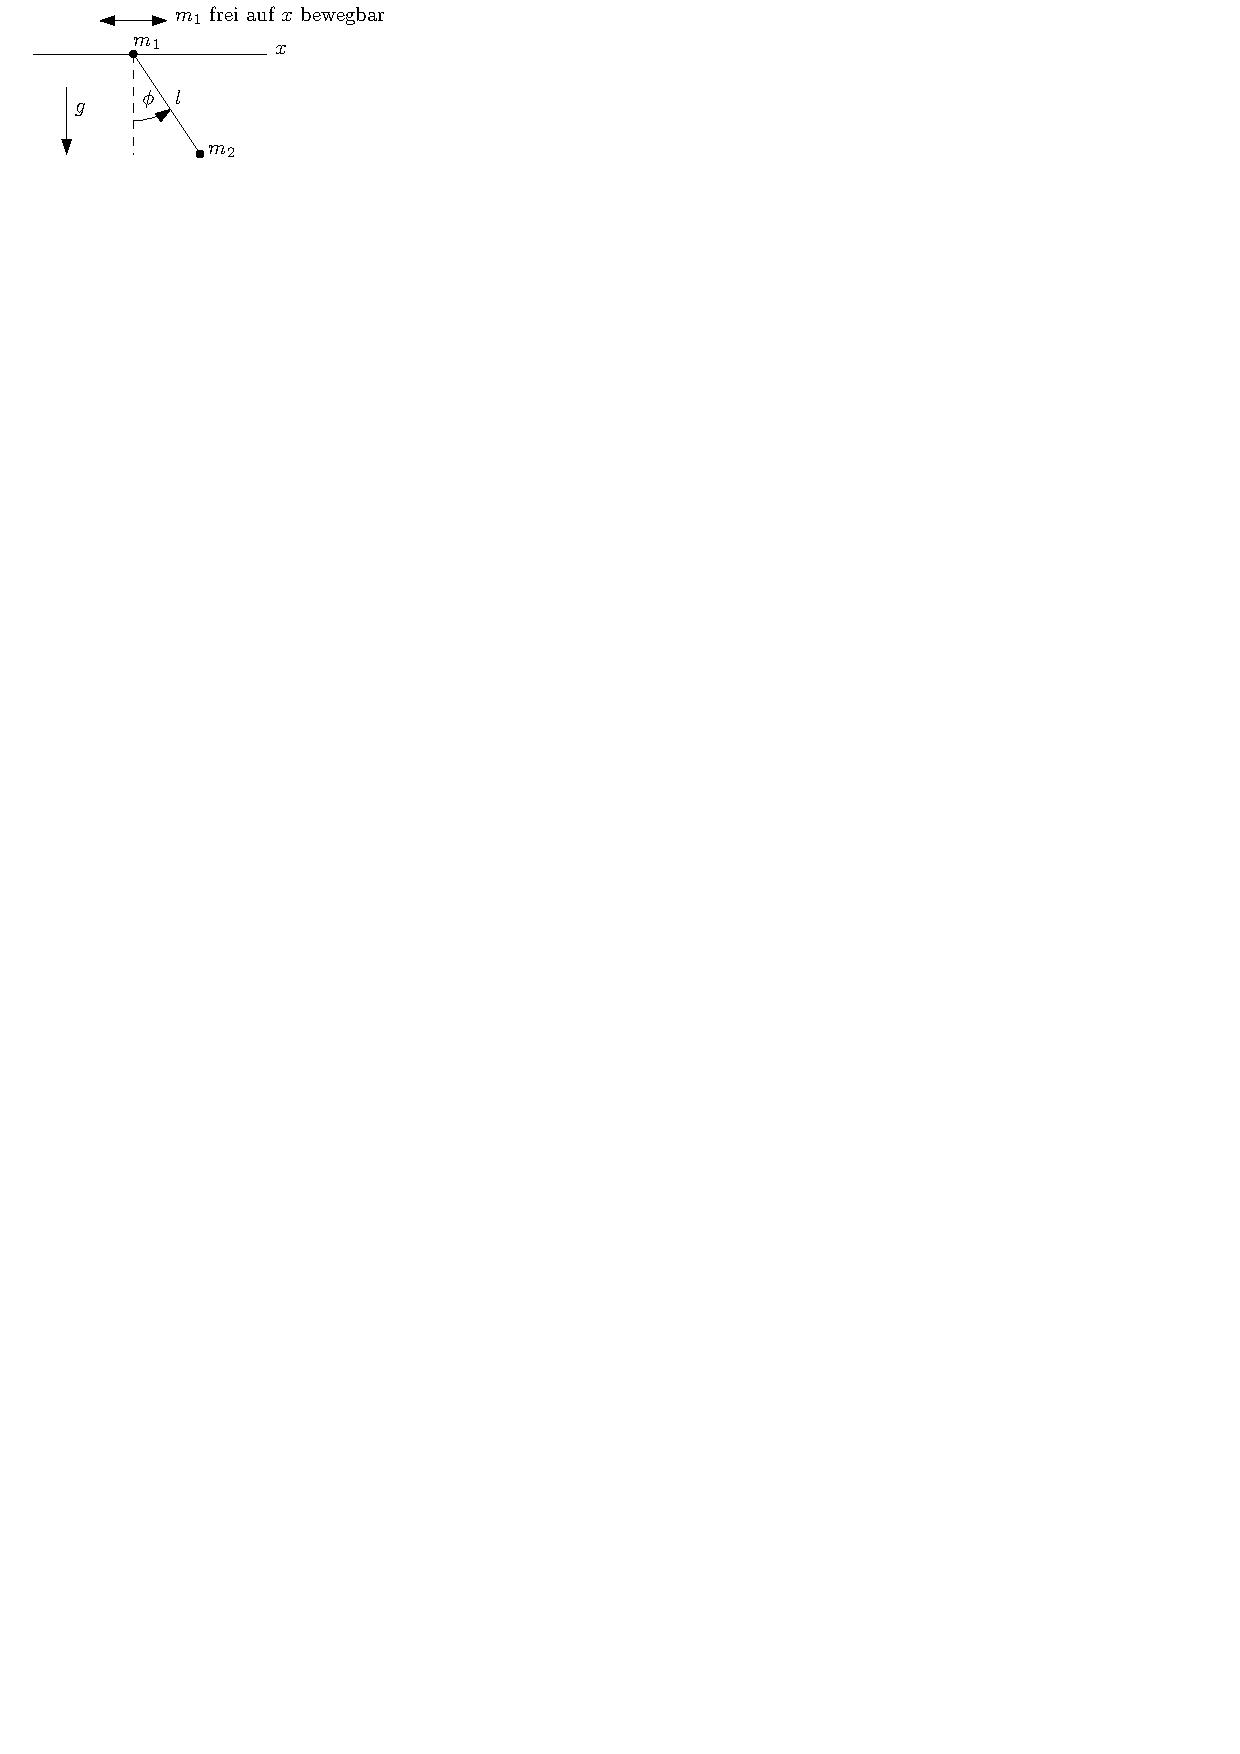
\includegraphics{figures/ch1/schwingendehantel}
		\caption{Schwingende Hantel, die an $x$-Achse aufgehängt ist. Massepunkt $m_1$ kann sich frei auf der $x$-Achse bewegen.}
		\label{fig:ch1_schwingendehantel}	
	\end{figure}

	Die Masse $m_1$ ist frei in $x$-Richtung beweglich und an der Masse $m_2$ zieht die Gravitationskraft.
	Es gibt die folgenden 4 holonom-skleronomen Zwangsbedingungen:
	\begin{align*}
	z_1 = z_2 &= 0, \\
	y_1 &= 0, \\
	(x_1 - x_2)^2 + y_2^2 - l^2 &= 0 \text{.}
	\end{align*}
	ALso gibt es im System $s = 6 - 4$ Freiheitsgrade.
	Als generalisierte Koordinaten kann man zum Beispiel $q_1 = x$ und $q_2 = \phi$ (der Winkel zwischen Lot und Hantelstange) wählen. Damit sind die Koordinaten und Geschwindigkeiten:
	\begin{align*}
	x_1 &= q_1 & x_2 &= q_1 + l \sin q_2\\
	y_1 &= 0 & y_2 &= l \cos q_2\\
	z_1 &= 0 & z_2 &= 0\\
	\dot{x}_1 &= \dot{q}_1 & \dot{x}_2 &= \dot{q}_1 + \dot{q}_2 l \cos q_2\\
	&&\dot{y}_2 &= - l \dot{q}_2 \sin q_2
	\end{align*}
	
	Schließlich folgt für die kinetische Energie:
	\begin{align*}
	T & = \frac12 m_1 \vecdotnumsq{r}{1} + \frac12 m_2 \vecdotnumsq{r}{2} \\
	&= \frac12 m_1 (\dot{x}_1^2 + \dot{y}_1^2 + \dot{z}_1^2) + \frac12 m_2 (\dot{x}_2^2 + \dot{y}_2^2 + \dot{z}_2^2) \\
	&= \frac12 m_1 \dot{q}_1^2 + \frac12 m_2 ( (\dot{q}_1 + \dot{q}_2 l \cos q_2)^2 + l^2 \dot{q}_2^2 \sin^2 q_2) \\
	&= \frac12 (m_1 + m_2) \dot{q}_1^2 + \frac12 m_2 (2 \dot{q}_1 \dot{q}_2 l \cos q_2 + \dot{q}_2^2 l^2) 
	\text{.}
	\end{align*}
	
	Mit dem Potential $V = 0 - m_2 g \cos(q_2)$ folgt die Lagrange-Funktion:
	\begin{align*}
		L &= T - V \\
		&= \frac12 (m_1 + m_2) \dot{q}_1^2 + \frac12 m_2 (l^2 \dot{q}_2^2 + 2 l \dot{q}_1 \dot{q}_2 \cos q_2) + m_2 g l \cos q_2
		\text{.}
	\end{align*}
	
	\textbf{Interessante Beobachtung}: $L$ hängt nicht von $q_1$ ab (nur von $\dot{q}_1$):
	\[
	\dd t \ffpartial{L}{\dot{q}_1} - \underbrace{\ffpartial{L}{q_1}}_{= 0} = 0
	\quad \text{und damit} \quad 	
	\ffpartial{L}{\dot{q}_1} = \text{konstant}
	\text{.}
	\]
\end{beispiel*}

\begin{definition*}[Zyklische Koordinate]\label{zyklische_koordinate}
	Ein Koordinate $q_j$ ist genau dann zyklisch falls gilt
	\[
		\ffpartial{L}{q_j} = 0 \Leftrightarrow \ffpartial{L}{\dot{q}_j} = \text{konstant} \equiv p_j
	\]
	mit dem verallgemeinerten Impuls 
	\[
		p_j = \ffpartial{L}{\dot{q_j}}
		\text{.}
	\]
	Zyklische Koordinaten führen automatisch zu einem \textit{Erhaltungssatz}. Deswegen sollten möglichst viele generalisierte Koordinaten zyklisch sein.
\end{definition*}

\begin{beispiel*}[Schwingende Hantel \textendash~Fortsetzung]
	\begin{align*}
		p_1 &= \ffpartial{L}{\dot{q}_1} = (m_1 + m_2)\dot{q}_1 + m_2 l \dot{q}_2 \cos(q_2) = \const = c'\\
		\Rightarrow \dot{q}_1 &= - \frac{m_2 l}{m_1 + m_2} \dot{q}_2 \cos(q_2) + c\\
		\overset{\text{Integration}}{\Rightarrow} q_1(t) &= ct - \frac{m_2 l}{m_1 + m_2} \sin (q_2(t))
	\end{align*}
	Die Anfangsbedingungen:
	\begin{align*}
		q_1(t = 0) &= q_2(t = 0) = 0 \\
		\dot{q}_2(t=0) &= \omega_0 \\
		\dot{q}_1(t=0) &= - \frac{m_2 l}{m_1 + m_2} \omega_0 \\
	\end{align*}
	Mit $q_1(t)$ von oben folgt $c = 0$ und wir bekommen $q_1(t) = - \frac{m_2 l}{m_1 + m_2} \sin q_2(t)$. Nun führen wir die Rücktransformation durch:

	\begin{align*}
		x_1(t) &= - \frac{m_2 l}{m_1 + m_2} \sin \phi(t), \\
		y_1(t) &= 0, \\
		x_2(t) &= - \frac{m_2 l}{m_1 + m_2} \sin \phi(t) + l \sin \phi(t) = \frac{m_1}{m_1 + m_2} l \sin \phi(t), \\
		y_2(t) &= l \cos \phi(t), \\
	\end{align*}
	wobei wir bei $x_2(t)$ die Identität $l = \frac{m_1 + m_2}{m_1 + m_2} l$ genutzt haben. Nur verwendet man die 3. Zwangsbedingung vom Anfang
	\begin{align*}
	(x_1 - x_2)^2 + y_2^2 - l^2 &= 0\\
	\Leftrightarrow \frac{(x_1 - x_2)^2}{l^2} + \frac{y_2^2}{l^2} &= 1\\ 
	\Leftrightarrow \frac{x_2^2(t)}{(\frac{m_1 l}{m_1 + m_2})^2} + \frac{y_2^2(t)}{l^2} &= 1
	\end{align*}
	Das beschreibt eine Ellipse mit den Halbachsen $\frac{m_1}{m_1 + m_2}l < l \text{~und~} l$.
	Dazu die $q_2$-Lagrange-Gleichung
	\begin{align*}
	\ffpartial{L}{\dot{q}_2} &= m_2 (l^2 \dot{q}_2 + l \dot{q}_1 \cos q_2)\\
	\dd t \ffpartial{L}{\dot{q}_2} &= m_2 (l^2 \ddot{q}_2 + l \ddot{q}_1 \cos q_2 - l \dot{q}_1 \dot{q}_2 \sin q_2)\\
	\ffpartial{L}{q_2} &= m_2 (- l \dot{q}_1 \dot{q}_2 \sin q_2 - g l \sin q_2)\\
	0 &= m_2 (l^2 \ddot{q}_2 + l \ddot{q}_1 \cos q_2 + g l \sin q_2)\\
	\intertext{Jetzt $\ddot{q}_1$ von oben (per Differentiation)}
	\ddot{q}_1 &= - \frac{m_2 l}{m_1 + m_2} (\ddot{q}_2 \cos q_2 - \dot{q}_2^2 \sin q_2)
	\end{align*}
	Damit erhält man die $q_2$-Gleichung
	\[
		l^2 \ddot{q}_2 - \frac{m_2 l^2}{m_1 + m_2}(\ddot{q_2} \cos q_2 - \dot{q}_2^2 \sin q_2) \cos q_2 + g l \sin q_2 = 0
		\text{.}
	\]
	Das ist eine nichtlineare \Dgl{} 2. Ordnung für $q_2(t) = \phi(t)$, die man vermutlich nicht per Hand lösen kann (aber numerisch). Man kann das Lösen aber durch weitere Annahmen über das System vereinfachen, zum Beispiel durch die Beschränkung auf kleine $\phi$:
	\[
		\phi(t) = \frac{\omega_0}{\omega} \sin \omega t \text{~und~} \omega = \sqrt{\frac{g}{l} \frac{m_1 + m_2}{m_1}}
		\text{.}
	\]
\end{beispiel*}


\subsubsection{Rezept für holonome Zwangsbedingungen}

Für die häufigsten Fälle mit \textbf{holonomen} Zwangsbedingungen und \textbf{konservativen} Kräften gibt es ein Rezept:
\begin{enumerate}
\item Zwangsbedingungen formulieren
\item Generalisierte Koordinaten festlegen
\item Lagrange-Funktion hinschreiben (mit generalisierten Koordinaten und Geschwindigkeiten)
\item Lagrange-Funktion ableiten und wenn möglich lösen
\item Eventuell Rücktransformation auf gewöhnliche (anschauliche) Koordinaten
\end{enumerate}

\subsubsection{Nicht-holonome Systeme}
Bei holonomen Systemen gibt es $S = 3N - p$ unabhängige generalisierte Koordinaten. Diese sind bei nicht-holonomen Systemen nicht mehr unabhängig.

Falls die nicht-holonomen Zwangsbedingungen in differentieller Form vorliegen (also als Differentialgleichung) gibt es ein Lösungsverfahren über die Methode der sogenannten Lagrange-Multiplikatoren, welche im folgenden erläutert werden.

Es gibt $\bar{p}$ Zwangsbedingungen, davon $p \leq \bar{p}$ nicht-holonom: 
\[
	i = 1, \dots, p: 
	\quad 
	\left( \sum_{m=1}^{3N} f_{im}(x_1, \dots, x_{3N}, t) \d x_m \right) + f_{it}(x_1, \dots, x_{3N}, t) \d t = 0
\]
mit $j = 3N - (\bar{p} - p)$ generalisierten Koordinaten.

Die konkreten Koordinaten hängen von den generalisierten ab: $\vec{r}_i = \vec{r}_i(\vardots{q}{j}, t)$, aber nicht alle $q_j$ sind unabhängig voneinander, wie anfangs schon erwähnt.

Damit gilt für nicht-holonome Bedingungen in $q_j$, wobei im Folgenden immer $i = 1, \dots, p$ ist:
\[
	\sum_{i=1}^j a_{im}(q_1, \dots, q_j, t) \d q_m + b_{it}(q_t, \dots, q_j, t) \d t = 0
	\text{.}
\]

Für virtuelle Verrückungen, bei denen $\delta t = 0$ gilt, ist die Gleichung wie folgt:
\[
	\sum_{m=1}^j a_{im} \delta q_m = 0
	\text{.}
\]

Nun werden die Lagrange-Multiplikatoren $\lambda_i = \lambda_i(t)$ eingeführt (nicht von $q_i$ abhängig, sondern nur von der Zeit):
\[
	\sum_{i=1}^{p} \lambda_i \sum_{m=1}^j a_{im} \delta q_m = 0
	\text{.}
\]
Bei konservativen Systemen (siehe oben) gilt mit dem Prinzip von d'Alembert:
\[
	\sum_{m=1}^j \left( \ffpartial{L}{q_m} - \dd t \ffpartial{L}{\dot{q}_m} \right) \delta q_m = 0
\]

Wobei diese Gleichung nur als Summe gültig ist, da die $\delta q_m$ nicht mehr unabhängig voneinander sind. Zusammengefasst folgt
\[
	\sum_{m=1}^j \left( \ffpartial{L}{q_m} - \dd t \ffpartial{L}{\dot{q}_m} + \sum_{i=1}^p \lambda_i a_{im} \right) \delta q_m = 0
	\text{.}
\]

Nur ein Teil der generalisierten Koordinaten ist, wie schon oft erwähnt, unabhängig voneinander: $m = 1, \dots, j - p$ sind unabhängig und $m = j - p + 1, \dots j$ (genau $p$ Bedingungen) sind abhängig, die Wahl der $q_m$ findet dementsprechend statt.

Wähle für die letzten $p$ Gleichungen die bisher nicht bestimmten $\lambda_i$ so, dass
\[
	m = j-p+1, \dots, j: 
	\quad 
	\ffpartial{L}{q_m} - \dd t \ffpartial{L}{\dot{q}_m} + \sum_{i=1}^p \lambda_i a_{im} = 0
	\text{.}
\]
Das geht, da es $p$ Gleichungen und genauso viele $\lambda_i$'s gibt. Damit hat man nur noch Gleichungen mit unabhängigen $q_m$, also
\[
	\sum^{j - p}_{m = 1} \left( \ffpartial{L}{q_m} - \dd t \ffpartial{L}{\dot{q}_m} + \sum^p_{i = 1} \lambda_i a_{im} \right) \delta_{q_m} = 0
	\text{.}
\]
Hier kann man die $\delta_{q_m}$ unabhängig variieren, also jeder Summand $=0$. Daraus entstehen Lagrange-Gleichungen 1. Art entstehen für alle $m$:
\[
	m = 1, \dots, j:
	\quad
	\dd t \ffpartial{L}{\dot{q}_m} - \ffpartial{L}{q_m} = \sum_{i=1}^p \lambda_i a_{im}
	\text{.}
\]
Hierbei gilt noch $\sum_{m=1}^j a_{im} \dot{q}_m + b_{it} = 0$ für $i = 1, \dots, p$. Damit hat man $j + p$ Gleichungen für $j$ generalisierte Koordinaten und $p$ Multiplikatoren $\lambda_i$.

Ein Vergleich mit den generalisierten Kräften zeigt $\bar{Q}_m = \sum_{i=1}^{p} \lambda_i a_{im}$.
Nun hat man generalisierte Zwangskräfte ($\sum_{m=1}^j \bar{Q}_m \delta q_m = 0$) was den $\lambda_i$ entspricht.
Dieses Wissen ist auch ein Gewinn für Systeme mit holonomen Zwangsbedingungen, denn die Kenntnis der Zwangskräfte ist nützlich für das Design des Systems.

\textbf{Anwendung auf holonome Systeme}: 
$f_i(\vardots{\vec{r}}{N}, t) = 0, i = 1, \dots, p$ in generalisierten Koordinaten $\bar{f}_i(\vardots{q}{j}, t) = 0$, daraus folgt das totale Differential 
\[
	\d \bar{f}_i = \sum_{m=1}^j \ffpartial{\bar{f}_i}{q_m} \d q_m + \ffpartial{\bar{f}_i}{t} \d t
\]
und damit ($\d \bar{f}_i = 0$ für $i = 1, \dots, p$)
\[
	a_{im} = \ffpartial{\bar{f}_i}{q_m}
	\quad \text{sowie} \quad
	b_{it} = \ffpartial{\bar{f}_i}{t}
	\text{.}
\]
Die Zwangskräfte in holonomen Systemen können nun mit Lagrange-Gleichungen 1. Art bestimmt werden.

\begin{beispiel*}[holonome Zwangsbedingungen mit Zwangskräften]
Es wird ein Pendel mit Winkel $\varphi$ zum Lot, der Länge $l$ und der Masse $m$ betrachtet (siehe Abbildung \ref{fig:ch1_fadenpendel}).
\begin{figure}
	\centering
	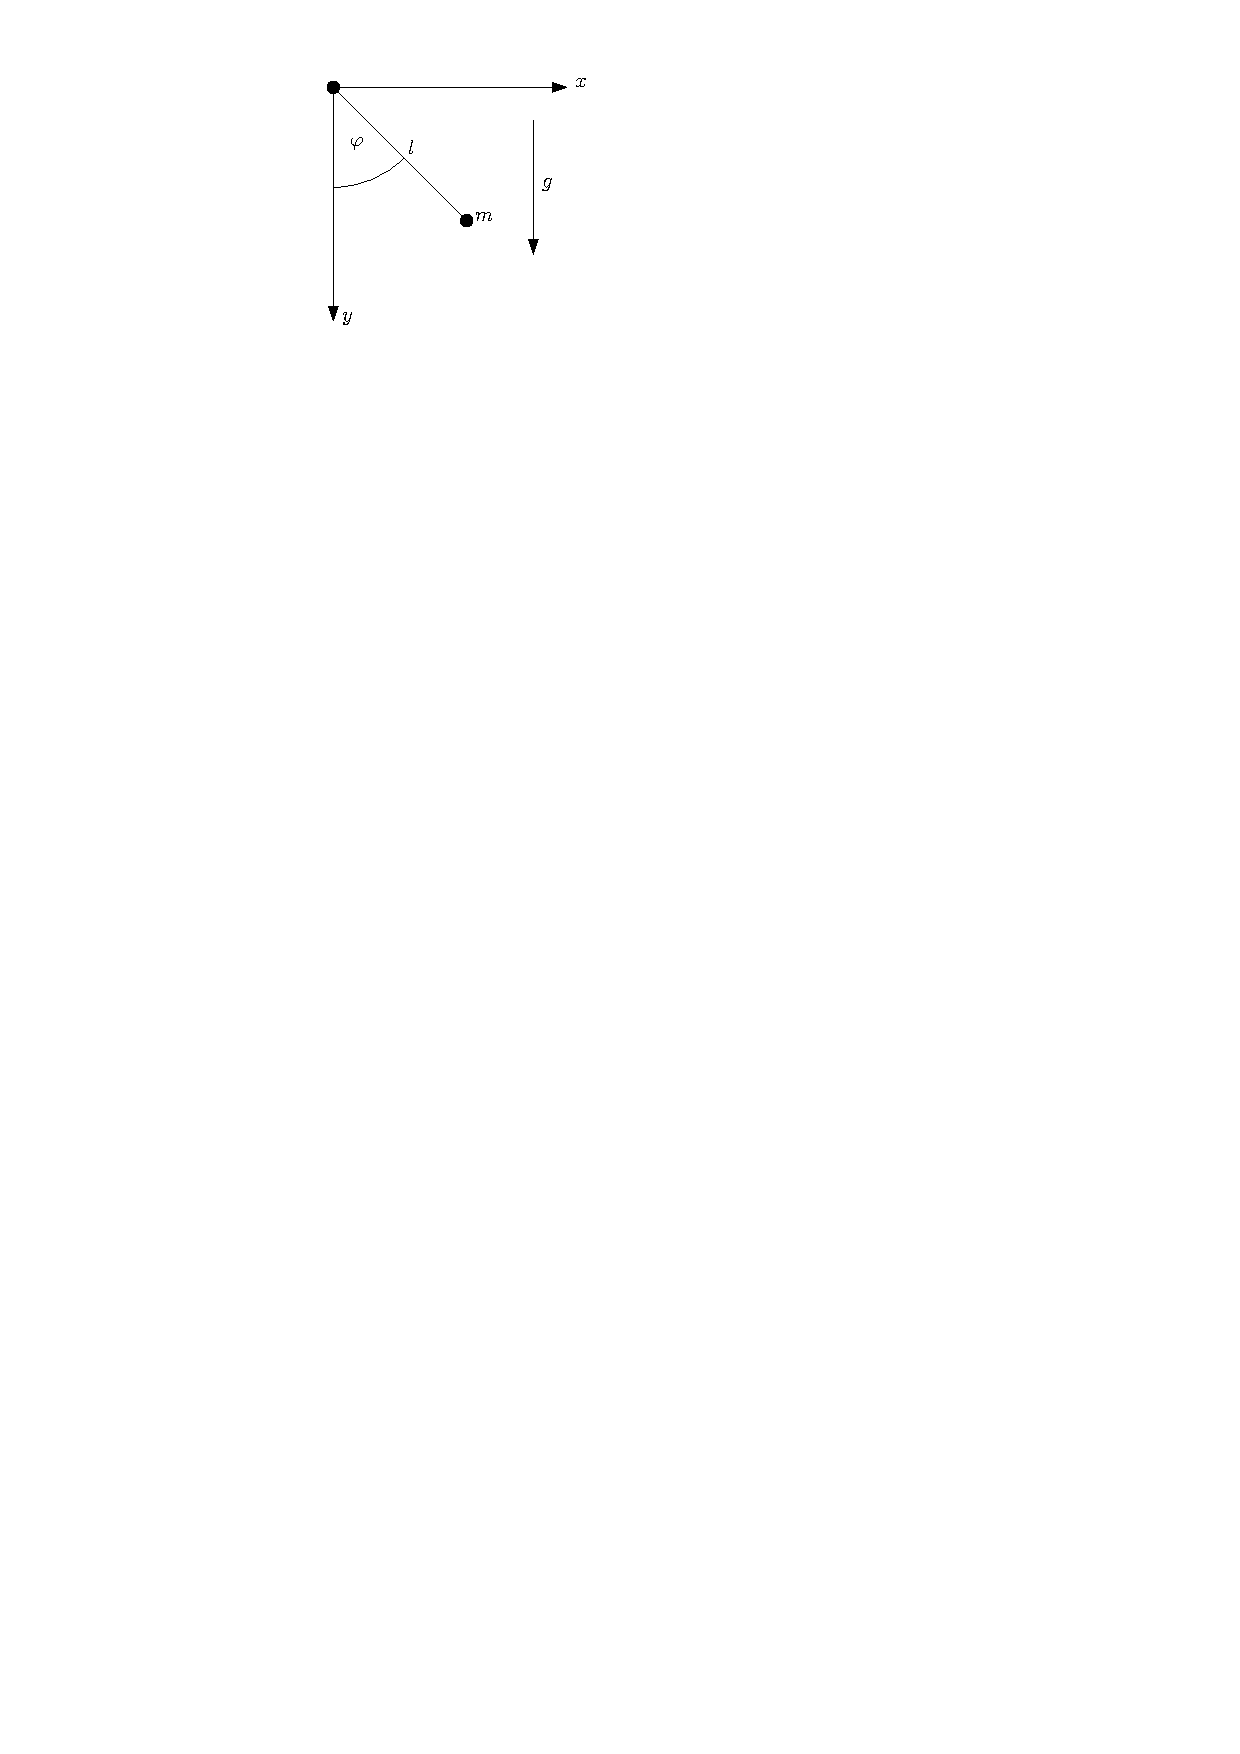
\includegraphics{figures/ch1/fadenpendel}
	\caption{Ein Fadenpendel der Masse $m$.}
	\label{fig:ch1_fadenpendel}
\end{figure}
Zunächst wird $r=l$ variabel gewählt. Die verallgemeinerten Koordinaten sind deswegen $\varphi$ und $r$.
\begin{align*}
x &= r \sin \varphi\\
y &= l - r \cos \varphi\\
f(x,y,t) &= r - l = 0 \text{~~~~ist die Zwangsbedingung}\\
V &= -mg y = -mg (l -r \cos \varphi)\\
T &= \frac12 m (\dot{x}^2 + \dot{y}^2)\\
\dot{x} &= \dot{r} \sin \varphi + r \dot{\varphi} \cos \varphi\\
\dot{y} &= - \dot{r} \cos \varphi + r \dot{\varphi} \sin \varphi\\
\dot{x}^2 + \dot{y}^2 &= \dot{r}^2 \sin^2 \varphi + 2 r \dot{r} \dot\varphi \sin \varphi \cos \varphi \\
&+ r^2 \dot{\varphi}^2 \cos^2 \varphi + \dot{r}^2 \cos^2 \varphi - 2 r \dot r \dot \varphi \sin \varphi \cos \varphi + r^2 \dot{\varphi}^2 \sin^2 \varphi \\
&= \dot{r}^2 + r^2 \dot{\varphi}^2\\
L &= T-V = \frac12 m (\dot{r}^2 + r^2 \dot{\varphi}^2) + mg(l - r \cos \varphi)\\
\ffpartial{L}{r} - \dd t \ffpartial{L}{\dot{r}} &= m r \dot{\varphi}^2 - mg \cos \varphi - \dd t m \dot{r} \\
&= -m (g \cos \varphi + \ddot{r} - r \dot{\varphi}^2)\\
\ffpartial{L}{\varphi} - \dd t \ffpartial{L}{\dot{\varphi}} &= mgr \sin \varphi - \dd t m r^2 \dot{q} \\
&= mgr \sin \varphi - 2mr\dot{r}\dot{\varphi} - mr^2 \ddot{\varphi}\\
\end{align*}
Zwangsbedingung $r-l = 0 = \bar{f}(r, \varphi, t)$\\
$\ffpartial{f}{r} = 1$ alle anderen partiellen Ableitungen $= 0$\\
\conseq $\lambda_r = \bar{Q}_r$ ist Zwangskraft in $r$-Richtung

Daraus folgen die drei Gleichungen:
\begin{itemize}
	\item \textbf{$r$-Gleichung}: $\lambda = m \ddot{r} + mg \cos \varphi - m r \dot{\varphi}^2$,
	\item \textbf{$\varphi$-Gleichung}: $\ddot{\varphi} + \frac{2 \dot{r}}{r} \dot{\varphi} + \frac{g}{r} \sin \varphi = 0$ und
	\item \textbf{$l$-Gleichung}: $r = l \rightarrow \dot{r} = \ddot{r} = 0$.
\end{itemize}
Randbemerkung: $\lambda = -m(l \dot{\varphi}^2 - g \cos \varphi)$ ist hier die Fadenspannung.

Das ganze kann man vereinfachen wenn man $\dot{r} = 0$ und $\sin \varphi \approx \varphi$ annimmt (letzteres gilt für kleine $\varphi$). Damit gilt dann folgendes ($\ddot{\vp} + \frac{g}{l} \vp = 0$)
$$\varphi(t) = \varphi_0 \sin \sqrt{\frac{g}{l}} t$$
\end{beispiel*}

\subsection{Das Hamiltonsche Prinzip}	
Wir zeigen, dass die Lagrange-Gleichungen nicht nur aus dem differentiellen Prinzip von d'Alembert folgen: gerade hatten wir momentane virtuelle Verrückungen betrachtet.
\textbf{Dagegen Hamilton}: \textbf{Integralprinzip}\\
Das ist die Variation der gesamten Bahn bei festen Endpunkten.
Dazu betrachten wir Bahnen $\vec{q}(t)$ im Konfigurationsraum
$$\vec{q}(t) = (q_1(t), \dots, q_s(t))$$
ein $\vec{q}(t)$ beschreibt einen Zustand des gesamten Systems. Für gegebene $\vec{q}(t)$ und $\dot{\vec{q}}(t)$ wird die Lagrange-Funktion eine Funktion der Zeit 
$$L(\vec{q}(t), \dotvec{q}(t), t) = \tilde{L}(t)$$

\begin{definition*}[Wirkungsfunktional]
$$S\{\vec{q}(t)\} = \int_{t_1}^{t_2} \tilde{L}(t) \d t$$
Die Dimension hiervon ist "`Wirkung"' \conseq Energie:
$S$ hängt von $\vec{q}(t)$ und $t_1, t_2$ ab. 
Funktion $\vec{q}(t) \xrightarrow{\text{Abbildung}} S \{ \vec{q}(t) \}$ im allgemeinen Funktional.

Wir betrachten Scharen $\vec{q}(t)$ mit den gleichen Endpunkten $\vec{q}(t_1)$ und $\vec{q}(t_2)$. Virtuelle Verrückungen müssen verschwinden.	
\end{definition*}


Beim Hamiltonschen Prinzip wird nun die Bahn des Systems betrachtet und wir wollen eine extremale Bahn finden.

~\\
\begin{definition*}[Hamiltonsches Prinzip]
Die Systembewegung erfolgt so, dass $S\{\vec{q}(t)\}$ für die richtige Trajektorie extremal wird, d.h. dass die Variation bezüglich der tatsächlichen Bahn verschwindet.
$$\delta S = \delta \int_{t_1}^{t_2} L(\vec{q}(t), \dotvec{q}(t), t) \d t \overset{!}{=} 0$$
\end{definition*}

\begin{bemerkung*}
	Die Gleichung $\delta S = 0$ enthält auf elegante Weise die gesamte klassische Mechanik. Das Prinzip (der Minimierung der Trajektorie) wird auch jenseits der Mechanik verwendet\footnote{Zum Beispiel in der Teilchenphysik, der geometrischen Optik (Fermatsches Prinzip, dabei bewegt sich Licht auf einer Bahn, so dass die benötigte Zeit minimal ist. Damit können die Brechungsindizes gefunden werden.)}. Es ist natürlich koordinatenunabhängig.
\end{bemerkung*}

\begin{bemerkung*}
	Das Hamiltonsche Prinzip wird auch jenseits der klassischen Mechanik verwendet. Beispielsweise in der Teilchenphysik (Quantenfeldtheorie) oder in der Optik.
\end{bemerkung*}

\subsubsection{Äquivalenz zum Prinzip von d'Alembert}
\begin{align*}
\sum_{i=1}^N (m_i \ddotvec{r}_i - \vec{K}_i) \delta \vec{r_i} &= 0\\
\intertext{Integration über die Zeit}
\int_{t_1}^{t_2} (\sum_{i=1}^N (m_i \ddotvec{r}_i - \vec{K}_i) \delta \vec{r_i}) \d t &= 0
\intertext{mit $\ddotvec{r}_i \delta \vec{r}_i = \dd t (\dotvec{r}_i \cdot \delta \vec{r}_i) - \dotvec{r}_i \cdot \delta \dotvec{r}_i = \dd t (\dotvec{r}_i \cdot \delta \vec{r}_i) - \frac12 \delta \dot{(\vec{\hspace{-1em}r\hspace{1em}}_i^2)}$}
\int_{t_1}^{t_2} (\sum_{i=1}^N (\dd t (m_i \dotvec{r}_i \cdot \vec{r}_i) - \frac12 m_i \delta (\dotvec{r}_i^2) - \vec{K}_i \cdot \delta \vec{r}_i) \d t &= 0
\intertext{Integration}
\int_{t_1}^{t_2} \sum_{i=1}^N \dd t (m_i \dotvec{r}_i \cdot \delta \vec{r}_i) \d t
=  \left. \sum_{i=1}^N m_i \dotvec{r}_i \cdot \delta \vec{r}_i \right|_{t_1}^{t_2} &= 0\\
\intertext{Keine Variation an den Endpunkten}
\Rightarrow \int_{t_1}^{t_2} \sum_{i=1}^N [ \delta (\frac{m_i}{2} \dotvec{r}_i^2 ) + \vec{K}_i \cdot \delta \vec{r}_i ] \d t &= 0
\intertext{mit $\vec{r}_i = \vec{r}_i(q_1, \dots, q_s, t)$, $i = 1, \dots, N$ findet man die generalisierte Kraft und das konservative Potential mit holonomen Zwangsbedigungen.}
\sum_{i=1}^N \vec{K}_i \delta \vec{r}_i = \sum_{j=1}^s Q_j \delta q_j = \sum_{j=1}^{s} - \ffpartial{V}{q_j} \delta q_j &= - \delta V
\intertext{Daraus folgt dann zusammen genommen die Äquivalenz des Prinzips von d'Alembert und dem Hamiltonschen}
0 = \int_{t_1}^{t_2} \delta (T-V) \d t = \delta \int_{t_1}^{t_2} (T-V) \d t = \delta \int_{t_1}^{t_2} L \d t &= 0
\end{align*}

Bewegungsgleichungen? \conseq Variationsrechnung.
Finden der Kurve $\vec{q}(t)$, die $S\{\vec{q}(t)\}$ extremal macht.

\subsubsection{Elemente der Variationsrechnung}

\begin{definition*}[Euler-Gleichung]
	Sie ist aufgebaut wie die Lagrange-Gleichung, gilt aber ganz allgemein für Variationsprobleme.
	$$ \ffpartial{f}{y} - \dd x \ffpartial{f}{y'} = 0$$
\end{definition*}~\\
Zunächst ein eindimensionales Problem.
\paragraph{Problem} Finde eine Kurve $y(x)$ für die ein bestimmtes Funktional extremal wird. Zum Beispiel "`eine kürzeste Verbindung"', beispielsweise auf einer krummen Fläche (Geodäte) wie einer Seifenhaut.
Die verschiedenen möglichen Verbindungen bilden eine Schar $f(x, y, y')$ von $y(x)$ mit festen Endpunkten. Es wird angenommen, dass $f$ differenzierbar in allen Variablen ist. Im folgenden gilt weiterhin $y' = \ddd{y}{x}$.
Wir bilden das Funktional
\begin{align*}
J\{y(x)\} &= \int_{x_1}^{x_2} f(x, y, y') \d x = \int_{x_1}^{x_2} \tilde{f}(x) \d x
\end{align*}
Das Problem kann nun wie folgt ausgedrückt werden: Für welches $y(x)$ wird $J\{y(x)\}$ extremal?\\
Dies ist ähnlich zu einer einfachen Extremwertaufgabe, wenn die Schar $y(x)$ durch den Parameter $\alpha$ parametrisiert werden kann. Dies kann zum Beispiel so geschehen, dass
\begin{align*}
y_{\alpha = 0}(x) &= y_0(x)
\intertext{die extremale und damit gesuchte Bahn wird. Damit kann man jetzt $y_\alpha$ aufteilen}
y_\alpha(x) &= y_0(x) + \gamma_\alpha(x)
\intertext{$\gamma_\alpha(x)$ ist hierbei eine fast beliebige, differenzierbare Funktion, welche an den Endpunkten für alle $\alpha$ verschwindet, also 0 wird. Nach dem, wie $\gamma_\alpha$ konstruiert wurde gilt auch}
\gamma_{\alpha = 0}(x) &= 0~~~\forall x
\intertext{Man kann $\gamma_\alpha$ auch anders angeben: $\gamma_\alpha(x) = \alpha \eta(x), ~~~ \eta(x_1) = \eta(x_2) = 0$. $x$ wird festgehalten und dann eine Taylorreihe mit $\alpha = 0$ wie folgt entwickelt}
\gamma_\alpha(x) &= \alpha (\ffpartial{\gamma_\alpha(x)}{\alpha})_{\alpha = 0} + \frac{\alpha^2}{2} (\frac{\partial^2 \gamma_\alpha(x)}{\partial \alpha^2})_{\alpha = 0} + \dots
\intertext{Oder wieder anders}
\gamma_\alpha(x) &= y_0(x) + \alpha(\ffpartial{y_\alpha}{\alpha})_{\alpha = 0} + \dots
\end{align*}

$y_\alpha(x)$ wird nun in der Nähe (besser gesagt in der $\epsilon$-Umgebung) von $\alpha = 0$ variiert. Daraus folgt, dass $\alpha \rightarrow \d \alpha$.
Und damit $\delta y = y_{\d \alpha} - y_0(x) = \d \alpha (\ffpartial{y_\alpha(x)}{\alpha})_{\alpha = 0}$.
Wird nun $\delta y$ bei festem $x$ betrachtet (vgl. virtuelle Verrückungen bei fester Zeit t. ($\delta t = 0$)) kommt man zu einer Variation des Funktionals $J\{y(x)\}$
\begin{align*}
\delta J &= J \{ y_{\d \alpha}(x) \} - J\{ y_0(x)\} = (\ddd{J(x)}{\alpha})_{\alpha = 0} \d \alpha\\
&= \int_{x_1}^{x_2} (f(x, y_{\d \alpha}, y'_{\d \alpha}) - f(x, y_0, y'_0)) \d x
\end{align*}
Jetzt ist die Extremalbedingung offensichtlich: Es muss für beliebige $\gamma_{\alpha}(x)$ gelten
$$(\ddd{J(\alpha)}{\alpha})_{\alpha = 0} = 0$$
Damit ist $y_0(x)$ eingesetzt ist die gesuchte Bahn. Es ist eine stationäre Bahn genau dann, wenn $\delta J \overset{!}{=} 0$.
Durch einfaches Umformen folgt damit
\begin{align*}
(\ddd{J(\alpha)}{\alpha}) &= \int_{x_1}^{x_2} \d x (\ffpartial{f}{y} \ffpartial{y}{\alpha} + \ffpartial{f}{y'} \ffpartial{y'}{\alpha} + \ffpartial{f}{x} \ffpartial{x}{\alpha})
\intertext{mit der Identität $\int_{x_1}^{x_2} \d x \ffpartial{f}{y'} \ffpartial{y'}{\alpha} = \int_{x_1}^{x_2} \d x \ffpartial{f}{y'} \dd x \ffpartial{y}{\alpha}$, $\ffpartial{y'}{\alpha} = \fpartial{\alpha} \ddd{y}{x} = \dd x \ffpartial{y}{\alpha}$ und partieller Integration folgt}
&= \underbrace{\left. \ffpartial{f}{y'} \ffpartial{y}{\alpha} \right|_{x_1}^{x_2}}_{\hspace{-10em}=0, \text{~da keine Variation an den Endpunkten.\hspace{-10em}}} - \int_{x_1}^{x_2} \d x (\dd x \ffpartial{f}{y'}) \ffpartial{y}{\alpha}\\
\dd \alpha J(x) &= \int_{x_1}^{x_2} \d x (\ffpartial{f}{y} - \dd x \ffpartial{f}{y'}) \ffpartial{y}{\alpha}\\
\delta J &= \int_{x_1}^{x_2} \d x (\ffpartial{f}{y} - \dd x \ffpartial{f}{y'}) \delta y
\end{align*}
$\delta J \overset{!}{=} 0$ für beliebige $\delta y$ damit verschwindet der Integrand. Daraus folgt wieder die Eulersche Gleichung
$$\ffpartial{f}{y} - \dd x \ffpartial{f}{y'} = 0$$
Und damit eine Differentialgleichung 2. Ordnung für das gesuchte $y(x)$. (vgl. Lagrange-Gleichung 2. Art)

\begin{beispiel*}[Kürzeste Verbindung zweier Punkte in der Ebene]~\\
	Welches Funktional? (Infinitesimale Länge $\d s = \sqrt{\d x^2 + \d y^2}$) Gesucht ist $\int_{p_1}^{p_2} \d s = J$\\
	$$J = \int_{p_1}^{p_2} \d s = \int_{x_1}^{x_2} \sqrt{\d x^2 + \d y^2} = \int_{x_1}^{x_2} \sqrt{1 + (\ddd{y}{x})^2} \d x = \int_{x_1}^{x_2} \sqrt{1 + {y'}^2} \d x$$
	$\delta J = 0$ führt zur extremalen Bahn $y(x)$. 
	$$ f(x, y, y') = \sqrt{1 + {y'}^2}$$
	Nun verwenden wir die Euler-Gleichung: $\ffpartial{f}{y} = 0$; $\ffpartial{f}{y'} = \frac{y'}{\sqrt{1 + {y'}^2}}$ und damit folgt
	$$\dd x \frac{y'}{\sqrt{1 + {y'}^2}} = 0$$
	oder anders gesagt
	$$\frac{y'}{\sqrt{1 + {y'}^2}} = \text{konstant} = c \qquad \Rightarrow \qquad {y'}^2 = c^2 ( 1 + {y'}^2)$$
	Zusammenfassend folgt damit mit ${y'}^2(1 - c^2) = 1$, dass $y'$ konstant ist
	und damit schlussendlich auch die Lösung des Problems
	$$y(x) = a x + b$$
	$a$, $b$ werden über die Anfangsbedingungen$(x_1, y_1)$ und $(x_2, y_2)$ festgelegt.
\end{beispiel*}

\begin{beispiel*}[Minimale Rotationsfläche]~\\
Die Punkte $(x_1,y_1),(x_2,y_2)$ rotieren um die $y$-Achse. Gesucht ist die Kurve zwischen ihnen, welche die Rotationsfläche minimiert. (Seifenblasen-Verhalten.)
\textit{Es wird im Grunde genommen wie beim letzten Beispiel vorgegangen.} Die Minimalfläche ist
\begin{align*}
J &= \int \d A = \int 2 \pi x \d s
\intertext{mit $\d s = \sqrt{\d x^2 + \d y^2} = \sqrt{1 + (\ddd{y}{x})^2} \d x = \sqrt{1 + {y'}^2} \d x$ folgt}
&= 2 \pi \int_{x_1}^{x_2} x \sqrt{1 + {y'}^2} \d x
\end{align*}
Wenn $\delta J = 0$ gilt, ist $J$ die extremale Fläche, d.h. die minimalgroße Fläche.
Es wird nun die Funktion, besser gesagt die Variation, $f$ definiert 
\begin{align*}
f(x,y,y') &= x \sqrt{1 + {y'}^2} & \text{~\textit{mit }}y' = \ddd{y}{x}\\
\ffpartial{f}{y} &= 0 & \ffpartial{f}{y'} = \frac{x y'}{\sqrt{1 + {y'}^2}}\\
\xRightarrow[]{\text{Eulergleichung}} \dd x \frac{x y'}{\sqrt{1 + {y'}^2}} &= 0\\
\frac{x y'}{\sqrt{1 + {y'}^2}} &= \text{konstant} = a\\
\ddd{y}{x} &= y' = \frac{a}{\sqrt{x^2 - a^2}}\\
y(x) &= a \arcosh (\frac{x}{a}) + b & \text{~\textit{oder }} x(y) = a \cosh (\frac{y - b}{a})
\end{align*}
$a$, $b$ können wieder mithilfe der Anfangsbedingungen $(x_1, y_1)$ und $(x_2, y_2)$ gefunden werden.\\
Ein Hinweis am Rande: Die Kurve, welche durch den Kosinus Hyperbolicus beschrieben wird, wird auch Kettenlinie\footnote{\href{https://de.wikipedia.org/wiki/Kettenlinie_\%28Mathematik\%29}{Wikipedia}} genannt.
\end{beispiel*}

\subsubsection{Verallgemeinerung des Variationsproblems auf mehrere Variablen}
\textit{\dots und damit die Euler-Gleichung natürlich auch.}\\
Das betrachtete $y$ wird nun als Vektor $\vec{y}(x) = (y_1(x), \dots, y_s(x))$ geschrieben und ganz analog gilt
$$\delta J = \int_{x_1}^{x_2} \d x \sum_{i=1}^{s} (\ffpartial{f}{y_i} - \dd x \ffpartial{f}{y'_i}) \delta y_i = 0$$
Hierbei sind $\delta y_i$ die unabhängigen Freiheitsgrade. Offensichtlich gibt es eine Gleichung pro Freiheitsgrad
\begin{align*}
\ffpartial{f}{y_i} - \dd x \ffpartial{f}{y'_i} &= 0, i = 1, \dots, s
\intertext{Dies stellt in etwa die Euler-Lagrange-Gleichungen dar. Nun kann man das Hamiltonsche Prinzip anwenden}
\delta \int L(t, \vec{q}, \dotvec{q}) \d t &\overset{!}{=} 0
\intertext{Es funktioniert also völlig analog. Damit bekommt man Lagrange-Gleichungen 2. Art}
\dd t \ffpartial{L}{\dot{q}_i} - \ffpartial{L}{q_i} &= 0
\end{align*}
\conseq \textbf{Hamiltonsches Prinzip}
Das Integralprinzip (Hamilton) und das differentielle Prinzip (d'Alembert) sind äquivalent. Beide führen auf die Lagrange-Gleichungen. 

\textit{Das Hamiltonsche Prinzip wird ausgiebig in der Quantenmechanik verwendet. Im folgenden wird weiter auf die Hamilton-Funktion eingegangen um als Ziel sich in die Quantenmechanik zu bewegen. Es werden im speziellen Eigenschaften der Hamilton-Funktion angegeben.}

\subsubsection{Erhaltungsgrößen}
\paragraph{Allgemeines System} Die allgemeinen Koordinaten $q_i$, $\dot{q}_i$ für $i = 1, \dots, s$ sind im Laufe der Zeit veränderlich, womit es $2S$ Funktionen der Zeit gibt. Einige von diesen sind jedoch konstant\footnote{Mathematisch ausgedrückt gilt dann $F_r = F_r(q_1, \dots, q_s, \dot{q}_1, \dots, \dot{q}_s, t) = \text{konstant}$.}, was nicht Zufall sein muss.\footnote{Es ist aus offensichtlichen das Ziel, dass möglichst viele Funktionen konstant sind. Denn wie man schon im Lagrange-Teil gesehen hat, wird damit die Komplexität des Problems reduziert.}
Diese konstanten Funktionen heißen auch \textbf{Integrale der Bewegung}.

\paragraph{Im Prinzip gilt} Bei $2S$ Integralen der Bewegung $C_i$ ist das Problem gelöst, weil $q_i = q_i(C_1, \dots, C_{2S}, t)$ und damit das Problem nicht mehr dynamisch ist. Die Lösung kann dann einfach abgelesen werden.

Einige Konstanten der Bewegung hängen mit den Grundeigenschaften von Raum und Zeit zusammen (siehe unten).

Allgemein gilt, dass, wie schon gesagt, möglichst viele Konstanten der Bewegung bestimmt werden sollten, bevor die Lösung angestrebt wird. Einige der möglichen Konstanten haben wir schon kennengelernt: Die Resultate zyklischer Koordinaten: $q_i$ sei zyklisch\footnote{vgl. \ref{zyklische_koordinate}}, damit gilt
$$p_j = \ffpartial{L}{\dot{q}_j} = \text{konstant}$$
Ein gutes Beispiel hierfür sind Zweikörperprobleme.

\begin{beispiel*}[Zweikörperproblem\footnote{\href{http://de.wikipedia.org/wiki/Zweik\%C3\%B6rperproblem}{Wikipedia}}\footnote{Konkrete Beispiele sind die Anziehung zwischen Protonen und Elektronen im Atom oder jener zwischen Sonne und Erde.}]~\\
Zwei Massepunkte $m_1$ und $m_2$ haben die Koordinaten $\vec{r}_1$ und $\vec{r}_2$ und die Relativkoordinate $\vec{r} = \vec{r}_i - \vec{r}_2$. Als Kraft herrscht nur das Potentialfeld\footnote{Nur abhängig von der relativen Position der Massepunkte. Beispiele hierfür sind das Gravitationsfeld oder das elektrische Feld}
\begin{align*}
V(\vec{r}_1, \vec{r}_2) &= V(| \vec{r}_1 - \vec{r}_2|) = V(r)\\
\text{Gesamtmasse~~~} M &= m_1 + m_2\\
\text{reduzierte Masse~~~} \mu &= \frac{m_1 m_2}{m_1 + m_2}\\
\text{Schwerpunkt~~~} R &= \frac{1}{M} (m_1 \vec{r}_1 + m_2 \vec{r}_2)\\
\text{Relativkoordinate~~~} \vec{r} &= \vec{r}_1 - \vec{r}_2 = r (\sin \vartheta \cos \varphi, \sin \vartheta \sin \varphi, \cos \vartheta)
\end{align*}~\\
\emph{Wir Erwarten}
\dots das sowohl die Bewegung des Schwerpunkts trivial, also gleichförmig, ist wie auch die Bewegung der reduzierten Masse $\mu$ im Schwerpunktsystem ist.\\~\\
Die generalisierten Koordinaten sind in unserem Beispiel
\begin{align*}
\vec{R} &= (q_1, q_2, q_3) \text{~mit~} r = q_4, \vartheta = q_5, \varphi = q_6
\intertext{Damit ist die Lagrange-Funktion in den generalisierten Koordinaten}
	L &= \frac{M}{2} (\dot{q}_1^2 + \dot{q}_2^2 + \dot{q}_3^2) \\~&- V(q_4) + \frac{\mu}{2} (\dot{q}_4^2 + q_4^2 \dot{q}_5^2 + q_4^2 \dot{q}_6^2 \sin^2 q_5)
	\intertext{Offensichtlich sind die Koordinaten $q_1, q_2, q_3, q_6$ zyklisch und $p_i = \ffpartial{L}{\dot{q}_i} = M \dot{q}_i$ für ($i =1, 2, 3$), also bleibt der \textit{Schwerpunktimpuls} erhalten.}
	\vec{p} &= M \dotvec{R} = \text{konstant}\\
	p_6 &= \ffpartial{L}{\dot{q}_6} = \mu q_4^2 \dot{q}_6 \sin^2 q_5 = \mu \dot{\varphi} r^2 \sin^2 \vartheta = L_r^{(Z)} = \text{konstant}
\end{align*}
Die $z$-Komponente des Relativdrehimpulses ist offensichtlich konstant\footnote{Vergleiche: Geworfenes Frisbee, dessen Drehachse relativ gesehen sich nicht verändert.\footnote{Tipp: Dies mit einer Tafelkreide zu probieren ist aufgrund des vergleichsweise geringen Impulses schlecht möglich.}}.
Wenn man nun versucht das Problem in den Kartesischen Koordinaten anzugehen, führt das zu folgender Lagrange-Funktion:
\begin{align*}
	L =& \frac{m_1}{2} (\dot{x}_1^2 + \dot{y}_1^2 + \dot{z}_1^2) + \frac12 m_2 (\dot{x}_2^2 + \dot{y}_2^2 + \dot{z}_2^2) \\
	&- V((x_1 - x_2)^2 + (y_1 - y_2)^2 + (z_1 - z_2)^2)
	\intertext{Auch hier sind die Erhaltungssätze gültig. Sie sind aber viel schwerer abzulesen.}
\end{align*}
\end{beispiel*}

\subsubsection{Homogenität in der Zeit}
Das bedeutet die Invarianz der Bewegung gegenüber Zeittranslationen\footnote{Das gleiche zu einem späteren Zeitpunkt starten.}\footnote{Der Informatiker kennt das auch als seiteneffektfreie Funktion.} bei gleichen Anfangsbedingungen.
\begin{align*}
\vec{q}(t_1) &= \vec{q}_0\\
\vec{q}(t_2) &= \vec{q}_0\\
\Rightarrow \vec{q}(t_1 + t) &= \vec{q}(t_2 + t)
\end{align*}
Daraus folgt die zeitweise Homogenität. Sie ist offenbar erfüllt, da die Lagrange-Funktion L nicht explizit von der Zeit abhängt ($\ffpartial{L}{t} = 0$). Damit bekommen wir das totale Differential
$$\ddd{L}{t} = \sum_{j=1}^{s} (\underbrace{\ffpartial{L}{q_j}}_{\dd t \ffpartial{L}{\dot{q}_j}} \dot{q}_j + \ffpartial{L}{\dot{q}_j} \ddot{q}_j) + \underbrace{\ffpartial{L}{t}}_{= 0} = \sum_{j = 1}^s [ (\dd t \ffpartial{L}{\dot{q}_j}) \dot{q}_j + \ffpartial{L}{\dot{q}_j} \ddot{q}_j] = \dd t \sum_{j=1}^s \ffpartial{L}{\dot{q}_j} \dot{q}_j$$
also gilt insgesamt
$$\dd t (L - \sum_{j=1}^s \ffpartial{L}{\dot{q}_j} \dot{q}_j) = 0$$
mit dem generalisiertem Impuls $p_j = \ffpartial{L}{\dot{q}_j}$ folgt die Hamilton-Funktion
$$H = \sum_{j=1}^s p_j \dot{q}_j - L$$
für die nach Konstruktion gilt $\ddd{H}{t} = 0$, oder anders ausgedrückt, dass sie konstant ist.

\subsubsection{Interpretation von $H$} \dots für konservative Systeme mit holonom-skleronomen Zwangsbedingungen.
Dazu schreiben wir zuerst die kinetische Energie in den verallgemeinerten Koordinaten:
$$T = \frac12 \sum_{i=1}^N m_i \dotvec{r}_i^2$$
\textit{Zur Erinnerung $\vec{r}_i = \vec{r}_i(q_1, \dots, q_s, t)$, also ist $\vec{r}_i$ unabhängig von den Geschwindigkeiten.} Es folgt weiterhin
$$\dotvec{r}_i^2 = \left( (\sum_{j=1}^s \ffpartial{\vec{r}_i}{q_j} \dot{q}_j + \underbrace{\ffpartial{\vec{r}_i}{\dot{q}_i}}_{=0} \ddot{q}_i) + \underbrace{\ffpartial{\vec{r}_i}{t}}_{=0, \text{ skleronom}}\right)^2 $$
Womit die Ortsvektoren $\vec{r}_i$ unabhängig von der Zeit sind. Nun bekommt man
$$T = \frac12 \sum_{i=1}^N m_i \sum_{j,l=1}^{s} \ffpartial{\vec{r}_i}{q_i} \ffpartial{\vec{r}_i}{q_l} \dot{q}_j \dot{q}_l = \frac12 \sum_{j,l = 1}^{} \dot{q_j} \dot{q_l} \underbrace{\sum_{i=1}^N m_i \ffpartial{\vec{r}_i}{q_j} \ffpartial{\vec{r}_i}{q_l}}_{\alpha_{jl}} = \sum_{j,l=1}^s \alpha_{jl} \dot{q}_j \dot{q}_l$$
Das ist eine sogenannte "`homogene quadratische Form in $\dot{q}_j$"' von $T$.
Durch skalieren von $T(\dot{q}_1, \dots, \dot{q}_s)$ mit dem Faktor $a$
$$T(a \dot{q}_1, \dots, a \dot{q}_s) = a^2 T(\dot{q}_1, \dots, \dot{q}_s)$$
erkennt man, dass gilt
$$\ffpartial{T}{a} = \sum_{j=1}^s \ffpartial{T}{(a \dot{q}_j)}\dot{q}_j = 2 a T$$
womit für $a = 1$ schlussendlich  gilt
$$ 2 T = \sum_{j=1}^s \ffpartial{T}{\dot{q}_j} \dot{q}_j = \sum_{j=1}^s \ffpartial{L}{\dot{q}_j} = \sum_{j=1}^s p_j \dot{q}_j$$
Mit dieser Erkenntnis kann man nun die Hamilton-Funktion umformen zu
$$H = \sum_{j=1}^s p_j \dot{q}_j - L = 2T - L = 2 T - (T-V) = T + V = E$$
Damit kann man die Hamilton-Funktion als Gesamtenergie des Systems interpretieren.






\paragraph{Zusammengefasst}
Aus der Homogenität in der Zeit folgt
\[H=\sum\limits_{j=1}^S p_j\dot q_j - L = \const\]
Falls die Zwangsbedingungen skleronom sind, folgt daraus die \emph{Energieerhaltung}, denn die Hamilton-Funktion ist die Gesamtenergie.

\subsubsection{Homogenität des Raums}
Wenn etwas räumlich homogen ist, bedeutet das, dass es unabhängig vom Ort\footnote{Genauer gesagt der örtlichen Anfangsbedingungen} ist. Eine Verschiebung des Systems verändert nicht die Dynamik. Damit ist ein solches System in der Regel nur von den relativen Abständen abhängig.

Sei nun $\Delta q_j$ die Translation des Gesamtsystems. Bei Homogenität gilt $\frac{\partial L}{\partial q_j} = 0$ und damit, dass $q_j$ zyklisch und $p_j = \frac{\partial L}{\partial \dot q_j} = \const$ ist.

Bei konservativen Systemen gilt nun $\frac{\partial V}{\partial \dot q_j} = 0$
\begin{align*}
p_j &= \frac{\partial L}{\partial \dot q_j} = \frac{\partial T}{\partial \dot q_j} = \sum \limits_{i=1}^Nm_i \dot{\vec r}_i\frac{\partial \dot{\vec r}_i}{\partial \dot q_j} = \sum\limits_{i=1}^Nm_i\dot{\vec r}_i\frac{\partial \vec r_i}{\partial q_i}\\
\intertext{Übersetze $\Delta q_j$ in räumliche Koordinaten, also zu $\Delta q_j \vec n_j$ wobei $\vec{n}_j$ die Richtung ist, in der die Translation statt findet.
	Die Änderung erfolgt damit entlang $\vec n_j$ im Infinitesimalen.}
\frac{\partial\vec r_i}{\partial q_j} &= \lim\limits_{\Delta q_j \to 0} \frac{\vec r_i(q_j+\Delta q_j) - \vec r_i (q_j)}{\Delta q_j} = \lim\limits_{\Delta q_j \to 0} \frac{\Delta q_j \vec n_j}{\Delta q_j
	n} \vec n_j
\intertext{Womit für den Impuls gilt}
p_j &= \vec n_j \cdot \sum\limits_{i=1}^N m_i \dot {\vec r}_i = \vec n_j \dot {\vec P}
\intertext{und damit, wenn $\vec n_j$ beliebig gewählt wird, folgt, dass $\vec P$ konstant ist}
\vec P &= \sum\limits_{i=1}^N m_i\dot {\vec r}_i = \text{Gesamtimpuls} = \const
\end{align*}
Die Homogenität des Raums ist genau dann vorhanden, wenn es \emph{Impulserhaltung} gibt.

\subsubsection{Isotropie des Raums}
Jetzt ist $q_j$ so gewählt, dass $\Delta q_j$ ein Drehwinkel ($\Delta q_j = \Delta \varphi$) und $\vec n_j$ eine Drehachse ist: $\vec n_j \Rightarrow \Delta \vec r_i = \Delta q_j (\vec n_j \times \vec r_i)$\\
Die Rechnung für den Impuls funktioniert analog zur Rechnung oben. Für den Impuls gilt

\begin{align*}
	p_j &= \frac{\partial L}{\partial \dot q_j} = \sum\limits_{i=1}^Nm_i \dot {\vec r}_i \cdot \frac{\partial \vec r_i}{\partial q_j}\\
	\Rightarrow p_j &= \sum\limits_{i=1}^N m_i \dot {\vec r}_i \cdot (\vec n_j \times \vec r_i) = \vec n_j \sum\limits_{i=1}^N m_i (\vec r_i \times \dot {\vec r}_i)\\
	p_j &= \vec n_j \sum\limits_{i=1}^N r_i \times (m_i\dot{\vec r}_i) \equiv \vec n_j \sum\limits_{i=1}^N \vec L_i = \vec n_j \cdot \vec L
\end{align*}
Hierbei ist
$\vec L_i = \text{Drehimpuls des $i$-ten Teilchens}$\\
$\vec L = \text{Gesamtdrehimpuls}$\\
Isotropie  $\Leftrightarrow$ Drehimpulserhaltung
\[\vec L = \sum\limits_{i=1}^Nm_i \vec r_i \times \dotvec r_i = \const \]
\begin{bemerkung*}
	Bei Systemen, die nur bei der Translation entlang einer Richtung oder der Drehung um eine einzige Achse invariant sind, ist nur die entsprechende Komponente von Impuls oder Drehimpuls erhalten.
\end{bemerkung*}

\section{Hamilton-Mechanik}
Die Hamiltonsche Mechanik ist eine Weiterentwicklung der Lagrange-Mechanik. Sie ist ein a posteriori\footnote{"`Eine Theorie, die a posteriori gebildet wurde, erfüllt hinsichtlich ihrer Wissenschaftlichkeit zunächst nur das Kriterium der Erklärungskraft und muss sich in anderer Hinsicht (Nachvollziehbarkeit, Überprüfbarkeit, Falsifizierbarkeit, Voraussagekraft) noch bewähren."' \href{https://de.wikipedia.org/wiki/A_posteriori}{Wikipedia}} wichtiger Schritt auf dem Weg zur Quantenmechanik. Die Klassische Mechanik wird später zum "`Grenzfall"' der Übergeordneten Quantenmechanik. Eine, der Quantenmechanik ähnliche, mathematische Struktur lässt sich bereits hier entwickeln.

Der Ausgangspunkt ist offensichtlich die Lagrange-Mechanik. Jetzt wird $(\vec q, \dot {\vec q}, t)$ zu $(\vec q, \vec p, t)$ transformiert.

Die $p_i$ sind die zu $q_i$ kanonisch konjugierten Impulse, sie werden als unabhängige Funktion (von $\vec q$) aufgefasst.
\begin{align*}
&\text{Lagrange} &\to& &\text{Hamilton}\\
&\text{$S$ Differentialgleichungen 2. Ordnung} &\to& &\text{$2S$ Differentialgleichungen 1. Ordnung}\\
&\text{$2S$ Anfangsbedingungen} &\to& &\text{$2S$ Anfangsbedingungen}
\end{align*}
Der Übergang von $q_j$ nach $p_j$ geschieht per Legendre-Transformation, die im folgenden kurz erklärt wird.
\subsubsection{Legendre - Transformation} \textit{\dots als mathematisches Werkzeug}\\
Sei $f(x)$ eine Funktion mit $\md f = \frac{\md f}{\md x} \md x = u \md x$ und $g(x)$ eine weitere Funktion mit $\frac{\md g}{\md u} = \pm x$
\begin{align*}
\md f &= u\md x = \md (ux) - x\md u\\
\md (f-ux) &= - x \md u\\
\Rightarrow \frac{\md}{\md u}(f-xu) &= -x\\
g(u) &= f(x) - xu = f(x) - x\frac{\md f}{\md x}
\end{align*}
$g(u)$ ist jetzt die Legendre - Transformierte von $f(x)$.
	
	
	
\begin{beispiel*}[Transformieren von $f(x) = \alpha x^2$ und $\bar{f}(x) = \alpha(x+c)^2$]
	Zuerst transformieren wir beide Funktionen jeweils durch Ersetzen, also ohne Anwendung der Legendre-Transformation.
\begin{align*}
u(x) &= \frac{\md f}{\md x} = 2 \alpha x \rightarrow x= \frac{u}{2\alpha} & \qquad   \bar u &= \frac{\md \bar f}{\md x} = 2\alpha(x+c) \rightarrow x=\frac{\bar u}{2\alpha} - c\\
\rightarrow g(x) &= \frac{u^2}{4\alpha} & \qquad  \rightarrow \bar g(\bar u) &= \frac{\bar x^2}{4\alpha}
\end{align*}
$f$ und $\bar f$ haben die gleichen Transformationen. Damit ist diese Art zu Transformieren offensichtlich nicht eindeutig und auch nicht umkehrbar.\\
Nun transformieren wir die beide Funktionen jeweils unter der Verwendung der Legendre-Transformation
\begin{align*}
\rightarrow u &= 2\alpha x \rightarrow x= \frac {u}{2\alpha}      &  \qquad \bar{u} &= 2\alpha (x+c) \rightarrow x= \frac {\bar{u}}{2\alpha} -c\\
\rightarrow g(x) &= f(x) - x\frac{\md f}{\md x}  &  \qquad   \rightarrow \overline g(x) &= \overline f(x) - x\frac{\md \overline f}{\md x}\\
&= \alpha x^2 - x2\alpha x = -\alpha x^2         &    \qquad    &= \alpha (x+c)^2 - x 2\alpha( x+c)\\
&=-\alpha^3(\frac{u}{2\alpha})^2      &  \qquad    &= \alpha (\frac {\bar{u}}{2\alpha})^2 - (\frac {\bar u}{2\alpha} -c) 2\alpha( \frac {u}{2\alpha} )\\
&= -\frac{u^2}{4\alpha} = g(u)   &  \qquad    &= -\frac {\bar{u}^2}{4\alpha} +c\bar{u} = g(\bar{u}) \neq g(u)
\end{align*}
Es kann gezeigt werden, dass die Legendre-Transformation allgemein eindeutig und damit umkehrbar ist.\footnote{Dies zu zeigen würde aber den Rahmen dieser Vorlesung sprengen.}
\end{beispiel*}
\subsubsection{Legendre-Transformation für mehrere Variablen}
Zuerst betrachten wir den Fall der Funktion $f(x,y)$, bei der $y$ durch $v$ ersetzt werden soll. Hier gilt, dass
\[g(x,v) = f(x,y) - y\left(\frac{\partial f}{\partial y}\right)_x\]
die Legendre-Transformation von $f(x,y)$ bezüglich $y$ ist.

Die Legendre-Transformation der Lagrange-Funktion bezüglich der Geschwindigkeiten $\dot q_j$ haben wir schon kennengelernt. Mit $p_j = \frac{\partial L}{\partial \dot q_j}$ folgt daraus die \emph{Hamilton-Funktion}
\[H(q_1,\ldots q_S,  p_1,\ldots, p_S,t) = \left(\sum\limits_{i=1}^S p_i \dot q_i\right) - L(q_1, \ldots,q_S, \dot q_1, \ldots, \dot q_S, t)\]
\textit{Auch negative Legendre-Transformierte genannt}.
Die Wahl von $H$ ist eine gute Wahl, da $H$ eng mit der Energie des Systems verknüpft ist. Denn, wie schon erwähnt, ist $H$ die Energie für holonom-skleronome Systeme!

Die Bewegungsgleichungen können wir im folgenden aus dem totalen Differential $\md H$ folgern.
Zuerst berechnen wir $\d H$ in dem wir das totale Differential von $\sum_{i=1}^s p_i \dot{q} - L$ bilden:
\begin{align*}
\md H &= \sum\limits_{i=1}^S (\dot q_i \md p_i + p_i \md \dot q_i) - \sum\limits_{i=1}^S (\frac{\partial L}{\partial q_i} \md q_i + \underbrace{\frac{\partial L}{\partial \dot q_i}}_{=p_i} \md \dot q_i) - \frac{\partial L}{\partial t} \md t\\
&=\sum\limits_{i=1}^S(\dot q_i \md p_i - \frac{\partial L}{\partial q_i}\md q_i) - \frac{\partial L}{\partial t}\md t\\
&=\sum\limits_{i=1}^S(\dot q_i \md p_i - \dot p_i\md q_i) - \frac{\partial L}{\partial t}\md t\\
\intertext{Nun bilden wir $\d H$ nochmal von "`links"', d.h. wir setzen einfach die Definition des totalen Differentials ein.}
\d H &= \sum\limits_{i=1}^S(\frac{\partial H}{\partial p_i}\md p_i + \frac{\partial H}{\partial q_i}\md q_i) + \frac{\partial H}{\partial t}\md t\\
\end{align*}
Jetzt sind aber $q_i$, $p_i$ und $t$ unabhängige Variablen und mit Hilfe eines Koeffizientenvergleichs, findet man die Bewegungsgleichungen
\begin{align*}
\dot q_i &= \frac{\partial H}{\partial p_i} & \dot p_i &= - \frac{\partial H}{\partial q_i} & -\frac{\partial L}{\partial t} &= \frac{\partial H}{\partial t}
\end{align*}
Diese werden \emph{Hamiltonsche Bewegungsgleichungen} oder \emph{kanonische Gleichungen} genannt.

\begin{bemerkung*}
	$2S$ Differentialgleichungen für die $q_i$ und $p_i$.
	\begin{itemize}
		\item Bewegung des Systems im Raum der $q_i$, $p_i$ \conseq \textbf{Phasenraum}
		\item bei skleronomen Zwangsbedingungen $H = T + V = E$ \textit{Gesamtenergie des Systems}
	\end{itemize}
\end{bemerkung*}
\begin{align*}
	\ddd{H}{t} &= \sum_{j=1}^{s} (\ffpartial{H}{q_j} \dot{q}_j + \ffpartial{H}{p_j} \dot{p}_j) + \ffpartial{H}{t}\\
	&= \sum_{j=1}^{s} \underbrace{(\ffpartial{H}{q_j} \ffpartial{H}{p_j} - \ffpartial{H}{p_j} \ffpartial{H}{p_j})}_{=0}+ \ffpartial{H}{t}\\
	&= \ffpartial{H}{t} = - \ffpartial{L}{t}
\end{align*} 
Also gilt ohne explizite Zeitabhängigkeit $H = \const$, weil dann $\ffpartial{H}{t} = 0$. $H$ ist damit ein Integral der Bewegung.

Bei zyklischen Variablen:
$$q_j \text{~zyklisch} \Leftrightarrow \ffpartial{L}{q_j} = 0 \Leftrightarrow p_j = \const = c_j$$
Dann gilt für $H$:
$$\dot{p}_j = 0 = -\ffpartial{H}{q_j}$$
Damit erscheinen die zyklischen Koordinaten auch nicht in $H$.
$p_j$ wird durch die Anfangsbedingung $p_j = c_j$ festgelegt. Das System hat also praktisch nur noch $2S - 2$ Freiheitsgrade.
$H$ ist nicht mehr von $q_j$, $p_j$ abhängig. Vergleiche hierbei $L$, welches immer noch von $\dot{q}_j$ abhängt. Wir haben hier einen klaren Vorteil des Hamiltonformalismus.

\subsubsection{Vorgehen im Hamiltonformalismus als Rezept}
\begin{enumerate}
	\item Generalisierte Koordinaten festlegen $\vec{q} = (q_1, \dots, q_s)$
	\item Transformationsgleichungen aufstellen $\vec{r}_i = \vec{r}_(q_1, \dots, q_s, t)$ und auch $\dotvec{r}_i = \dotvec{r}_i(q_1, \dots, q_s, \dot{q}_1, \dots, \dot{q}_s, t)$
	\item Kinetische und potentielle Energie in Teilchenkoordinaten und danach in generalisierten Koordinaten formulieren.
	$$L(\vec{q}, \dotvec{q}, t) = T(\vec{q}, \dotvec q,t)  - V(\vec{q}, t)$$
	\item Generalisierte Impulse berechnen
		$$p_j = \ffpartial{L}{\dot{q}_j} \Rightarrow p_j = p_j(\vec{q}, \dotvec{q}, t)$$
	\item Lösen für $\dot{q}_j$
	$$\dot{q}_j = \dot{q}_j (\vec{q}, \vec{p}, t)$$
	\item Lagrange-Funktion
	$$L(\vec{q}, \dotvec{q}(\vec{q}, \vec{p}, t), t) = \tilde{L}(\vec{q}, \vec{p}, t)$$
	\item Legendre-Transformation
	$$H(\vec{q}, \vec{p}, t) = \sum_{j=1}^s p_j \dot{q}_j(\vec{q}, \vec{p}, t) - \tilde{L}(\vec{q}, \vec{p}, t)$$
	\item Kanonische (Hamiltonsche) Gleichungen aufstellen und lösen
	\begin{align*}
	\dot{p}_i &= -\ffpartial{H(\vec{q},\vec{p},t)}{q_i} & \dot{q}_i &= \ffpartial{H(\vec{q},\vec{p},t)}{p_i}
	\end{align*}
\end{enumerate}

\begin{beispiel*}[2D-Fadenpendel]
\textit{Schritt 1} Zwangsbedingungen: $z = \const = 0$ und $x^2 + y^2 = l^2 = \const$. Damit hat das Systeme $S = 1$ Freiheitsgrade, z.B. $q = \varphi$\\
\textit{Schritt 2}
\begin{align*}
	x &= l \sin \vp\\
	y &= l \cos \vp\\
	\dot{x} &= l \dot{q} \cos q\\
	\dot{y} &= -l \dot{q} \sin q
	\intertext{\textit{Schritt 3}}
	T &= \frac12 m (\dot{x}^2 + \dot{y}^2) = \frac{1}{2} m l^2 \dot{q}^2\\
	V &= - mg y = -mgl\cos q \\
	L &= T -V = \frac{1}{2} m l^2 \dot{q}^2 + mgl\cos q\\
	\intertext{generalisierter Impuls}
	p &= \ffpartial{L}{\dot{q}} = m l^2 \dot{q} \Rightarrow \dot{q} = \frac{p}{m l^2}
	\intertext{$L$ mit $\dot{q} \rightarrow p$}
	\tilde{L}(q, p) &= \frac{p^2}{2 m l^2} + mgl\cos q
	\intertext{H aus Legendre-Transformation}
	H &= p \dot{q} - L = \frac{p^2}{m l^2} - \frac{p^2}{2ml^2} - m g l \cos q\\
	&=  \frac{p^2}{2 ml^2} - mgl \cos q
	\intertext{Kanonische Bewegungsgleichungen:}
	\dot{q} &= \ffpartial{H}{p} = \frac{p}{m l^2}\\
	\dot{p} &= - \ffpartial{H}{q} = - mgl \sin q
	\intertext{System von $2S = 2$ gekoppelten Differentialgleichungen 1. Ordnung}
	\intertext{Lösen z.B. per Differentiation}
	\dd t \dot{q} &= \ddot{q} = \frac{\dot{p}}{ml^2} \overset{\text{$\vec{p}$ einsetzen}}{=} - \frac{g}{l} \sin q
	\intertext{Dies die bekannte Differentialgleichung des Fadenpendels.}
	\intertext{Als System 1. Ordnung}
	\dot{q} &= \frac{p}{ml^2}\\
	\dot{p} &= - mgl \sin q \overset{\sin q \approx q \text{~für~} q \ll 1}{=} - mgl q\\
	\dd t \binom{q}{p} &= \underbrace{\begin{pmatrix}
		0 & \frac{1}{ml^2}\\ - mgl & 0
		\end{pmatrix}}_{M} \binom{q}{p}
	\intertext{$M$ diagonalisieren \conseq Transformation $U$}
	\dd t U\binom{q}{p} &= U M U^{-1} U \binom{q}{p}\\
	\dd t \binom{x_1}{x_2} &= \begin{pmatrix}
	\lambda_1 & 0\\ 0 & \lambda_2
	\end{pmatrix} \binom{x_1}{x_2}
	\intertext{System entkoppelt}
	\rightarrow \dot{x}_i(t) &= \lambda_i x_i(t) \cong x_i(t) = A e^{\lambda_i t}	
\end{align*}
Lösung bei linearen System klar. Bei allgemeinem System numerisch gut zu handhaben.\footnote{Vgl. Runge-Kutta-Verfahren}
\end{beispiel*}


\subsection{Zustand eines Systems}
Welche Informationen sind notwendig, um ein System (von Massepunkten) vollständig zu beschreiben?
\subsubsection{Konfigurationsraum} \textit{Koordinaten}
\begin{align*}
	\vec{q} = (q_1, \dots, q_s) \text{\textit{\qquad S dimensional}}
\end{align*}
harmonischer Oszillator im Konfigurationsraum ohne zeitliche Information.

\subsubsection{Ereignisraum}
$$\vec{q} = (q_1, \dots, q_s) \text{~und~} t \text{\textit{\qquad S + 1 dimensional}}$$
\conseq Bahn $\vec{q}(t)$ aus $2S$ Anfangsbedingungen. \textit{Wo ist der Harmonische Oszillator zur Zeit $t$?}\\

Im Hamiltonformalismus:

\subsubsection{Phasenraum}
$$\vec{q} = (q_1, \dots, q_s) \text{~und~} \vec{p} = (p_1, \dots, p_s) \text{\textit{\qquad 2 S dimensional}}$$
\conseq Phasenraumpunkt $\vec{\pi} = (q_1, \dots, q_s, p_1, \dots, p_s)$
beim harmonischen Oszillator
$$\frac{p^2}{2 m E} + \frac{q^2}{\frac{2 E}{m \omega_0^2}} = 1$$
Daraus kann man die folgende Halbachsen bestimmen
\begin{align*}
A &= \sqrt{\frac{2 E}{m \omega_0^2}}  &   B &= \sqrt{2 m E}
\end{align*}
Dies Halbachsen bilden eine Ellipse bei fester Energie $E$.\\
Ein Punkt $\vec{q}$ im Konfigurationsraum reicht aber nicht aus, um das System vollständig zu beschreiben man benötigt hierfür noch Impulse, also den Phasenraum, und natürlich die Zeit $t$:

\subsubsection{Zustandsraum}
Der Orts- und der Impulsvektor
\begin{align*}
	\vec{q} &= (q_1, \dots, q_s) & \vec{p} &= (p_1, \dots, p_s) & t
\end{align*}
legen das ganze System fest.\\
Die Punkte im Zustandsraum $\vec{\pi} (t)$ werden im Hamiltonformalismus durch eine Differentialgleichung 1. Ordnung beschrieben.
$$\vec{\pi}(t_0) \xrightarrow{\text{Kenntnis von $H$}} \vec{\pi}(t \neq t_0)$$

\paragraph{Begriff des Zustandes $\Psi$}
Ein Zustand $\Psi$ ist ein minimal hinreichender Satz von Eigenschaften eines Systems, welcher ausreicht, um alle weiteren Eigenschaften daraus abzuleiten. In der Mechanik gilt, dass es für jede Eigenschaft der Massepunkte einen Punkt im Zustandsraum gibt: 
$$f(\vec{q}, \vec{p}, t) = f(\vec{\pi}(t))$$

% Ein Zustand $\Psi$ ist ein $\leftrightarrow$ Punkt $\vec{\pi}$ im Phasenraum

Wenn aus Kenntnis eines $\Psi_0 = \Psi(t_0)$ die Funktion $\Psi(t)$ selbst festgelegt werden kann, folgt eine Differentialgleichung 1. Ordnung (in der Zeit)
$$\dot{\Psi}(t) = \tilde{\Psi}(\Psi(t))$$
\textit{In der Quantenmechanik ist dies die Schrödingergleichung.}\\
Daraus folgen die Hamiltonschen kanonischen Gleichungen
$$\dotvec \pi (t) = \tilde{\Psi}(\vec{\pi}(t))$$
Die Hamilton-Funktion spielt eine fundamentale Rolle in der Quantenmechanik wie auch im weiteren Verlauf dieser Vorlesung.

\newcommand{\vpi}{\vec{\pi}}
\newcommand{\poisson}[1]{\{#1\}_{\vec{p}, \vec{q}}}
\subsection{Poisson-Klammern}
Im folgenden eine Diskussion weiterer formaler Eigenschaften der klassischen Mechanik mit Hilfe der Poisson-Klammern. Jede Observable kann als Funktion eines Phasenraumpunktes $f(\vec{\pi}, t) = f (\vec{q}, \vec{p}, t)$ dargestellt werden. Woraus die folgende Bewegungsgleichung folgt
\begin{align*}
	\ddd{f}{t} &= \sum_{j=1}^s (\ffpartial{f}{q_j} \dot{q}_j + \ffpartial{f}{p_j} \dot{p}_j) + \ffpartial{f}{t}
\intertext{nun setzt man die Hamiltonschen Gleichungen ein und erhält}
\ddd{f}{t} &= \sum_{j=1}^s\underbrace{(\ffpartial{f}{q_j} \ffpartial{H}{p_j} - \ffpartial{f}{p_j} \ffpartial{H}{q_j})}_{\{f, H\}_{\vec{q}, \vec{p}}} + \ffpartial{f}{t}
\intertext{Wenn nun $f(\vec{q}, \vec{p}, t)$ und $g(\vec{q}, \vec{p}, t)$ zwei skalare Funktionen sind, gilt allgemein, dass}
\{f, g\}_{\vec{q}, \vec{p}} &= \sum_{j=1}^s (\ffpartial{f}{q_j} \ffpartial{g}{p_j} - \ffpartial{f}{p_j} \ffpartial{g}{q_j})
\intertext{die Poisson-Klammer von $f$ und $g$ ist. \textit{Erinnerung: $\dot q_i = \frac{\partial H}{\partial p_i}$ und $\dot p_i = - \frac{\partial H}{\partial q_i}$.} Jetzt kann die Bewegungsgleichung auch wie folgt geschrieben werden}
\ddd{f}{t} &= \{f, H\}_{\vec{q}, \vec{p}} + \ffpartial{f}{t}
\intertext{Es gibt ein paar Spezialfälle}
\dot{q}_j &= \poisson{q_j, H}\\
\dot{p}_j &= \poisson{p_j, H}
\intertext{Interessant ist weiterhin}
\poisson{q_i, q_j} &= \sum_{k=1}^s (\ffpartial{q_i}{q_k} \underbrace{\ffpartial{q_i}{p_k}}_{=0} - \underbrace{\ffpartial{q_i}{p_k}}_{=0} \ffpartial{q_j}{q_k}) = 0\\
\poisson{p_i, p_k} &= \sum_{k=1}^s (\underbrace{\ffpartial{p_i}{q_k}}_{=0} \ffpartial{p_i}{p_k} - \ffpartial{p_i}{p_k} \underbrace{\ffpartial{p_i}{q_k}}_{=0}) = 0\\
\poisson{q_i, p_j} &= \sum_{k=1}^s (\underbrace{\ffpartial{q_i}{q_k}}_{\delta_{ik}} \underbrace{\ffpartial{p_j}{p_k}}_{\delta_{jk}} - \underbrace{\ffpartial{q_i}{p_k}}_{=0} \underbrace{\ffpartial{p_j}{q_k}}_{=0})\\
&= \sum_{k=1}^s \delta_{ik} \delta_{jk} = \delta_{ij}
\end{align*}

\begin{bemerkung*}[Kronecker-Delta]
	$\delta_{ij}$ ist das sogenannte Kronecker-Delta, es gilt hierfür
	$$\delta_{ij} = \begin{cases}
	1 & \quad i = j\\
	0 & \quad \text{sonst}
	\end{cases}$$
\end{bemerkung*}

\subsubsection{Die fundamentalen Poisson-Klammern}
\begin{align*}
\poisson{q_i, q_j} &= \poisson{p_i, p_j} = 0\\
\poisson{q_i, p_j} &= \delta_{ij}
\end{align*}
Betrachte nun die Koordinaten $\vec{Q}$, $\vec{P}$ mit $\vec{Q} = \vec{Q}(\vec{q}, \vec{p})$, $\vec{P} = \vec{P}(\vec{q}, \vec{p})$ und $\tilde{H}(\vec{Q}, \vec{P})$ welche durch Einsetzen in $H(\vec{q}, \vec{p})$ entsteht.\\
Nun beschäftigen wir und mit der Frage, ob die Wahl der $\vec{q}$, $\vec{p}$ ausgezeichnet ist.
Untersuche hierfür
\begin{align*}
\dot{Q}_i &= \dd t Q_i(\vec{q}, \vec{p}) = \sum_{k=1}^s (\ffpartial{Q_i}{q_k} \ffpartial{H}{p_k} - \ffpartial{Q_i}{p_k} \ffpartial{H}{q_k})
\intertext{Da $\tilde{H}(\vec{Q}, \vec{P}) = H(\vec{q}, \vec{p})$ gilt, kann man die Kettenregel verwenden, um auf folgendes zu kommen}
&= \sum_{k,l=1}^s (\ffpartial{Q_i}{q_k} (\ffpartial{\tilde{H}}{Q_l} \ffpartial{Q_l}{p_k} + \ffpartial{\tilde{H}}{p_k} \ffpartial{P_l}{p_k}) - \ffpartial{Q_i}{p_k} (\ffpartial{\tilde{H}}{Q_l} \ffpartial{Q_l}{q_k} + \ffpartial{\tilde H}{P_l} \ffpartial{P_l}{q_k}))\\
&= \sum_{k,l=1}^s (\underbrace{\ffpartial{\tilde H}{Q_l}}_{-\dot{P}_l} (\ffpartial{Q_i}{q_k} \ffpartial{Q_l}{p_k} - \ffpartial{Q_i}{p_k} \ffpartial{Q_l}{q_k}) + \underbrace{\ffpartial{\tilde H}{P_l}}_{\dot{Q}_l} (\ffpartial{Q_i}{q_k} \ffpartial{P_l}{p_k} - \ffpartial{Q_i}{p_k} \ffpartial{P_l}{q_k}))\\
&= \sum_{l=1}^{s} (- \dot{P}_l \poisson{Q_i, Q_l} + \dot{Q}_l \poisson{Q_i, P_l})
\end{align*}
Per Koeffizientenvergleich folgt mit den vorher angegebenen Gleichungen 
\begin{align*}
	\poisson{Q_i, Q_l} &= 0 & \poisson{Q_i, P_l} &= \delta_{il}
\end{align*}
Ein ähnliche Rechnung für $\dot{P}_j$ führt zu $\poisson{P_i, P_l} = 0$. Damit gelten die fundamentalen Klammern auch für andere kanonisch konjugierte Variablen\footnote{Kanonisch konjugierte Variablen erfüllen die Hamiltonschen Gleichungen. Vgl. \href{http://www.chemgapedia.de/vsengine/glossary/de/kanonisch_00032konjugierte_00032variable.glos.html}{ChemgaPedia}}.
Weiter mit dem Phasenraumfunktionen für unterschiedliche kanonisch konjugierte Variablen
$F$, $G$; $\vec{q}$, $\vec{p}$ bzw. $\vec{Q}$, $\vec{P}$ wie oben
\begin{align*}
\poisson{F, G} &= \sum_{j=1}^{s} (\ffpartial{F}{q_j} \ffpartial{G}{p_i} - \ffpartial{F}{p_i} \ffpartial{G}{q_j})
\intertext{Jetzt wird angenommen, dass $G = G(\vec{Q}, \vec{P})$ gilt. Also $G$ von $\vec{P}$ und $\vec{Q}$ abhängig ist.}
&= \sum_{l,j=1}^{s} (\ffpartial{F}{q_i} (\ffpartial{G}{Q_l} \ffpartial{Q_l}{p_j} + \ffpartial{G}{P_l} \ffpartial{P_l}{p_j})  - \ffpartial{F}{p_j} (\ffpartial{G}{Q_l} \ffpartial{Q_l}{q_j} + \ffpartial{G}{P_l} \ffpartial{P_l}{q_j}))\\
&= \sum_{l=1}^s (\ffpartial{G}{Q_l} \poisson{F, Q_l} + \ffpartial{G}{P_l} \poisson{F, P_l})      \qquad \text{\circled{$\ast$}}
\intertext{Speziell für $F = Q_k$ oder $F = P_k$ gilt}
	\poisson{Q_k, G} &= \sum_{l=1}^s (\ffpartial{G}{Q_l} \underbrace{\poisson{Q_k, Q_l}}_{=0} + \ffpartial{G}{P_l} \underbrace{\poisson{Q_k, P_l}}_{\delta_{kl}})\\
	&= \ffpartial{G}{P_k} = - \poisson{G, Q_k}\\
	\poisson{P_k, G} &= \sum_{j=1}^{s} \ffpartial{G}{Q_l} \underbrace{\poisson{P_k, Q_l}}_{= - \delta_{kl}} + \ffpartial{G}{P_l} \underbrace{\poisson{P_k, P_l}}_{=0} = - \ffpartial{G}{Q_k} = - \{G, P_k\}
	\intertext{Die Poisson-Klammer ist antisymmetrisch}
	\poisson{f, g} &= \sum_{l=1}^s \ffpartial{f}{q_l} \ffpartial{g}{p_l} - \ffpartial{f}{p_l} \ffpartial{q}{q_l} = - (\sum_{l = 1}^s \ffpartial{f}{p_l} \ffpartial{q}{q_l} - \ffpartial{f}{q_l} \ffpartial{g}{p_l}) = \poisson{g, f}\\
	&= - \ffpartial{G}{Q_k} = - \poisson{G, P_k}
	\intertext{Zurück zum Beweis. Mit $F$ gilt}
	\poisson{F, Q_l} &= - \ffpartial{F}{P_l}\\
	\poisson{F, P_l} &= \ffpartial{F}{Q_l}
	\intertext{in \circled{$\ast$} ($\poisson{F, G} = \sum_{l=1}^s \ffpartial{G}{Q_l} \poisson{F, Q_l} + \ffpartial{G}{P_l} \poisson{F, P_l}$ folgt damit nun)}
	\poisson{F, Q} &= \sum_{l=1}^s (\ffpartial{G}{Q_l} (- \ffpartial{F}{P_l}) + \ffpartial{G}{P_l} \ffpartial{F}{Q_l})\\
	&= \sum_{l=1}^s (\ffpartial{F}{Q_l} \ffpartial{G}{P_l} - \ffpartial{F}{P_l} \ffpartial{G}{Q_l})\\
	&= \{F, Q\}_{\vec{Q}, \vec{P}}\\
	\rightarrow \ffpartial{f}{t} &= \{f, H\} + \ffpartial{f}{t}
\end{align*}

Die Poisson-Klammer hängt also nicht von der Wahl der kanonisch konjugierten Variablen ab. Die Koordinaten als Index können deswegen weggelassen werden.
$$\{F, G\}_{\vec{q}, \vec{p}} = \{F, G\}_{\vec{Q}, \vec{P}} = \{F, G\}$$
Die Poisson-Klammer kann auch als algebraisches Konstrukt mit den folgenden Eigenschaften betrachtet werden 
\begin{description}
	\item[Linearität] $\{c_1 f_1 + c_2 f_2, g\} = c_1 \{f_1, g\} + c_2 \{f_2, g\}$ ($c_1$, $c_2$ konstant)
	\item[Antisymmetrie] $\{f, g\} = - \{g, f\}$ \conseq $\{f, f\} = 0$
	\item[Nullelement] $\{c, f\} = 0$, $f=f(\vec{q}, \vec{p})$; $c = \const$
	\item[Produktregel] $\{f, g h\} = g \{f, h\} + \{f, g\} h$
	\item[Jacobi-Identität] $\{f, \{g, h\}\} + \{g, \{h, f\}\} + \{h, \{f, g\}\} = 0$
\end{description}

Bis hier wurde Poisson-Klammer nur als algebraische Vereinfachung betrachtet, mit eventuell der Einsicht der fundamentalen Klammern.\\
Für physikalische Einsichten gehen wir zurück zu den Zustandsgrößen.

% % %
\paragraph{Physikalische Einsicht}~\\
\textit{Observable}: 
$$f = f(\vec{q}, \vec{p}, t) = f(\vec{\pi}, t) \qquad \ddd{f}{t} = \{f, H\} + \ffpartial{f}{t}$$
D.h. für \textit{Integrale der Bewegung} gilt
$$\ddd{f}{t} = 0 \Leftrightarrow \{H, f\} = \ffpartial{f}{t}$$
insbesondere, wenn $f$ nicht explizit zeitabhängig. Die Kenntnis der Integrale der Bewegung ist wesentlich für die Lösung eines dynamischen Problems. Dafür finden wir hier ein einfaches Kriterium.\\
\textit{Einfacher Test}: $f = H$: $\ddd{H}{t} = \{H, H\} + \ffpartial{H}{t} = \ffpartial{H}{t}$ schon bekannt (bei skleronomen Zwangsbedingungen = Energiesatz).\\
Bis hierhin haben wir die Poisson-Klammer\footnote{Ob das Wort im Plural oder Singular geschrieben wird ist egal, es wird in der Regel das selbe gemeint.} ausführlich als mathematisches Werkzeug der klassischen Mechanik diskutiert.
Jetzt werden die abstrakten Eigenschaften der Klammer werden verallgemeinert.
Das gibt uns eine andere Realisierung der Klammer, was uns (fast) die ganze Quantenmechanik gibt.\footnote{Insbesondere auch die Heisenbergsche Unschärferelation.}

\newcommand{\fihbar}{\frac{1}{i \hbar}}

\section{Ausblick auf die Quantenmechanik}
Jetzt sei $\{,\}$ eine abstrakte Klammer mit den abstrakteb Eigenschaften der Poisson-Klammer, wir verstehen diese als mathematische Struktur.
Eine Realisierung dieser Struktur ist die bekannte Poisson-Klammer in der klassischen Mechanik.

\paragraph{Alternative Klammer in der Quantenmechanik}
Hier sind Observablen lineare Operatoren $A$, $B$, $C$, \dots auf Hilberträumen. Z.B. $A,B,C = $ Matrizen auf gewöhnlichen Vektoren. Man definiert die Klammer jetzt als Kommutator $[A,B] = AB - BA$, d.h.
als die abstrakte mathematische Struktur. Konkret können Operatoren Matrizen sein. Hierbei ist die Nichtkommutativität z.B. von Drehungen bekannt. "`Reihenfolge der Operatoren ist relevant"'. Und damit ist natürlich $[A, B]$ nicht immer $0$.
Eine konkrete Formulierung der Quantenmechanik auf Grund dieser mathematischen Struktur wäre folgendes
\begin{enumerate}
	\item Physikalische Observable entsprechen hermitischer, lineare Operator $A$ auf einem Hilbertraum
	\item Mögliche Messwerte von $A$ entsprechen den Eigenwerten von $A$
	\item $\{\dots, \dots\}$ entspricht $\fihbar [A, B]$ mit $\hbar = \frac{h}{2 \pi}$
	\item Die Fundamentalklammern sind
	$[q_i, p_j] = i \hbar \delta_{ij}$ (analog zur Poisson-Klammer)\\
	$[q_i, q_j] = [p_i, p_j] = 0$
	\item Hamilton-Funktion $H(\vec{q}, \vec{p}, t)$ wird zum Hamiltonoperator $H$, dessen Eigenwerte sind die möglichen Energiezustände
	\item Bewegungsgleichung\footnote{Auch als Heisenbergsche Bewegungsgleichung bekannt, vgl. \href{https://de.wikipedia.org/wiki/Heisenbergsche_Bewegungsgleichung}{Wikipedia}}
	$$\dd t A = \fihbar [A, H] + \ffpartial{A}{t}$$
	Daraus folgen die Postulate der Quantenmechanik.
\end{enumerate}



\chapter{Relativität}
%Symmetrie von Raum und Zeit \conseq Spezielle Relativitätstheorie (etwas losgelöst von der Mechanik, vom Fach her).
%Formale Entwicklung der Theorie führten zu radikalen Konsequenzen (eventuell etwas Allgemeine Relativitätstheorie)

\paragraph{Begriff} Wie beobachtet man physikalische Phänomene \textbf{relativ} zueinander bewegter Bezugssysteme? Und wie steht es um die Invarianz/Kovarianz physikalischer Observablen und Gesetze?

Bei gleichförmig geradlinig zueinander bewegten Systemen (Inertialsysteme) wird die \textbf{spezielle} Relativitätstheorie angewendet, darüber hinaus gibt es für gegeneinander beschleunigt bewegte Bezugssysteme die \textbf{allgemeine} Relativitätstheorie: Aus den Beschleunigungen folgen Scheinkräfte und die Gravitationskräfte werden als Eigenschaft von Raum und Zeit beschrieben.

Im folgenden betrachten wir "`nur"' die spezielle Relativitätstheorie.
Das wichtigste Kriterium für sogenannte relativistische Phänomene sind die Geschwindigkeiten aller beteiligten Systeme:
\begin{description}
	\item[bei $v \ll c$] hat man den klassischen (also nicht relativistischen) Fall, den wir schon im 2. Kapitel näher betrachtet haben
	\item[bei $v \lesssim c $] sind die relativistischen Effekte bedeutend und man verwendet die spezielle Relativitätstheorie
\end{description}
Man sieht, dass die Theorie so konstruiert ist, dass die Newtonsche Mechanik als Grenzfall $v \ll c$ in ihr enthalten ist.

\section{Bezugssysteme / Inertialsysteme}
\subsection{Klassische Mechanik}
In der klassischen Mechanik gibt es Bezugssysteme, die anderen gegenüber scheinbar ausgezeichnet sind, da in ihnen keine Scheinkräfte wirken, diese nennt man \textit{Inertialsysteme}. Möglicherweise gibt es hier einen \textit{absoluten Raum}\footnote{"`Der absolute Raum ist der von Isaac Newton postulierte, sowohl vom Beobachter als auch von den darin enthaltenen Objekten und darin stattfindenden physikalischen Vorgängen unabhängige physikalische Raum."' \href{https://de.wikipedia.org/wiki/Absoluter_Raum}{Wikipedia}}

Sicher gibt es aber eine \textit{absolute Zeit}\footnote{
	"`Die absolute, wahre und mathematische Zeit verfließt an sich und vermöge ihrer Natur gleichförmig und ohne Beziehung auf irgendeinen äußeren Gegenstand."'
	– Isaac Newton: Mathematische Prinzipien der Naturlehre; London 1687}, gegen die in der klassischen Physik nichts spricht.

Um nochmal auf die \textit{Inertialsysteme} zurückzukommen: Genauer gilt in ihnen das Newtonsche Gesetz $\vec{F} = m \ddotvec{r}$ ohne Hinzunahme von Schein- oder Trägheitskräften. Im folgenden ist der Ausgangspunkt das Inertialsystem $\Sigma$.
Alle Systeme $\Sigma'$, die sich geradlinig und gleichförmig mit der Geschwindigkeit $\vec v$ relativ zu $\Sigma$ bewegen ($\vec{r}' = \vec{r} - \vec{v}t$), sind auch Inertialsysteme. Deswegen kann man in der klassischen Mechanik einfach die Galilei-Transformation (z.B. $\vec{v} \parallel \hat{z}$) verwenden.

Die Konsequenz für Lichtwellen, die sich in einem System $\Sigma$ sphärisch ausbreiten ist nun folgende
\begin{align*}
	\Sigma& & \Sigma'& \text{~~~per Galilei Transformation}\\
	\dotvec{r} &= c \hat{r}, \hat{r} = \frac{\vec{r}}{|\vec{r}|} & \dotvec{r}' &= \dotvec{r} - \vec{v} = c \hat{r} - \vec{v}   
\end{align*}
Dass heißt, dass sie sich nicht wirklich sphärisch ausbreiten in $\Sigma'$. Offensichtlich scheint sich nach der klassischen Mechanik das Licht in einer Art "`Weltäther"' auszubreiten, welcher verknüpft ist mit der Idee des absolutem Raumes. Und die Behauptung ist, dass es einen \textbf{absoluten Raum} gibt in dem der Äther ruht. Hier breitet sich das Licht sphärisch aus.

\subsubsection{Michelson-Morley-Experiment}
Um die "`Äther-Behauptung"' zu verifizieren stellte der Physiker Albert A. Michelson 1881 in Potsdam und verfeinert 1887 in den USA, mit dem Chemiker Edward W. Morley das nach ihnen benannte Experiment auf. Die Ironie dahinter ist, dass sie keinen Äther (bzw. dessen "`Wind"' beim durchstreifen) nachweisen konnten, ihr Experiment schlug also fehl. Morley bekam dafür aber als erster Amerikaner 1907 den Physik Nobelpreis.

Mehr Informationen, wie auch eine Aufbauskizze, finden sich in der \href{https://de.wikipedia.org/wiki/Michelson-Morley-Experiment}{Wikipedia}.

\paragraph{Idee} Wir betrachten die Bewegung der Erde um die Sonne, denn die Erde driftet mit immerhin $v = \SI{30}{\km\per\s}$ um die Sonne durch den Weltäther. Jetzt ist die Frage, ob sich das Licht zu unterschiedlichen Jahreszeiten unterschiedlich ausbreitet? Oder ob man generell die Geschwindigkeit des Äthers relativ zur Sonne messen kann?

\paragraph{Aufbau}
Grob zusammen gefasst, läuft das Licht, mit Wellenlänge $\lambda$, über zwei verschiedene Wege, welche senkrecht zu einander legen. Diese beiden Wege sind gleich lang. Für eine konstruktive Interferenz der beiden resultierenden Lichtstrahlen muss die Wegdifferenz $\delta S = (S_0 - S_1 - S_0) - (S_0 - S_2 - S_0) = m \lambda$ sein.

Die Laufzeiten $\Delta_{ij}$ sind unter Berücksichtigung des Ätherwindes $S_0 \to S_1: \Delta_{01} = \frac{l_1}{c - v} \text{~(mit Äther)}$, $S_1 \to S_0: \Delta_{10} = \frac{l_1}{c + v}$ \conseq $S_0 - S_1 - S_0: \Delta_1 = \frac{l_1}{c-v} + \frac{l_1}{c+v} = 2 \frac{l_1}{c} \frac{1}{1 - \frac{v^2}{c^2}}$ (aus Zeichnung) $c\Delta_{20}^2 = l_2^2 + v^2 \Delta_{20}^2$, $c\Delta_{02}^2 = l_2^2 + v^2 \Delta_{02}^2$, $\Delta_{20} = \Delta_{02} = \Delta_{2} = 2 \frac{2l_2}{c} \frac{1}{\sqrt{1 - \frac{v^2}{c^2}}}$ damit bekommt man den Laufzeitunterschied und damit wiederum die optische Wegdifferenz der zwei Teilstrahlen
$$\delta = c (\Delta_2 - \Delta_1) = 2 \left(\frac{l_2}{\sqrt{1 - \frac{v^2}{c^2}}} - \frac{l_1}{1 - \frac{v^2}{c^2}}\right)$$ 
Nun dreht man die Apparatur Apparatur um $90^\circ$. Wie ändert sich die Intensität? Die Rolle von $l_1$ und $l_2$ wird einfach vertauscht.
$$\delta' = c (\Delta_2' - \Delta_1') = 2 \left(\frac{l_2}{1 - \frac{v^2}{c^2}} - \frac{l_1}{\sqrt{1 - \frac{v^2}{c^2}}}\right)$$
Wie muss der Apparat verstellt werden, wenn er gedreht wurde?
$$S = \delta' - \delta = 2(l_1 + l_2) \left(\frac{1}{1-\frac{v^2}{c^2}} - \frac{1}{\sqrt{1 - \frac{v^2}{c^2}}}\right)$$
Angenommen  $v \ll c$ und damit $\frac{v}{c} \ll 1$, dann gilt
$$S \approxeq 2 (l_1 + l_2) \left(1 + \frac{v^2}{c^2} - (1 + \frac{1}{2} \frac{v^2}{c^2}) + \dots\right) = (l_1 + l_2) \frac{v^2}{c^2}$$
Bei sichtbarem Licht mit $\lambda \approx \SI{500}{\nm}$ und der Lichtgeschwindigkeit $c = \SI{3e8}{\meter\per\second}$ müsste $l_1 + l_2 \approxeq \SI{50}{\m}$ gelten, um eine Verschiebung um 1 Interferenzmaximum messen zu können.
Im Michelson-Morley-Experiment waren es ungefähr $\SI{10}{\m}$ mit Vielfachreflexionen, weswegen es sensitiv genug gewesen wäre. Aber es wurde trotzdem \textbf{kein Effekt gemessen!} Genauso wie in vielen nachfolgenden gleichartigen Experimenten.

\begin{folgerung*}
	Die Lichtgeschwindigkeit ist überall, d.h. in jedem Bezugssystem, gleich.
\end{folgerung*}
\begin{folgerung*}
	Wenn es weiterhin Inertialsysteme geben soll (jetzt erst recht!) ist die Galileo-Transformation notwendigerweise falsch. Damit gibt es keine absolute Zeit und keinen absoluten Raum.
\end{folgerung*}
\begin{folgerung*}
	Es gibt außerdem keinen unendlich schnellen Informationsaustausch. Da der Begriff der \textbf{Gleichzeitigkeit} an eine Synchronisation mittels Licht gebunden ist, ist jener Begriff nur in ruhenden Systemen klar, in ihnen ist eine Synchronisierung möglich, in bewegten Systemen ist das ganze viel schwieriger. Wir werden später auf diesen Begriff noch einmal zurückkommen.
\end{folgerung*}

\section{Einstein}
Einstein hält mit seinen Theorien an der Gleichberechtigung aller Bezugssysteme fest, bzw. erfordert sie.

\subsection{Einsteins Postulate}
\begin{description}
	\item[Äquivalenzprinzip] Die Physikalischen Gesetze und Experimente sind in gleichförmig und geradlinig zueinander bewegten Systemen gleich.
	\item[Konstanz der Lichtgeschwindigkeit] Die Lichtgeschwindigkeit ist in allen Systemen gleich ($=c$), unabhängig von der Bewegung der Quelle. 
\end{description}
Daraus folgen neue Transformationsformeln für physikalische Größen, insbesondere für Raum und Zeit, in welchen als Grenzfall $v \ll c$ die Galilei-Transformation enthalten sein muss.

\subsection{Lorentz-Transformation}
Wieder betrachten wir zwei Bezugssysteme $\Sigma$ und $\Sigma'$, wobei sich $\Sigma'$ mit der Geschwindigkeit $v$ gleichförmig und geradlinig gegenüber $\Sigma$ bewegt. Die ausgezeichnete Achse (auf welcher die Bewegung geschieht) ist hierbei o.B.d.A.\footnote{ohne Beschränkung der Allgemeinheit} $z$ bzw. $z'$ (d.h $\vec{v} \parallel \hat{z}$). Bei $t = 0$ sind beide Systeme identisch.

Wir vergleichen im folgenden zwei Lichtblitze, die zum Zeitpunkt $t=0$ im Ursprung von $\Sigma$ und $\Sigma'$ ausgesandt werden, $\Sigma:$ $r = ct$, $\Sigma':$ $r' = c t'$ Sie bilden jeweils Kugelwellen bei welchen wegen der Konstanz der Lichtgeschwindigkeit gelten muss 
$$c^2 t^2 = x^2 + y^2 + z^2 = r^2 \text{~bzw.~} c^2t'^2 = x'^2 + y'^2 + z'^2 = r'^2$$
Es findet offensichtlich eine Verknüpfung von Raum und Zeit statt.

\subsubsection{Viervektoren}
$$x = (x^0, x^1, x^2, x^3) = (ct, \vec{x}\in\Re^3)$$
Diese Vektoren sind nicht euklidisch, sondern Elemente des Minkowski-Raums, weiter gilt damit
$$x^2 = (x^0)^2 - (x^1)^2 - (x^2)^2 - (x^3)^2 = (x^0)^2 - \vec{x}^2 = c^2t^2 - \vec{x}^2$$
Die gleiche Ausbreitung der Kugelwelle in $\Sigma$ und $\Sigma'$ ist die Invarianz des Vierervektorquadrats im Minkowski-Raum.
$$x^{~2} = x'^2 \text{~oder~} c^2 t^2 - x^2 - y^2 - z^2 = c^2 t'^2 - x'^2 - y'^2 - z'^2$$
Die gesuchte Transformation ist die sogenannte \textbf{Lorentztransformation}. Offenbar ist die Wahl der Koordinatenachsen willkürlich, womit wir die \textbf{spezielle Lorentztransformation} haben, welche zusammen mit einer Drehung, die allgemeine Lorentztransformation ergibt.


Die Beziehung zwischen $x$ und $x'$ ist notwendig linear, weil wir nur gleichförmige und geradlinige Bewegungen betrachten.
$$x'^{\mu} = L^\mu_\nu x^\nu$$
$x^\mu$ ist in dieser Schreibweise die $\mu$-te Koordinate des Vierervektors $(x^0, x^1, x^2, x^3)$  

\paragraph{Index-Notation}
Ein kurzer Notationseinschub.
\begin{align*}
(\vec{F})_i &= (m \vec{a})_i &\rightarrow& & F_i &=ma_i\\
S &= \vec{a}\cdot\vec{b} = \sum_{i=1}^{3}a_i b_i  &\rightarrow& & S&=a_ib_i\\
(\vec{a})_i &= (M\vec{b})_i &\rightarrow& & a_i &= \sum_{j=1}^3 M_{ij} b_{j} = M_{ij}b_j\\
\vec{a} &= L M \vec{b}  &\rightarrow& & a_i &=L_{ij}M_{jk}b_k
\end{align*}
Vierervektoren $x^\mu, x$, mit $x^\mu$ sind oft sowohl in der Indexschreibweise als auch als "`ganzer"' Vektor geschrieben. Weiterhin ist $x^\mu = (x^0, \vec{x})$ der kontravariante und $x_\mu = (x^0, -\vec{x})$ der kovariante Vierervektor. Das Skalarprodukt ist jetzt
$$x_\mu y^\mu = \sum_{\mu=0}^{3} x_\mu y^\mu = x^0y^0 - \vec{x} \vec{y}$$
Als Konvention gilt weiterhin $\mu, \nu, \rho, \sigma \in  \{0, 1, 2, 3\}$, Index 0 ist die Zeit, $i,j,k,l \in \{1,2,3\}$ und $\cos x y = \cos(x) y$\\
\\
Weiter mit der Lorentztransformation:
\begin{align*}
x'^\mu &= L^\mu_{~\nu} x^\nu \equiv \sum_{\nu=0}^{3} L^\mu_{~\nu} x^\nu\\
&= L^\mu_{~0} x^0 + L^\mu_{~1}x^1 + L^\mu_{~2}x^2 + L^\mu_{~3}x^3\\
&= L^{\mu 0}x^0 - L^{\mu 1}x^1 - L^{\mu 2}x^2 - L^{\mu 3}x^3\\
x'^\mu &= L^\mu_{~\nu} x^\nu \text{~~Bewegung von Bezugssysteme in $z$-Richtung}
\intertext{Die $x$- und $y$-Richtung sind invariant, da die Bewegung in z Richtung stattfindet und damit offensichtlich $x' = x$ und $y' = y$}
\begin{pmatrix}
ct' \\ x' \\ y' \\ z'
\end{pmatrix} &= \begin{pmatrix}
L_{00} & 0 & 0 & L_{03}\\
0 & 1 & 0 & 0\\
0 &0 & 1 & 0\\
L_{30} & 0 & 0 & L_{33}
\end{pmatrix}
\begin{pmatrix}
ct \\ x \\ y \\ z
\end{pmatrix}
\end{align*}
\begin{align*}
\intertext{Es findet nur ein Vermischen der $ct$- und $z$-Komponente statt, nicht aber der $x$- und $y$-Komponenten. Folgende beide Gleichungen müssen erfüllt sein, vgl. Anfang dieses Abschnitts.}
(x')^2 &= (x)^2\\
(x'^0)^2 - (x'^3)^2 &= (x^0)^2 - (x^3)^2\\
\Rightarrow \qquad (L_{00}x^0 + L_{03}x^3)^2 - (L_{30} x^0 L_{33}x^3)^2 &= (x^0)^2 - (x^3)^2\\
(L_{00}^2-L_{30}^2)(x^0)^2 + (L_{03}^2 - L_{33}^2)(x^3)^2 + 2(L_{00}L_{03} - L_{30} L_{33})x^0 x^3 &= (x^0)^2 - (x^3)^2\\
\Rightarrow \qquad L_{00}^2 - L_{30}^2 &= 1\\
L_{03}^2 - L_{33}^2 &= -1\\
L_{00}L_{03} - L_{30}L_{33} &= 0
\end{align*}
Nun hat man 3 Gleichungen für 4 Unbekannte, es ist also 1 Parameter übrig. Im folgenden verwenden wir zur Lösung $\sinh$ und $\cosh$.
\begin{align*}
\sin^2 \vp + \cos^2\vp &= 1 \rightarrow \cosh^2 y - \sinh^2 y = 1\\
\rightarrow \cosh y &= L_{00}  & -\sinh y &= L_{30} \text{~Gl. 1}\\
&= L_{33} &  &= L_{03} \text{~Gl. 2}\\
\cosh y \sinh y - \sinh y \cosh y &= 0\\
\text{Wähle  damit jetzt~}
L &= \begin{pmatrix}
\cosh y & 0 & 0 & - \sinh y\\
0 & 1 & 0 & 0\\
0 & 0 & 1 & 0\\
-\sinh y & 0 & 0 & \cosh y 
\end{pmatrix}
\end{align*}
Was ist die Bedeutung von $y \in \Re$? Was ist der Zusammenhang zwischen $y$ und $v$? Und was hat $y$ mit der Bewegung des Ursprungs von $\Sigma'$ in $\Sigma$ zu tun?
\begin{align*}
x^3 &= v t = \frac{v}{c} c t = \frac{v}{c} x^0\\
x'^3 &= 0 = \cosh y \underbrace{x^3}_{\text{\hspace{-10em}}\frac{v}{c} x^0 = v t \text{~wegen der Bewegung des Ursprungs}\text{\hspace{-10em}}} - \sinh y x^0 \text{~~~~Lorentz Transformation}\\
&= (\underbrace{\frac{v}{c} \cosh y - \sinh y}_{=0})x^0 = 0\\
\frac{v}{c} &= \frac{\sinh y}{\cosh y} = \tanh y \rightarrow y = \text{artanh}\frac{v}{c} = \tanh^{-1} \frac{v}{c}
\end{align*}
$y$ ist die "`Rapidität"' oder auch "`verallgemeinerte Geschwindigkeit"'.
\begin{align*}
y \ll 1 \text{~und~} \frac{v}{c} \ll 1 \Rightarrow y \approx \frac{v}{c}\\
\cosh^2 y - \sinh^2 y &= 1\\
\cosh^2 y (1 - \frac{\sinh^2 y}{\cosh^2 y}) &= 1\\
\cosh^2 y (1 - \tanh^2 y) &= 1\\
\cosh y &= \frac{1}{\sqrt{1 - \tanh^2 y}} = \frac{1}{\sqrt{1 - \frac{v^2}{c^2}}} = \frac{1}{\sqrt{1 - \beta^2}}\\
\sinh y &= \cosh y \tanh y = \frac{\frac{v}{c}}{\sqrt{1 - \frac{v^2}{c^2}}}
\end{align*}
Üblich sind folgende Abkürzungen: $\beta = \frac{v}{c}$; $\gamma = \frac{1}{\sqrt{1 - \beta^2}}$ \conseq $\cosh y = \gamma$; $\sinh y = \gamma \beta$ und damit
\begin{align*}
L &= \begin{pmatrix}
\gamma & 0 & 0 & - \gamma \beta\\
0 & 1 & 0 & 0\\
0 & 0 & 1 & 0\\
-\gamma \beta & 0 & 0 & \gamma
\end{pmatrix}
\intertext{$L$ ist die "`verallgemeinerte Drehung"'.}
\intertext{Komponentenweise}
x' &= x\\
y'&=y\\
z'&=\gamma (z - \beta c t)\\
ct' &= \gamma (ct - \beta z)
\end{align*}
Dies sind die \textbf{Lorentz-Transformationsformeln}. Die Zeit wird offensichtlich mit transformiert, dies war bei der Galilei-Transformation nicht der Fall

\begin{bemerkung*}
	Der Grenzfall bei $v \ll c$ ist die Galilei-Transformation.
\end{bemerkung*}
\begin{bemerkung*}
	 $c$ ist die Maximalgeschwindigkeit (sonst wäre $\gamma$ imaginär).
\end{bemerkung*}
\begin{bemerkung*}
	Die Inverse Lorentztransformation ist $L^{-1} = L(v \to -v)$, was trivial ist, denn $\Sigma$ bewegt sich von $\Sigma'$ aus mit $-v$ entlang der $z$-Achse, oder genauer
	\begin{align*}
	\begin{pmatrix}
	\gamma & -\gamma \beta\\
	-\gamma \beta & \gamma
	\end{pmatrix}
	\begin{pmatrix}
	\gamma & \gamma \beta\\
	\gamma \beta & \gamma
	\end{pmatrix}
	&= 	\begin{pmatrix}
	\gamma^2 - \gamma^2 \beta^2& \gamma^2 \beta -\gamma^2 \beta\\
	-\gamma^2 \beta + \gamma^2 \beta & -\gamma^2 \beta^2 + \gamma^2
	\end{pmatrix}\\
	&= \begin{pmatrix}
	\gamma^2(1 - \beta^2)& 0\\
	0 & \gamma^2(1 - \beta^2)
	\end{pmatrix}
	= \begin{pmatrix}
	1 & 0 \\ 0 & 1
	\end{pmatrix}
	\end{align*}
\end{bemerkung*}
\begin{bemerkung*} Es gilt $x^2 = x^0 x^0 - \vec{x} \vec{x} = (x^0)^2 - \vec{x}^2$. Neben $x^2$ sind \textbf{alle} Quadrate von Minkowski-Vierervektoren \textbf{invariant} unter Lorentztransformationen. Ebenso gilt dies auch für die Skalarprodukte $x_\mu y^\mu = y^0 y^0 - \vec{x}\cdot\vec{y} = L_{\mu}^{~\nu} x_\nu  L^{\mu}_{~\rho}y^\rho$, die sogenannten "`Lorentz-Skalare"'.
\end{bemerkung*}

\begin{folgerung*}[\textbf{(a) Gleichzeitigkeit}]
	\begin{align*}
		z'  &= \gamma (z - \beta c t)\\
		ct' &= \gamma (ct - \beta z)
	\end{align*}
	In zwei Systemen $\Sigma$ und $\Sigma'$ vergeht die Zeit also unterschiedlich schnell. Was ist nun mit der Gleichzeitigkeit?\\
	Im Bezugssystem $\Sigma$ finden zwei Ereignisse gleichzeitig bei $z_1$ bzw. $z_2$ statt.\\
	Im Bezugssystem $\Sigma'$ gilt $ct_1' = \gamma (ct_1 - \beta z_1)$ und $ct_2' = \gamma (ct_2 - \beta z_2)$, damit ist $c \Delta t' = c(t_1'- t_2') = \gamma\beta (z_2 - z_1) \neq 0$.
	Das Vorzeichen hängt vom Vorzeichen von $(z_2 - z_1)$ ab. Die Reihenfolge ist damit möglicherweise variabel. Findet damit eine	Vertauschung von Ursache und Wirkung statt?\\
	\textbf{Sei $\Sigma$ $t_2 > t_1$}\\
	~~$\Sigma'$: $c\underbrace{(t'_2 - t'_1)}_{> 0 \text{, wenn kausal}} = \gamma (c (t_2 - t_1) - \beta (z_2 - z_1))$\\
	also $\gamma (c (t_2 - t_1) - \beta (z_2 - z_1)) > 0!$\\
		$\gamma >~0$, als $c (t_2 - t_1) > \beta (z_2 - z_1)$ immer, wenn $c(t_2 - t_2) > (z_2 - z_1)$ (da $\beta < 1$) und damit gilt $c \Delta t > \Delta z$\\
	Also $c \Delta t \geq \Delta z$.\\
		Ein Lichtsignal kann Informationen zwischen $z_1$ und $z_2$ austauschen. Damit bleibt die Kausalität erhalten ($t'_2 > t_1$), andernfalls wäre $c \Delta t < \Delta z$ und deswegen keine Informationsübertragung möglich. Die Reihenfolge der Ereignisse kann dann zwar geändert werden, aber es ist nicht beobachtbar.
\end{folgerung*}

%\paragraph{Erinnerung}
$c \Delta t \geq \Delta z$ Informationsübertragung möglich\\
$<$ \dots nicht\\

allgemein für Vierervektoren $x = (ct, \vec{x})$\\
$c^2 t^2 > \vec{x}^2$ zeitartiger Vektor\\
$c^2 t^2 < \vec{x}^2$ raumartiger Vektor\\
$c^2 t^2 = \vec{x}^2$ lichtartiger Vektor\\
~\\
\textit{Im System $\Sigma$}: Lichtblitze werden am Ort $z$, zu den Zeiten $t_1$ und $t_2$ mit $\Delta t = t_2 - t_1$ ausgesendet.\\
\textit{Im System $\Sigma'$}: Hier gilt für die selben Lichtblitze $\Delta t' = t'_2 - t'_1$, $c t'_1 = \gamma (c t_1 - \beta z)$ und $c t'_2 = \gamma (ct_2 - \beta z)$ und damit $\Delta t' = \gamma \Delta t = \frac{1}{\sqrt{1 - \beta^2}} \Delta t \geq \Delta t$\\
\textit{Für $\gamma > 1$ ($v \neq 0$)} wird die Zeit in $\Sigma'$ gedehnt.\\
\textit{Führt dies zu einem Paradox?} Nein, denn auch die (anderen) Koordinaten werden transformiert. Obwohl $z = z_1 = z_2$ in $\Sigma$ gilt $z'_1 = \gamma (z - \beta c t_1)$, $z'_2 = \gamma (z - \beta c t_2)$ und $z'_2 - z'_1 = \Delta z = - \gamma \beta c \Delta t = - c \beta \Delta t' \neq 0$ in $\Sigma'$.\\
\textit{In $\Sigma$}: Die Ereignisse finden an einem Ort statt und die Zeit wird mit einer Uhr gemessen.\\
\textit{In $\Sigma'$}: Zwei Uhren sind hier an den Orten $z'_1$ und $z'_2$ notwendig.\\
$\Sigma$ ist also ein ausgezeichnetes System, an welchem die Zeit immer an einem Ort gemessen wird.

\begin{beispiel*}[$\mu$-Zerfall]
	Jedes Teilchen hat sein eigenes Ruhesystem, in dem es die Eigenzeit $\tau$ gibt. Ein Beispiel für die Bedeutung der Eigenzeit ist der $\mu$-Zerfall. Ein $\mu^pm$ zerfällt in ein $e^\pm$, $\nu_1$ und $\nu_2$ Teilchen. Sie entstehen in den oberen Schichten der Erdatmosphäre. Mit dem Zerfallsgesetz ist die erwartete Anzahl der $\mu$, nach der Zeit $t$: $N(t) = N(0) e^{\frac{t}{\tau_0}}$). Die Lebensdauer $\tau_0$ ist so kurz, dass die $\mu$ es nicht in großer von der oberen Atmosphäre bis zur Oberfläche schaffen würden, ohne vorher zu zerfallen. Man detektiert sie aber trotzdem, weil der $\gamma$-Faktor $\approxeq$ 9 ist (sie bewegen sich recht schnell) und das Zerfallsgesetz sich auf ihre Eigenzeit bezieht. 
\end{beispiel*}

\subsubsection{Längenkontraktion}
Im Bezugssystem $\Sigma$ ist ein Stab der Länge $l$ in Ruhe. Die Länge kann als Differenz zweier Orte $l = z_2 - z_1$ angesehen werden. In $\Sigma'$ gilt offensichtlich $z'_1 = \gamma (z_1 - \beta c t_1)$ und $z'_2 = \gamma (z_2 - \beta c t_2)$. Damit ist $l' = z'_2 - z'_1 = \gamma (z_2 - z_1) - \gamma \beta c (t_2 - t_1)$.
In $\Sigma'$ sollen $t'_1$ und $t'_2$ gleich sein, da die Länge des Stabes zu einem festen Zeitpunkt gemessen wird (und beide Enden gleichzeitig). Damit folgt
$c t'_1 = \gamma (z_1 - \beta c t_1) \overset{!}{=} c t'_2 = \gamma (z_2 - \beta c t_2)$\\
\conseq $c t_1 - \beta z_1 = c t_2 - \beta z_2$ \\ $c(t_2 - t_1) = \beta (z_2 - z_1)$\\
\conseq $l' = \gamma (z_2 - z_1) - \gamma \beta \beta (z_2 - z_1) = \gamma \underbrace{(1 - \beta^2)}_{=\frac{1}{\gamma^2}} (z_2 - z_1)$
\conseq $l' = \frac{1}{\gamma} (z_2 - z_1) = \frac{l}{\gamma} < l$
Die im bewegten System gemessene Lösung ist also kürzer, was eine Konsequenz der Messvorschrift "`gleichzeitig"' ist.

\subsubsection{Addition von Geschwindigkeiten}
\begin{align*}
L(\beta_3) &= L(\beta_2) L(\beta_1)\\
&=\begin{pmatrix}
\gamma_3 & 0 & 0 &- \gamma_3 \beta_3\\
0 & 1 & 0 & 0\\
0 & 0 & 0 & 1\\
- \gamma_3 \beta_3 & 0 & 0 & \gamma_3
\end{pmatrix}\\
&= \begin{pmatrix}
	\gamma_2 & 0 & 0 &- \gamma_2 \beta_2\\
	0 & 1 & 0 & 0\\
	0 & 0 & 0 & 1\\
	- \gamma_2 \beta_2 & 0 & 0 & \gamma_2
\end{pmatrix}\\
&= \begin{pmatrix}
	\gamma_1 & 0 & 0 &- \gamma_1 \beta_1\\
	0 & 1 & 0 & 0\\
	0 & 0 & 0 & 1\\
	- \gamma_1 \beta_1 & 0 & 0 & \gamma_1
\end{pmatrix}
\end{align*}
Welche Geschwindigkeit $v_3$ ergibt sich, wenn eine Geschwindigkeit $v_1$ um $v_2$ geboosted wird?
\begin{align*}
&\begin{pmatrix}
	\gamma_2 & -\gamma_2 \beta_2\\
	- \gamma_2 \beta_2 & \gamma_2
\end{pmatrix} \begin{pmatrix}
\gamma_1 & - \gamma_1 \beta_1\\
-\gamma_1 \beta_1 & \gamma_1
\end{pmatrix}\\
&= \begin{pmatrix}
\gamma_1 \gamma_2 + \gamma_1 \gamma_2 \beta_1 \beta_2 & - \gamma_1 \gamma_2 \beta_1 - \gamma_1 \gamma_2 \beta_2\\
- \gamma_1 \gamma_2 \beta_2 - \gamma_1 \gamma_2 \beta_1 & \gamma_1 \gamma_2 \beta_1 \beta_2 + \gamma_1 \gamma_2
\end{pmatrix}\\
&\overset{!}{=} \begin{pmatrix}
\gamma_3 & -\gamma_3 \beta_3\\
- \gamma_3 \beta_3 & \gamma_3
\end{pmatrix}\\
&= \begin{pmatrix}
\gamma_1 \gamma_2 (1 + \beta_1 \beta_2) & - \gamma_1 \gamma_2 (\beta_1 + \beta_2)\\
- \gamma_1 \gamma_2 (\beta_1 + \beta_2) & \gamma_1 \gamma_2 (1 + \beta_1 \beta_2)
\end{pmatrix}
\end{align*}
Damit folgt $\gamma_3 = \gamma_1 \gamma_2 (1 + \beta_1 \beta_2)$ und $\gamma_3 \beta_3 = \gamma_1 \gamma_2 (\beta_1 + \beta_2)$ \conseq $\beta_3 = \frac{\gamma_3 \beta_3}{\gamma_3} = \frac{\beta_1 + \beta_2}{1 + \beta_1 \beta_2}$\\
$c \beta_3$ ist die Geschwindigkeit in $\Sigma'$, wenn $c\beta_1$ die Geschwindigkeit in $\Sigma$ war und sich $\Sigma'$ mit $c\beta_2$ relativ zu $\Sigma$ bewegt.
~\\
z.B. \textit{a)} $v_1 = v_2 = \frac{c}{2}$ \conseq $\beta_1 = \beta_2 = \frac12$, $\beta_3 = \frac{1}{1 + \frac14} = \frac45 < 1$, $v_3 = \frac45 c < c$\\
\textit{b)} $v_1 = c$, $\beta_1 = 1$, Boost mit $\beta_2$, $\beta_3 = \frac{1 + \beta_2}{1 + 1 \cdot \beta_2} = \frac{1 + \beta_2}{1 + \beta_2} = 1$ Damit ist egal, wie schnell sich $\Sigma'$ bewegt. Es gilt immer $\beta_3 = 1$, wenn $\beta_1 = 1$, auch wenn $\beta_2 = -1$.

\paragraph{Rapiditäten (Erinnerung)} $\gamma_3 = \cosh y_3$ und $\gamma-3 \beta_3 = \sinh y_3$
aber auch $\gamma_3 = \cosh y_3 = y_1 y_2 + \gamma_1 \beta_1 \gamma_2 \beta_2 = \cosh y_1 \cosh y_2 + \sinh y_1 \sinh y_2 = \frac12 (e^{y_1} + e^{-y_1}) \frac12 (e^{y_2} + e^{y_2}) + \frac14 (e^{y_1} - e^{- y_1}) (e^{y_2} - e^{-y_2}) = \frac14 (e^{y_1} e^{y_2} + e^{y_1} e^{-y_2} + e^{-y_1} e^{y_2} + e^{-y_1} e^{-y_2} + e^{y_1} e^{y_2} - e^{y_1} e^{-y_2} - e^{-y_1} e^{y_2} - e^{-y_1} e^{-y_2}) = \frac14 (2 e^{y_1} e^{y_2} + 2 e^{-y_1} e^{-y_2}) = \frac12 (e^{y_1 + y_2} + e^{-(y_1 + y_2)}) = \cosh (y_1 + y_2) = \cosh y_3$ (analog für $\sinh y_3$). Also werden die Rapiditäten einfach addiert.


$\beta_3 = \frac{\beta_1 + \beta_2}{1 + \beta_1 \beta_2}$, $\gamma = \cosh y$ \conseq $\cosh y_3 = \cosh(y_1 + y_2)$ \conseq $y_3 = y_1 + y_2$\\
Die Rapiditäten können also als verallgemeinerte Geschwindigkeiten angesehen werden.\\
Der Vergleich von Ereignissen in zwei Systemen $\Sigma$ und $\Sigma'$ kann graphisch mithilfe sogenannter \textbf{Minkowski Diagrammen}\footnote{vgl. \href{https://de.wikipedia.org/wiki/Minkowski-Diagramm}{Wikipedia}} geschehen.\\
Wie tragen wir Ereignisse in $\Sigma'$ hier ein?
$ct'-Achse$: bei $z' = 0$\\

$z' = 0 = \gamma (z - \beta c t)$ \conseq $ct = \frac{1}{\beta} z$ (in $\Sigma$)\\
$0 < \beta < 1$, \conseq $\frac{1}{\beta} > 1$\\

$z'$-Achse bei $ct' = 0$\\

$c t' = \gamma (ct - \beta z) = 0$ \conseq $ct = \beta z$\\

Achseneinteilung? (x,y = 0)\\
$s^2 = c^2 t^2 - \vec{x}^2 = c^2 t^2 - z^2 = c^2 {t'}^2 - z'^2$ 
z.B. $s^2 = 1$
$c^2 t^2 - z^2 = 1^2 = c^2 t'2 - z'^2$\\
Winkelhalbierende = Lichtkegel $\pm ct = \pm z$ und $\pm c t' = z'$


\subsection{Zurück zur klassischen Mechanik}
Suchen Begriffe Impuls, Kraft, Geschwindigkeit. Differentiale?
$$\d x^\mu = (c \d t, \d x, \d y, \d z)$$
Infinitesimale Verrückung.
\conseq Invariante
\begin{align*}
 \d s^2  &= c^2 \d t^2 (\d \vec{x})^2\\
 & = c^2 \d t^2 - \d x^2 - \d y^2 - \d z^2\\
 & = c^2 \d t^2 (1 - \underbrace{\frac{\d x^2}{c^2 \d t^2} - \frac{\d y^2}{c^2 \d t^2} - \frac{\d z^2}{c^2 \d t^2}}_{- \frac{1}{c^2} (\ddd x t, \ddd y t, \ddd z t)^2 = - \frac{\vec{v}^2}{c^2}})\\
 & = \d s^2 = c^2 \d t^2 (\underbrace{1 - \frac{v^2}{c^2}}_{\frac{1}{\gamma^2}})\\
 & = \frac{1}{\gamma^2} c^2 \d t^2
\end{align*}
$\frac{1}{c} \d s = \d \tau$ \conseq Eigenzeit $\tau$ (Zeit, die im Ruhesystem vergeht).
Vergleiche mit der Zeit im Beobachtungssystem $t$
$$\d \tau = \frac{1}{\gamma} \d t (\equiv t = \gamma \tau)$$
Eigenzeit als Kandidat für Zeitdifferential in mechanischen Gesetzen.
\conseq \textbf{Vierergeschwindigkeit über Eigenzeit}
\begin{align*}
	u^\mu &= \ddd{x^\mu}{\tau} = \ddd{x^\mu}{t} \ddd t \tau = \gamma \ddd{x^\mu}{t}\\
	&= \gamma \dd t (c t, x, y, z) = \gamma (c, \ddd{\vec{x}}{t})\\
	&= \gamma (c, \vec{v})\\
	u^\mu u_\mu &= u^2 = \gamma^2 (c^2 - \vec{v}^2) = c^2 \gamma^2 (\underbrace{1 - \frac{v^2}{c^2}}_{= \frac{1}{\gamma^2}})
\end{align*}
Ein Ansatz für die  \textbf{Kraftgleichung} ($\vec{F} = m \vec{a}$ und $m$ skalar) ist
$$K^\mu = m \ddd{u^\mu}{\tau}$$
Zunächst betrachten wir nur die räumlichen Komponenten
\begin{align*}
	K^i &= m \dd \tau u^i = m \gamma \dd t u^i = m \gamma \dd t \gamma v^i\\
	&= \gamma \dd t \underbrace{m \gamma v^i}_{\text{\hspace{-10em}}= p^i \text{~räumliche Komponente des relativistischen Impulses}\text{\hspace{-10em}}}\\
	p^i &= \gamma m v^i \xrightarrow{\gamma \to 1} m v^i\\
	K^i &= \gamma F^i \xrightarrow{\gamma \to 1} F^i
\end{align*}
Was ist $K^0$? Wir betrachten hierfür
\begin{align*}
	K \cdot u &= K^\mu u_\mu = K^0 u^0 - \vec{K} \cdot \vec{u}\\
	&= (m \dd \tau u^0) u^0 - (m \dd \tau \vec{u}) \cdot \vec{u}\\
	&= \frac12 m \dd \tau (u^0 u^0 - \vec{u} \cdot \vec{u}) \text{\qquad (Produktegel rückwärts)}\\
	&= \frac12 m \dd \tau u^2 = \frac12 m \dd \tau c^2 = 0\\
	\Rightarrow K^0 u^0 &= \vec{K} \cdot \vec{u} = K^0 \gamma c = \gamma^2 \vec{F} \cdot \vec{v}\\
	\Rightarrow K^0 &= \gamma \frac{\vec{F} \cdot \vec{v}}{c}
	\intertext{Viererkraft}
	K^\mu &= \gamma (\frac{\vec{F} \cdot \vec{v}}{c}, \vec{F})
	\intertext{Was ist die nullte Komponente der Minkowski-Kraft $K^\mu$?}
	\gamma \frac{\vec{F} \cdot \vec{v}}{c} & = m \dd \tau u^0 = m \gamma \dd t \gamma c\\
	\vec{F} \cdot \vec{v} &= \dd t \frac{m c^2}{\sqrt{1 - \beta^2}} = \dd t T_v 
\end{align*}
$[\vec{F} \cdot \vec{v}] = $ Energie pro Zeit.\\
$T_v = \frac{m c^2}{\sqrt{1 - \beta^2}} = \gamma m c^2$ relativistische kinetische Energie\\
$v \ll c$: $\gamma = \frac{1}{\sqrt{1 - \frac{v^2}{c^2}}} = 1 + \frac{1}{2} \frac{v^2}{c^2} + \dots$ \conseq $T_v = m c^2 + \frac{1}{2} m v^2 + \dots$\\
Damit ist die kinetische Energie $\frac12 m v^2$ + die \textbf{Ruheenergie} $m c^2$ (welche eine additive Konstante ist):
$$E_0 = m c^2$$
~\\
Bleibt noch der Viererimpuls $p^\mu$ zu betrachten:
\begin{align*}
	p^\mu &= m u^\mu = m \gamma (c, \vec{v})\\
	&= (\gamma m c, \gamma m \vec{v})\\
	&= (\frac{T_v}{c}, p^i)
\end{align*}

\begin{bemerkung*}
	Der Energie-Impuls-Vierervektor entspricht dem Zeit-Raum.
\end{bemerkung*}

\begin{align*}
	p_\mu p^\mu = p^2 &= \gamma^2 m^2 c^2 - \gamma^2 \vec{p}^{~2}\\
	&= \frac{T_v^2}{c^2} - \gamma^2 \vec{p}^2\\
	&= m^2 u^2 = m^2 c^2 = \const
\end{align*}
Die Masse selbst ist ein Lorentzskalar. Sie ändert sich nicht.

\chapter{Quantenmechanik}
\section{historische Experimente und Widersprüche}
\subsection{Hohlraumstrahlung} Die Hohlraumstrahlung ist auch als Wärmestrahlung oder Schwarzkörperstrahlung bekannt. Sie wird von einem idealisierten Raum, dessen Wände die Temperatur $T$ haben, im Gleichgewicht ständig von den Wänden gleichermaßen emittiert und absorbiert. Der Raum/Körper hat keine besonderen Eigenschaften (d.h. er ist schwarz). Man beobachtet die Strahlung durch ein kleines Loch in einer der Raumwände. Es geht nun darum, eine Erklärung des beobachteten Spektrums $\ddd{E}{\nu} = w_\nu$ ($\nu$ Frequenz des Lichts) = "`Verteilung von Frequenzen $\nu$ des Lichts"' zu finden. Die Abhängigkeit derselben von der Temperatur bereitetet dabei viele Probleme.

\subsection{Folgerungen aus der klassischen Thermodynamik}
\begin{folgerung*}[Kirchhoff]
	Mithilfe der klassischen Thermodynamik folgerte Kirchhoff, dass die Frequenzverteilungsfunktion folgende Gestalt hat
	$$w_\nu = f(\nu, T)$$
	$f(\nu, T)$ ist dabei eine universelle Funktion, welche unabhängig von z.B. den Wänden ist.
\end{folgerung*}

\begin{folgerung*}[Wiensches Gesetz]
Wien postulierte die folgende Gestalt für $f$
$$f(\nu, T) = \nu^3 g(\frac{\nu}{T})$$
\end{folgerung*}

\begin{folgerung*}[Stefan-Boltzmann-Gesetz]
Der Energiegehalt des Spektrums ist
\begin{align*}
	w(T) =\int_{0}^{\infty} w_\nu \d v &= W = \int_0^\infty \nu^3 g(\frac{\nu}{T}) \d v\\
	&= T^4 \int_0^\infty x^3 g(x) \d x = \alpha T^4 \text{\qquad Stefan-Boltzmann-Gesetz}
\end{align*}
\end{folgerung*}

\begin{folgerung*}[Rayleigh-Jeans-Gesetz]
Das Maximum der Energieverteilung  ist
\begin{align*}
\frac{\nu_\text{max}}{T} &= \const\\
\rightarrow \lambda_\text{max} \cdot \nu_\text{max} &= c\\
\rightarrow \lambda_\text{max} \cdot T &= \const
\end{align*}
Daraus folgt, dass mit steigender Temperatur, die Wellenlänge sinkt (und die Frequenz steigt). Also strahlt ein Körper nach diesem Modell bei steigender Temperatur zuerst schwarzes (also gar nicht), dann rotes und bei sehr hoher Temperatur weißes Licht aus.\\
Jetzt es an die Berechnung der im Versuch erwartbaren Werte von $g(\frac{\nu}{T})$, mit Hilfe der klassischen Physik.
\paragraph{Annahme} Im Hohlraum bilden sich stehende Wellen aus. Im sich einstellenden thermodynamischen Gleichgewicht entfallen auf jeden Freiheitsgrad $\frac12 k_B T$ an Energie, hierbei ist $k_B$ die Boltzmann-Konstante. Wir zählen jetzt die stehenden Wellen im Hohlraum um damit auf eine bessere Form von $g$ zu kommen:\\
Der Hohlraum ist ein Würfel mit Kantenlänge $a$. Also gilt für jede Richtung, dass jede stehende Welle in dieser Richtung $\frac{\lambda}{2}\cdot n = a \cos \alpha$ mit $n = 0, 1, 2, 3, \dots$ erfüllen muss. Das Gleiche natürlich auch für die $y$ und $z$-Richtung, womit wir $n_1, n_2, n_3 = 0, 1, \dots$ bekommen mit:
\begin{align*}
n_1 &= \frac{2 a \cos \alpha_1}{\lambda} & n_2 &= \frac{2 a \cos \alpha_2}{\lambda} & n_3 &= \frac{2 a \cos \alpha_3}{\lambda}
\end{align*}
\begin{align*}
\vec{u} &= (\cos \alpha_1, \cos \alpha_2, \cos \alpha_3) & u^2 &= 1\\
\Rightarrow n_1^2 + n_2^2 + n_3^2 = (\frac{2a}{\lambda})^2 = (\frac{2 a \nu}{c})^2
\end{align*}

Daraus folgern wir, dass $\nu = \frac{c}{2a} \sqrt{n_1^2 + n_2^2 + n_3^2}$ erlaubte Frequenzen für stehende Wellen im Hohlraum sind.\\
Der Frequenzraum ist ein kubisches Gitter mit der Kantenlänge $\frac{c}{2a}$. Wir zählen alle Frequenzen zwischen  zwischen 0 und $\nu$\\
$\frac{\text{"'Kugel mit Radius"'~}\nu}{\text{Volumen / Punkt}}$ =
$N(\nu) = \frac{\overbrace{\frac18}^
	\text{Nur der Oktant mit positiven Koordinaten} 
	\frac{4\pi}{3}\nu^3
	}{(\frac{c}{2a})^3} = \frac{1}{8} \frac{4\pi}{3}
 (\frac{2a}{c}\nu)^3$\\
$\d N(\nu) = 4 \pi a^3 \frac{\nu^2}{c^3} \d \nu$ Deswegen ist die Anzahl der Frequenzen zwischen $\nu$ und $\nu + \d \nu$. Die spektrale Dichte der Zustände mit $\frac12 k_B \cdot \underbrace{2}_{\text{E + B - Feld}} \cdot \underbrace{2}_{\text{Polarisierungen}} = 2 k_B T$ ist:
Energie / Volumen $a^3$
\begin{align*}
	W_\nu \d \nu &= 8 \pi \frac{\nu^2}{c^3} k_B T \d \nu\\
	&= 8 \pi \frac{\nu^3}{c^3} k_B \frac{T}{\nu} \d \nu\\
	\rightarrow g(\frac{\nu}{T}) &= 8 \pi \frac{k_B}{c^3} \frac{T}{\nu}
\end{align*}
Die letzte Zeile wird auch als Rayleigh-Jeans-Gesetz bezeichnet.
\begin{center}
	\begin{tikzpicture}
	\begin{axis}[xlabel=${\frac{\nu}{T}}$, ylabel=$\frac{T}{\nu}$, xtick=\empty, ytick=\empty, ymin = 0, xmin=0]
	\addplot[red, samples=50,domain=0:3*pi]{1 / x};
	\end{axis}
	\end{tikzpicture}
\end{center}
\end{folgerung*}
Ein alternatives phänomenologisches\footnote{Sprich: Wurde durch scharfes Hinsehen gefunden.} Gesetz (Wien)
$$g(\frac{\nu}{T}) = a e^{- b \frac{\nu}{T}}$$
Qualitativ, sieht die Formel wie folgt aus.
\begin{center}
	\begin{tikzpicture}
	\begin{axis}[xlabel=${\frac{\nu}{T}}$, ylabel=$e^{-\frac{\nu}{T}}$, xtick=\empty, ytick=\empty, ymin = 0, xmin=0]
	\addplot[red, samples=50,domain=0:3*pi]{e^(-x)};
	\end{axis}
	\end{tikzpicture}
\end{center}~\\
Wir suchen nun eine möglichst gute Interpolation der Daten.\\
Da die Gesamtenergie $\int_0^\infty W_\nu \d \nu = \infty$ ist, kommt (mit dem Rayleigh-Jeans-Gesetz) zur sogenannten \textbf{Ultraviolett-Katastrophe}. Hierbei ist zu beachten, dass das Rayleigh-Jeans-Gesetz besser bei kürzeren Wellenlängen und Wiens Formel besser bei größeren Wellenlängen passt. Deswegen liegt die Ultraviolett-Katastrophe nur an ersterem.

\paragraph{Ausweg} Der Ausweg ist die Plancksche Strahlungsformel.

\subsubsection{Planksche Strahlungsformel und Wirkungsquantum}
Wir betrachten den Austausch zwischen Strahlung und Wand: Dieser findet mit den linearen Oszillatoren in letzter statt.
Klassisch gesehen sind Oszillatoren jeder Energie erlaubt.\\
\textbf{Planck} postulierte nun, dass nur $E_n = n \cdot \epsilon_0, n = 0, 1, 2, \dots$ erlaubt sind. Diese Hypothese wird auch Quantenhypothese genannt. Die Atome in der Wand können also nur diskrete Energiewerte $\Delta E = m \cdot e_0 \qquad (m = 0, \pm 1, \pm 2, \dots)$ aufnehmen und abgeben. Dies steht im \emph{krassen Gegensatz zur klassischen Physik}. Jetzt gibt es insgesamt $N$ Oszillatoren in der Wand. $N(n)$ von ihnen sind im Zustand $E = n \cdot \epsilon_0$. Damit gilt natürlich
\begin{align*}
N &= \sum_{n=1}^{\infty} N(n) & E &= \sum_{n=0}^{\infty} N(n) n \epsilon_0
\end{align*}
Die mittlere Energie pro Freiheitsgrad ist $$\hat \epsilon = \frac{E}{N}$$
Im thermischen Gleichgewicht gilt
$$N(n) \sim e^{- \beta n \epsilon_0}$$
Die Verteilung wird auch Boltzmann-Verteilung genannt. Dabei gilt $\beta = \frac{1}{k_B T}$.\\
Wir rechnen nun $\hat \epsilon$ aus und vergleichen den Wert mit dem "`klassischen"' Wert:
\begin{align*}
		\hat \epsilon &= \frac{\sum_{n=0}^\infty n \epsilon_0 e^{- \beta n \epsilon_0}}{\sum_{n=0}^\infty e^{- \beta n \epsilon_0}}  = - \dd \beta \ln (\sum_{n=0}^\infty e^{- \beta n \epsilon_0})
		\intertext{Ein mathematischer Zwischenschub: Mit der Formel für die geometrische Reihe und $\beta, \epsilon_0 > 0$ gilt hier
		$$\sum_{n=0}^\infty e^{- \beta n \epsilon_0} = \sum_{n=0}^\infty (e^{- \beta \epsilon_0})^n = \frac{1}{1 - e^{-\beta \epsilon_0}}$$}
		\Rightarrow \hat \epsilon &= \frac{\epsilon_0}{e^{\beta \epsilon_0} - 1} \neq \frac12 k_B T
\end{align*}
Als Konsequenz ersetzen wir $k_B T$ bei der Herleitung des R-J-Gesetzes durch $\hat \epsilon$:
$$W_\nu = \frac{8\pi\nu^2}{c^3} \frac{\epsilon_0}{e^{\beta \epsilon_0} - 1}$$
Was wir nun in Wiens Formel vom Anfang einsetzen können
$$f(\nu, T) = \nu^2 g(\frac{\nu}{T})$$
Des weiteren folgern wir mit de Broglie $\epsilon_0 = h \nu$, wobei  $h \sim 10^{37} Js$ das Plancksche Wirkungsquantum ist\footnote{Planck erhielt für die Entdeckung des nach ihm benannten Wirkungsquantums 1919 den Physik Nobelpreis des Jahres 1918.}. Damit kann man $W_\nu$ auch schreiben als
$$W_\nu = \frac{8\pi}{c^3} \nu^2 \frac{h}{e^{\beta h \nu} - 1}$$
Diese Formel ist auch als Plancksche Strahlungsformel bekannt. Sowohl Wiens Formel, als auch das Rayleigh-Jeans-Gesetz sind in ihr als Grenzfälle enthalten (in ihrem jeweiligen Bereich):
$$\frac{h \nu}{e^{\frac{h\nu}{k_B T}} - 1} \rightarrow \begin{cases}
k_B T & h\nu \ll k_B T\\
h \nu e^{- \frac{h\nu}{k_B T}} & h \nu \gg k_B T
\end{cases}$$
Die Integration über alle Frequenzen führt zu einer Neuformulierung diese Stefan-Boltzmann-Gesetzes vom Anfang dieses Kapitels
\begin{align*}
W(T) &= (\frac{8}{15} \pi^5 \frac{k_B^4}{c^3 h^3}) T^4\\
\intertext{Außerdem gilt für die mittlere Energie}
\hat{\epsilon} &= \frac{h \nu}{e^{\beta h \nu} - 1} 
\end{align*}

\subsection{Teilchen und Wellen}
Im folgenden befassen wir uns mit Phänomenen, die auf den Teilchencharakter des Lichtes und auf den Wellencharakter von Teilchen hindeuten.

\subsubsection{Interferenz von Lichtwellen}
Hierfür wird das \href{https://de.wikipedia.org/wiki/Doppelspaltexperiment}{Doppelspaltexperiment} betrachtet. Man verwendet dabei monochromatisches Licht der Wellenlänge $\lambda$. Man beobachtet zwei verschiedene Arten von Interferenzen
\begin{description}
	\item[Konstruktive Interferenz] falls der Gangunterschied $g$ ein Vielfaches von $\lambda$ ist
	\item[Destruktive Interferenz] falls $g = (n - \frac12) \lambda$
\end{description}
Die Maxima der Lichtintensität liegen bei
$$d \sin \alpha = n\lambda$$
wobei $n = 0, 1, \dots$ und $d$ der Abstand zwischen Doppelspalt und Detektorschirm ist.\
$$n \frac{\lambda}{2} \sin \alpha = a$$
Hierbei ist $a$ der Abstand der beiden Spalten.
Damit folgt 
$$n = \frac{2a \sin \alpha}{\lambda}$$
was ein klarer Beweis der Wellennatur des Lichtes ist, siehe auch Wasser und Schall.

\subsubsection{Photoeffekt} Der Photoeffekt\footnote{vgl \href{https://de.wikipedia.org/wiki/Photoelektrischer_Effekt}{Wikipedia}} wird auch Lichtelektrischer Effekt genannt. Hierbei trifft Licht mit der Frequenz $\nu$ und der Intensität $I$ auf ein bestimmtes Material und schlägt Elektronen heraus. Wir bremsen die Elektronen mit einer Gegenspannung $U_g$ ab. Man macht dabei unter anderem folgende Beobachtungen
\begin{itemize}
	\item Der Photoeffekt tritt für Licht erst ab einer Grenzfrequenz $\nu_g$ auf.
	\item Die kinetische Energie $E_\text{kin}$ der Elektronen ist nur von $\nu$ abhängig, \emph{nicht} von der Intensität des Lichtes. Was im Widerspruch zur klassischen Physik steht.
	\item Falls $\nu > \nu_g$ ist, ist die Anzahl der Elektronen proportional zur Intensität des Lichtes.
	\item Der Effekt tritt sofort auf. Also können die Elektronen keine Energie "`aufsammeln"'.
\end{itemize}
Aus diesen Beochbachtungen folgerte Einstein 1905 seine \textbf{Lichtquantenhypothese}\footnote{"`Physicists use the wave theory on Mondays, Wednesdays and Fridays and the particle theory on Tuesdays, Thursdays and Saturdays"' – William Henry Bragg}: Licht wird darin als Ansammlung von Photonen mit der Energie $h \nu$ angesehen. Für den Photoeffekt bekam Einstein übrigens den Physik Nobelpreis. Etwas formaler kann man das ganze zusammenfassen als
\begin{align*}
h \nu &= E_\text{kin} + W_\text{A}\\
E_\text{Lichtquant} &= \frac12 m v^2 + \text{Austrittsarbeit}
\end{align*}

\subsubsection{Compton-Effekt}
Um den Compton-Effekt\footnote{vgl. \href{https://de.wikipedia.org/wiki/Compton-Effekt}{Wikipedia}} zu messen, bestrahlt man  Elektronen, welche leicht in ihrem jeweiligen Atom gebunden sind, mit Röntgenlicht der Frequenz $\nu_0$ bzw. der Wellenlänge $\lambda_0$. Neben $\lambda_0$ wird weiteres Licht bei $\lambda = \lambda_0 + \Delta \lambda$ nach der Wechselwirkung beobachtet. (Viel Licht mit geringerer Energie). Man erklärt diese Beobachtung durch den \emph{Stoß} von $\gamma$-Photonen auf die Elektronen der Atomhülle.
Der Photonimpuls ist $\frac{h \nu_0}{c}$ und damit gilt 
$$\frac{h \nu}{c} < \frac{h \nu_0}{c} \qquad \Rightarrow \qquad \Delta \lambda = \lambda - \lambda_0 = \lambda_c = (1 - \cos \theta)$$
Eine Erklärung des Phänomens ist nur möglich, falls das Licht als aus Teilchen bestend angenommen wird.

\subsection{Atomphysik}
Jedes Atom besteht im wesentlichen aus einer Elektronen-Wolke\footnote{Radius ist in der Größenordnung von $\SI{1}{\angstrom} = \SI{1e-10}{\meter}$} um den Atomkern\footnote{Radius ist in der Größenordnung von $\SI{1}{\femto\meter}$}. Atome emittieren unter bestimmten Umständen Licht (Wellen/Quanten). Im wesentlichen strahlen schwingende (und/oder beschleunigt bewegte) Elektronen einen Teil ihrer Energie als Strahlung ab.
Es ist im Prinzip Licht jeder Wellenlänge erlaubt, man beobachtet aber Spektrallinien\footnote{vgl. \href{https://de.wikipedia.org/wiki/Spektrallinie}{Wikipedia}} (z.B. beim Wasserstoff(H)-Atom)
$$v \sim \frac1\lambda \sim \frac{1}{n^2} - \frac{1}{m^2}$$
mit $n$ fest, $n = 1, 2, 3, 4, (5)$ und $m \geq n + 1$. Weil nur Lichtquanten mit $h \nu = E_m - E_n$ emittiert werden, sind offensichtlicherweise nur diskrete Energien der Elektronen erlaubt. Dies ist wiederum ein Widerspruch zum klassischen Bild der "`Planetenbahnen", auf denen sich die Elektronen bewegen, und damit auch ein Widerspruch zum Bohrschen Atommodell. Die Quantenhypothese für Elektronenbahnen ist 
$$E_n = \SI{-13.6}{\electronvolt} - \frac{1}{n^2}$$ 
Sie wird unterstützt durch den

\subsubsection{Franck-Hertz-Versuch}
Beim Franck-Hertz-Versuch\footnote{vgl. \href{https://de.wikipedia.org/wiki/Franck-Hertz-Versuch}{Wikipedia}} werden statt eines kontinuierlich ansteigenden Stromes starke Abfälle beobachtet (nach Schritten von jeweils $\SI{4.9}{\electronvolt}$). Die Elektronen können die Gegenspannung nicht mehr überwinden, da sie Energie an die Quecksilber-Atome abgeben. Damit gibt es nur diskrete Energien von $n \cdot \SI{4.9}{\electronvolt}$. Das Licht der entsprechenden Wellenlänge wird im Versuch nachgewiesen. Für diesen Versuch bekamen Frank und Hertz (nicht Heinrich) 1925 den Physik Nobelpreis.

\subsection{Wellennatur der Teilchen}
Beugungsexperimente (Davisson und Germer) von Elektron an Kristallen. Zeigen die \textbf{Interferenz} von Elektronen-Wellen, wie bei Röntgenstrahlen. Man sieht einen Gangunterschied und damit eine Interferenz. Die \textbf{De Broglie}-Wellenlänge von Teilchen ist
$$\lambda = \frac{h}{p}$$

\section{Schrödingergleichung}
Der im Experiment beobachtete \textbf{Welle-Teilchen-Dualismus} kann teilweise in der klassischen Mechanik wiedergefunden\footnote{In der Hamilton-Jacobi-Theorie, welche im Kapitel über Analytische Mechanik in groben Zügen behandelt wurde.} werden. Man berechnet nun die Ausbreitung von Punktteilchen durch sogenannte \textbf{Wirkungswellen}. Unter Zuhilfenahme der Erfahrung formuliert man schließlich die \textbf{Schrödingergleichung}, die sich nicht aus weiteren (bekannten) Prinzipien herleiten lässt.
$$i \hbar \fpartial{t} \Psi(\vec{r}, t) = H \Psi(\vec{r}, t)$$
Hierbei ist $\hbar = \frac{h}{2 \pi}$ und $H$ der Hamiltonoperator\footnote{Der Hamiltonoperator, ist ganz analog zur Hamiltonfunktion in der analytischen Mechanik.}
$$H = \frac{\vec{p}^2}{2m} + V(\vec{r})$$
Wir führen nun den wichtigen Impulsoperator (in der "`Ortsdarstellung"') ein
$$\vec{p} = - i \hbar \vec{\nabla}$$
mit $\vec{\nabla} = (\fpartial{x}, \fpartial{y}, \fpartial{z})$ und können damit den Hamiltonoperator auch wie folgt schreiben
$$H = - \frac{\hbar^2}{2m} \vec{\nabla}^2 + V(\vec{r})$$
Wobei $\vec{\nabla}^2$ der Laplaceoperator ist, $\vec{\nabla}^2 = \ffpartial{^2}{x^2} +\ffpartial{^2}{y^2} + \ffpartial{^2}{z^2}$.
$\Psi(\vec{r}, t)$ ist die \textbf{Wellenfunktion}. Eine Wellenfunktion erfüllt per Definition die Schrödingergleichung\footnote{Sie bescherte ihrem Schöpfer den Physik Nobelpreis des Jahres 1933.} für ein gegebenes Potential. Sie beschreibt den Zustand eines Systems (z.B. eines oder mehrerer Teilchen in einem Potential) als Wahrscheinlichkeitsverteilung\footnote{"`I don't like it, and I'm sorry I ever had anything to do with it."' – Erwin Schrödinger"'}. \\
~\\
Der Hamiltonoperator ist meistens zeitunabhängig, was die Lösung vereinfacht. 

\subsection{Lösung der Schrödingergleichung}
Wir versuchen die Schrödingergleichung per Separationsansatz $\Psi(\vec{r}, t) = \psi(\vec{r}) \vp(t)$ zu lösen
\begin{align*}
	i \hbar \fpartial{t} \psi(\vec{r}) \vp(t) &= H \psi(\vec{r}) \vp(t)\\
	\Leftrightarrow \psi(\vec{r}) i \hbar \fpartial{t} \vp(t) &= \vp(t) H \psi(\vec{r})\\
	\Leftrightarrow \frac{1}{\vp(t)} i \hbar \fpartial{t} \vp(t) &= \frac{1}{\psi(\vec{r})} H \psi(\vec{r})
\end{align*}
Die linke Seite hängt nur noch von der Zeit ab, die rechte nur noch vom Ort. Da beide Seiten gleich sind, müssen sie zwangsweise jeweils einen konstanten Wert haben. Wir folgern nun 
\begin{enumerate}[a)]
	 \item $i \hbar \fpartial{t} \vp(t) = E \vp(t)$
	 \item $H \psi(\vec{r}) = E \psi(\vec{r})$ \textit{Diese Gleichung wird auch als Zeitunabhängige Schrödingergleichung bezeichnet}
\end{enumerate}
Wobei $E$ eine reelle Zahl ist und oft auch als "`Energie"' bezeichnet wird. Wir betrachten nun kurz die Gleichung a) und suchen hierfür eine Lösung.
Zuerst bringen wir aber noch $i \hbar$ von der linken auf die rechte Seite um dann zu folgern
\begin{align*}
	\fpartial{t} \vp(t) &= \dd{t} \vp(t) \overset!= - i \frac{E}{\hbar} \vp(t)\\
	\Rightarrow \vp(t) &= \vp_0 e^{-i\frac{E}{\hbar} t}\\
	&\equiv \vp_0 e^{-i \omega t}
\end{align*}
Die Welle hat "`Oszillationen"' mit der "`Frequenz"' $\omega = \frac{E}{\hbar}$

\section{Zeitunabhängige Schrödingergleichung}
Die Hamiltonfunktion $H$ beschreibt die Energie eines Systems in der klassischen Mechanik. Hier, in der Quantenmechanik, gibt es die Energieeigenwerte $E$ des Hamiltonoperators. Die Lösungen der Schrödingergleichung beschreiben die Energieeigenzustände des Systems zu den bestimmten Eigenwerten $E$.

\begin{bemerkung*}[Linearität der Schrödingergleichung]~\\
	Die Schrödingergleichung ist linear in der Zeit. Deswegen kann man aus dem Anfangszustand $\Psi(\vec{r}, t_0)$ (zum Zeitpunkt $t_0$) auf den weiteren zeitlichen Verlauf $\Psi(\vec{r}, t)$ per Schrödingergleichung schließen\footnote{Vergleiche dies mit der Hamiltonfunktion in der klassischen Mechanik.}. Das Problem ist meistens die Lösung der zeitunabhängigen Schrödingergleichung.
\end{bemerkung*}
\begin{bemerkung*}[Materiewelle und Wahrscheinlichkeitsinterpretation]~\\
	Es stellt sich nun die Frage, ob $\Psi(\vec{r}, t)$ wirklich eine "`Materiewelle"' beschreibt. Deswegen betrachten wir das, schon im Einführungskapitel erwähnte, Doppelspaltexperiment für Elektronen. Hierbei ist entweder
	\begin{enumerate}[a)]
		\item jeweils ein Spalt abgedeckt oder
		\item beide offen
	\end{enumerate}
	Das Experiment funktioniert mit sehr geringen Intensitäten und sogar mit einzelnen Teilchen. Das Interferenzmuster sieht man als Histogramm der Elektronen"`auftreffer"' auf dem Detektor. Jede vorherige Beobachtung würde die Interferenz zerstören und das Elektron behält seinen Teilchencharakter trotz dem beobachteten Interferenzeffekt.\footnote{vgl. \href{http://www.feynmanlectures.caltech.edu/III\_01.html\#Ch1\-S1}{Feynman Ledcture Bd. III, 1}} Die Wellenfunktion wird deshalb an einem Ort von nun als \textbf{Wahrscheinlichkeitsamplitude} angedeutet.
	$$|\Psi(\vec{r}, t)|^2 \d^3 \vec{r} = \mathbb{P}[\text{Man findet Teilchen in einer $d^3 \vec{r}$ Umgebung von $\vec{r}$}]$$
	Ein Beispiel wären die beiden Wellenfunktionen $\Psi_{1}$ und $\Psi_2$, welche etwas über die Wahrscheinlichkeit aussagen, mit welcher das Elektron den ersten oder zweiten Spalt durchquert hat. Zu beachten ist hierbei
	$$|\Psi_1 + \Psi_2|^2 \neq |\Psi_1|^2 + |\Psi_2|^2$$
	Beim Doppelspaltexperiment kommt es zur Interferenz der im allgemein komplexen Wellenfunktionen. Wähle nun also $\Psi_{1,2}= A_{1,2} e^{i\vp_{1,2}}$ mit $|a|^2 = a a^\ast$ damit gilt
	\begin{align*}
		|\Psi_1 + \Psi_2|^2 &= |A_1 e^{i\vp_1} + A_2 e^{i \vp_2}|^2\\
		&= |A_1|^2 + |A_2|^2 + A_1 A_2 (\underbrace{e^{i(\vp_1 - \vp_2)} + e^{-i(\vp_1 - \vp_2)}}_{2\cos(\vp_1 - \vp_2)})\\
		&= |A_1|^2 + |A_2|^2 + \underbrace{2 A_1 A_2 \cos(\vp_1 - \vp_2)}_{\text{"`Interferenzterm"'}}
	\end{align*}
	Der Interferenzterm kann natürlich auch negativ sein.
\end{bemerkung*}
\begin{bemerkung*}[Normalisierung der Wellenfunktion]
	Die Wahrscheinlichkeitsinterpretation verlangt die Normalisierung der Wellenfunktion, sodass gilt
	$$\int |\Psi(\vec{r}, t)|^2 \d^3 \vec{r} = 1$$
	Sollte die Wellenfunktion nicht normalisiert sein, so muss doch gelten
	$$\int |\Psi(\vec{r}, t)|^2 \d^3 \vec{r} < \infty$$
	damit eine Normalisierung überhaupt möglich ist. Funktionen, welche die letzte Gleichung erfüllen, werden auch quadratintegrabel genannt.
\end{bemerkung*}
\begin{bemerkung*}[Superpositionsprinzip]
	Da die Schrödingergleichung linear ist, gilt dass wenn $\Psi_1(\vec{r}, t)$ und $\Psi_2(\vec{r}, t)$ Lösungen jener Gleichung sind, dann ist auch deren Superposition
	$$\Psi(\vec{r}, t) = \alpha \Psi_1(\vec{r}, t) + \beta \Psi_2(\vec{r}, t)$$
	eine Lösung. Weil wir $\Psi$ nur in Form von $|\Psi|^2$ als Wahrscheinlichkeit deuten, kommt es auf eine globale Phase $e^{i\alpha}$ nicht an:
	$$|\Psi|^2 = \Psi e^{i\alpha} \Psi^\ast e^{-i\alpha} = \Psi \Psi^\ast = |\Psi|^2$$
	Wohl kommt es aber natürlich auf die relative Phase zweier Lösungen, aus welcher die Interferenz resultiert, an.
\end{bemerkung*}

\subsection{Lösung für freie Teilchen}
Freie Teilchen sind der einfachste Fall, denn hier gilt, dass das Potential per Definition 0 ist und der Hamiltonoperator damit als
$$H = - \frac{\hbar^2}{2m} \vec{\nabla}^2$$
geschrieben werden kann. Nun betrachten wir die Form der möglichen Lösungen, die wir weiter oben gefunden haben
$$\Psi(\vec{r}, t) = \psi(\vec{r}) \vp(t) = \psi(\vec{r}) e^{- i \frac{E}{\hbar} t}$$
wenn man $\psi(\vec{r})$ in die zeitunabhängige Schrödingergleichung $H\psi(\vec{r}) = E\psi(\vec{r})$ einsetzt, merkt man das $\psi(\vec{r})$ diese erfüllt.\footnote{Hierbei muss $E > 0$ gelten, da E die Energie repräsentiert.}. Wir verwenden jetzt den Ansatz 
$$e^{i\vec{k} \vec{r}} = e^{i k_x x} e^{i k_y y} e^{i k_z z}$$
Wobei $\vec{k}$ zunächst ein beliebiger aber fester Vektor, auch Wellenvektor genannt, ist. Zunächst wenden wir den Nabla-Operator $\vec{\nabla}^2$ auf den Ansatz an
\begin{align*}
	\vec{\nabla}^2 e^{i\vec{k}\cdot \vec{r}} &= \ffpartial{^2}{x^2} e^{i\vec{k}\cdot \vec{r}} = (ik_x) (i k_x) e^{i\vec{k}\cdot \vec{r}}\\
	&= -k_x^2 e^{i\vec{k}\cdot \vec{r}}\\
	\Rightarrow \vec{\nabla}^2 e^{i\vec{k}\cdot \vec{r}} &= - \vec{k}^2 e^{i\vec{k}\cdot \vec{r}}
	\intertext{Mit der Schrödingergleichung folgern wir}
	H e^{i\vec{k}\cdot \vec{r}} &= \frac{\hbar^2 \vec{k}^2}{2m} e^{i\vec{k}\cdot \vec{r}} \overset{!}{=} E e^{i\vec{k}\cdot \vec{r}}
\end{align*}
Die Lösung ist also eine \textbf{ebene Welle} 
$$\Psi(\vec{r}, t) = \Psi_0 e^{i (\vec{k} \cdot \vec{r} - \omega t)}$$
mit $\omega = \frac{E}{\hbar}$ und
\begin{align*}
E &= \hbar \omega = \frac{\hbar^2 k^2}{2m} & \Rightarrow \omega &= \omega(k) = \frac{\hbar k^2}{2m} & k &= |\vec{k}|
\end{align*}

\subsubsection{Was ist eine ebene Welle?}
Sie hat \dots
\begin{description}
	\item[an einem festen Ort] eine Schwingung 
	$$\Psi = \underbrace{e^{i\vec{k} \cdot \vec{r}}}_{\text{fest}} \underbrace{e^{-i\omega t}}_{\cos(\omega t) - i \sin(\omega t)}$$
	\item[zu einem festen Zeitpunkt] $t = t_0$ eine Schwingung 
	$$e^{i (\vec{k} \cdot \vec{r} - \omega t_0)}$$
	Orte mit gleichem Funktionswert sind
	\begin{align*}
	\vec{k} \cdot \vec{r} = \omega t_0 \Rightarrow \hat{k} \cdot \vec{r} = \frac{\omega t_0}{k}
	\end{align*}
	Orte für die im speziellen gilt $\vec{k} \cdot \vec{r} = \omega t_0$ liegen auf einer Ebene, welche senkrecht zu $\vec{k}$ ist.
\end{description}
\textbf{für $t > t_0$} "`wandert"' die Ebene unverändert in Richtung $\vec{k}$.
Den gleichen Wert bekommen wir übrigens auch für 
$$e^{i(\vec{h} \cdot \vec{r} - \omega t - 2 \pi n)}$$
Das sind viele Ebenen welche um
$$\lambda = \frac{2\pi}{k}$$
verschoben wurden. $k$ wird hierbei auch als \textbf{Wellenvektor} bezeichnet.
(gleiche Diskussion für $f(\vec{k} \cdot \vec{r} - \omega t)$vim allgemeine ebene Welle)
Nun vergleichen wir dies mit der schon bekannten de Broglie-Wellenlänge und folgern
\begin{align*}
p &= \frac{h}{\lambda} = \frac{hk}{2\pi} = \hbar k\\
\Rightarrow E &= \frac{\hbar^2 k^2}{2m} = \underbrace{\frac{p^2}{2m}}_{\hspace{-10em}\text{Energie eines freien Punktteilchens.}\hspace{-10em}}
\end{align*}
\textit{Zur Erinnerung:} Der Impulsoperator ist $\vec{p} = - i \hbar \vec{\nabla}$. Wenden wir diesen nun auf die Wellenfunktion an folgt
\begin{align*}
	\vec{p} \Psi(\vec{r}, t) &= - i \hbar \vec{\nabla} \Psi(\vec{r}, t)\\
	&= -i \hbar \vec{\nabla} \Psi_0 e^{i(\vec{k} \cdot \vec{r} - \omega t)}\\
	&= -i \hbar (+ i \vec{k}) e^{i(\vec{k} \cdot \vec{r} - \omega t)} \Psi_0\\
	&= \hbar \vec{k} \Psi(\vec{r}, t)\\
	\Rightarrow \vec{p} &= \hbar \vec{k} = \text{Impuls(eigenwert)}
\end{align*}

\subsection{Nichtnormierbarkeit ebener Wellen}
Erinnerung: Wenn die Wellenfunktion die Aufenthaltswahrscheinlichkeit beschreiben soll, muss
\begin{align*}
\int |\Psi(\vec{r}, t)|^2 \d^3 \vec{r} &\overset!= 1\\
\intertext{gelten, aber es ist stattdessen}
\int |\Psi(\vec{r}, t)|^2 \d^3 \vec{r} &= \int |\Psi_0|^2 \d^3 \vec{r} = |\Psi_0|^2 \underbrace{\int \d^3 \vec{r}}_{=V \to \infty}
\end{align*}
Wegen $|\Psi_0|^2 V$ muss $\Psi_0 = \frac{1}{\sqrt V} = \const$ sein. Damit das gilt, hat man zwei Möglichkeiten
\paragraph{a) V endlich} (z.B. weil $V(\text{Universum})$ \text{??? und warum ist die Wahrscheinlichkeit dann überall gleich???}) damit ist die Wahrscheinlichkeit ein Teilchen vorzufinden überall gleich. Aber es hat einen festen Impuls, welcher exakt gemessen werden kann.
\paragraph{b) \textbf{Wellenpaket}}
In diesem Fall nutzen wir das Superpositionsprinzip aus
$$\Psi(\vec{r}, t) = \sum_{\vec{k}} a (\vec{k}) \sum_{\omega} b(\omega) e^{i(\vec{k}\cdot \vec{r} - \omega t)}$$
Diese Reihe, auch Fourierreihe genannt, ist damit auch eine Lösung der Schrödingergleichung. Für kontinuierliche $\vec{k}, \omega$ gilt
$$\Psi(\vec{r}, t) = \int \d^3 \vec{k} \d \omega \tilde\Psi (\vec{k}, \omega) e^{i(\vec{k}\cdot \vec{r} - \omega t)}$$ Dieses Integral wird auch Fourierintegral genannt. Wir setzen es nun in die (etwas umgeformte) Schrödingergleichung ein
\begin{align*}
	(i \hbar \fpartial{t} - H) \Psi(\vec{r}, t) &= 0\\
	\Rightarrow \int \d^3 \vec{k} \d \omega \tilde{\vec{k}}\omega (\hbar \omega - \frac{\hbar^2 k^2}{2m}) e^{i(\vec{k}\cdot \vec{r} - \omega t)} &= 0
\end{align*}
Diese Gleichung wird durch
\begin{align*}
\tilde\Psi(\vec{k}, \omega) &= \tilde\Psi (\vec{k}) \delta(\omega - \omega(\vec k))\\
\intertext{\textit{mit} $\int f(x) \delta(x - x_0) \d x = f (x_0)$}
\Psi(\vec{r}, t) &= \int \d^3 \vec{k} \tilde{\Psi} (\vec{k}) e^{i(\vec{k}\cdot \vec{r} - \omega t)}
\end{align*}
erfüllt.
$\tilde \Psi(\vec{k})$ ist hierbei Amplitudenfunktion eines Wellenpakets.

% % % % % % % % % %

\subsection{Einfaches Beispiel im eindimensionalen}
Die Amplitudenfunktion ist wie folgt gegeben
\begin{align*}
\tilde{\Psi} = \begin{cases}
\tilde{\Psi}_0 & k_0 - \Delta k < k < k_0 + \Delta k\\
0 & \text{sonst}
\end{cases}
\end{align*}
Damit können wir mit der folgenden Formel auf $\Psi(x, t)$ schließen
$$\Psi(x,t) = \tilde{\Psi}_0 \int_{k_0-\Delta k}^{k_0+\Delta k} \d k e^{i(kx - \omega(k)t)}$$
\begin{align*}
\omega(k) &= \frac{\hbar k^2}{2m} \approxeq \frac{\hbar k_0^2}{2m} + \frac{\hbar k_0}{m}(k - k_0) + \dots\\
&\underset{\frac{\Delta k}{k_0} \ll 1}{=} - \frac{\hbar k_0^2}{2m} + \frac{\hbar k_0}{m} k
\end{align*}
Damit folgt
\begin{align*}
\Psi(x,t) &= \tilde{\Psi_0} \int_{k_0 - \Delta k}^{k_0 + \Delta k} e^{i (kx + \frac{\hbar k_0^2}{2m}t - \frac{\hbar k_0}{m} k t)} \d k\\
&= \tilde{\Psi}_0  e^{\frac{i \hbar k_0^2}{2m}t}  \underbrace{\int_{k_0 - \Delta k}^{k_0 + \Delta k} e^{ik(\overbrace{x - \overbrace{\frac{\hbar k_0}{m}}^{v_g}t}^a)} \d k}_{I}\\
I &= \int_{\kappa_0 = k_0-\Delta k}^{\kappa_1 = k_0 + \Delta k} e^{iak} \d k = \left. \frac{1}{ia} e^{i a h} \right|_{\kappa_0}^{\kappa_1} = \frac1{ia} (e^{ia\kappa_1} - e^{ia\kappa_0})\\
&=\frac{1}{ia} (e^{ia(k_0 + \Delta k)} e^{ia (k_0 - \Delta k)}) = \frac{1}{ia} e^{iak} (e^{ia \Delta k} - e^{-ia \Delta k})\\
&= \frac{1}{ia} e^{ia k_0} 2 i \sin a \Delta k\\
\Rightarrow \Psi(x,t) &= \tilde{\Psi}_0 e^{\frac{i\hbar k_0^2}{2m} t} e^{i (x - v_g t) k_0} \frac{2 \sin((x - v_g t)\Delta k)}{(x - v_g t)}
\end{align*}
Hierbei ist $v_g = \frac{\hbar k_0}{m}$ die "`Gruppengeschwindigkeit"'.
$$|\Psi(x,t)|^2 = |\tilde{\Psi}_0|^2 4 \Delta k^2 \frac{\sin^2((x - v_g t)\Delta k)}{(x - v_g t)^2 \Delta k^2}$$
Wir betrachten jetzt die Funktion $$f(y) = \frac{\sin^2 y}{y^2} = \left(\frac{\sin y}{y}\right)^2$$:
\begin{center}
\begin{tikzpicture}
\begin{axis}[xlabel=${y}$, ylabel=$(\frac{\sin y}{y})^2$, xtick=\empty, ytick=\empty, ymin = 0]
  \addplot[red, samples=100,domain=-3*pi:3*pi]{sin(deg(x)) ^2 / deg(x)^2};
  \end{axis}
\end{tikzpicture}
\end{center}

Im Bereich des ersten Maximums liegen rund 95\% der Fläche der Kurve. Damit konzentriert sich auch die  Aufenthaltswahrscheinlichkeit auf $-\pi < \Delta k x(t) < \pi$ mit $x(t) = x - v_g t$. Daraus können wir etwas interessantes folgern
\begin{align*}
\Delta k (x_\text{max} - x_\text{min}) &= \Delta k \Delta x = 2 \pi\\
\Rightarrow \hbar\Delta k \Delta x &= 2 \pi \hbar = h\\
\Rightarrow \Delta p \Delta x &= h
\end{align*}
Damit haben wir die \textbf{Unschärferelation} beobachtet. Es besteht ein enger Zusammenhang mit den Vertauschungsrelationen von Ort und Impuls
\begin{align*}
	[p_x, x] &= p_x x - x p_x
\end{align*}
Wird dieser sogenannte Kommutator auf die beliebige Wellenfunktion $\Psi(\vec{r}, t)$ angewendet, folgt
\begin{align*}
[p_x, x] \Psi(\vec{r}, t) &= (- i \hbar \fpartial{x} x - x (- i \hbar \fpartial{x})) \Psi(\vec{r}, t)\\
&= (-i\hbar\underbrace{\fpartial{x} (x \Psi(\vec{r}, t))}_{(\underbrace{\fpartial{x} x}_{=1}) \Psi(\vec{r}, t) + x \fpartial{x} \Psi(\vec{r}, t)} - x (- i \hbar \fpartial{x} \Psi(\vec{r}, t))\\
&= - i \hbar \Psi(\vec{r}, t) - i \hbar x \fpartial{x} \Psi(\vec{r}, t) + i \hbar x \fpartial{x} \Psi(\vec{r}, t)\\
&= - i \hbar \Psi(\vec{r}, t)
\end{align*}
Somit haben wir eine der fundamentalen Vertauschungsfunktionen gefunden
$$-[p_x, x] = [x, p_x] = i \hbar$$
(vgl. mit det fundamentalen Poisson-Klammer)\\
Wenn wir das ganze etwas verallgemeinern, finden wir die \textbf{verallgemeinerte Heisenbergsche Unschärferelation}, wobei im folgenden $A$, $B$ hermitesche Operatoren sind.
$$\Delta A \Delta B \geq \frac12 |\langle [A, B] \rangle|$$
wobei $\Delta A^2 = \langle (A - \langle A \rangle)^2 \rangle = \langle A^2 \rangle - \langle A \rangle^2$
Wenn wir die Formel jetzt auf unsere vorangegangenen Werte anwenden, folgt
$$\Delta x \Delta p \geq \frac12 | \langle [x, p] \rangle | = \frac{\hbar}{2}$$


\subsection{Eindimensionale Potentialprobleme}
Bisher haben wir nur freie Teilchen und Wellenpakete betrachtet. Jetzt versuchen wir es mit etwas realistischeren Potentialen. Zunächst ist es hierfür völlig ausreichend eindimensionale Systeme zu betrachten. Das betrachtete Problem ist
$$i\hbar \fpartial{t} \Psi(x, t) = H \Psi(x, t)$$
mit
$$H = \frac{p^2}{2m} + V(x) = - \frac{\hbar^2}{2m} \ddd{^2}{x^2} + V(x)$$
Zuerst Separieren wir wieder $\Psi$ zur $\Psi(x, t) = \psi(x) \vp(t)$ und $\vp(t) \sim e^{-i \frac{E}{\hbar} t}$\\
$\psi(x)$ erfüllt die stationäre Schrödingergleichung mit gleichem E.
\begin{align*}
	H \psi(x) &= E \psi(x)\\
	\Leftrightarrow (- \frac{\hbar^2}{2m} \ddd{^2}{x^2} + V(x)) \psi(x) &= E \psi(x)\\
	\Leftrightarrow \ddd{^2}{x^2} \Psi(x) + \underbrace{\frac{2m}{\hbar^2}(E - V(x))}_{k^2(x)} \psi(x) &= 0\\
	\Leftrightarrow \Psi''(x) + k^2(x) \psi(x) &= 0
\end{align*}

\begin{bemerkung*}
	Weil $V(x)$ reel ist, gilt, dass auch $\psi^\ast(x)$ eine Lösung ist, sofern $\psi(x)$ eine ist, natürlich ist auch $\psi(x) \pm \psi^\ast(x)$ eine richtige Lösung. Ganz allgemein sind immer reele Linearkombinationen der Lösungen möglich.
\end{bemerkung*}

\begin{bemerkung*}
	$k^2(x)$? Betrachte die freie Lösung $\frac{\hbar^2 k^2}{2m} = E$.
\end{bemerkung*}

\begin{bemerkung*}
	$\psi(x)$ ist endlich wegen der Wahrscheinlichkeitsinterpretation von $|\psi|^2$.
\end{bemerkung*}

\begin{bemerkung*}
	$$\psi''(x) = \underbrace{- k^2(x)}_{= - \frac{2m}{\hbar^2} (E - V(x))} \psi(x)$$
	$V(x)$ darf nur endliche Sprünge haben. Solche Sprünge führen zu "`Knicken"' in $\psi$, aber $\psi'(x)$ und $\psi(x)$ müssen jeweils stetig sein.
\end{bemerkung*}

Physikalische Diskussion anhand der möglichen Energien des Teilchens:
\begin{description}
	\item[Bereich mit $E > V$ ($k^2 > 0$)] klassisch erlaubt.
	\item[Bereich mit $E = V$ ($k^2 = 0$)] klassische Umkehrpunkte.
	\item[Bereich mit $E < V$ ($k^2 < 0$)] klassisch verboten.
\end{description}
Was bedeutet das für die Wellenfunktion?
\begin{description}
\item[$E>V$] $\to k^2 > 0$ Damit gilt $\psi''(x) = -k^2 \psi(x)$ und $\psi''$ hat immer das umgekehrte Vorzeichen von $\psi$. $\psi(x)$ ist außerdem zur x-Achse hin gekrümmt. Natürlich gibt es auch Oszillationen, z.B. wenn $V$ und $k$ konstant sind gilt $\psi(x) = e^{\pm ikx}$
\[\psi'' = (\pm ik)(\pm ik)e^{\pm ikx} = -k^2 \psi(x)\]
Allgemein hat $\psi(x)$ die Form
$$\psi(x) = Ae^{ikx} + Be^{-ikx} \qquad \text{mit~} k=\sqrt{\frac{2m}{\hbar^2}(E-V)}$$
\item[$E=V$] $\to k^2=0 \Rightarrow \psi''(x) = 0$ Wendepunkt von $\psi(x)$
\item[$E<V$] $\to k^2 < 0 \Rightarrow \psi''(x)$ hat immer das gleiche Vorzeichen wie $\psi(x)$. $\psi(x)$ immer von der x-Achse weg gekrümmt.
\end{description}

\subsubsection{Typische Fälle}
3 Möglichkeiten gibt es für das Verhalten im verbotenen Bereich
\begin{itemize}
	\item[a)] Asymptotisches Anschmiegen an die $x$-Achse.
	\item[b) / c)] $\psi(x) \xrightarrow{x \to \infty} \pm \infty$, offensichtlich können dies keine Wahrscheinlichkeitsinterpretationen und damit keine physikalischen Lösungen sein.
\end{itemize}

\begin{beispiel*}[$\infty$-Potentialtopf]
	Das Potential ist wie folgt definiert\footnote{Wobei $V = \infty$ meistens das gleiche bedeutet, wie $E \ll V$.}
	$$V = \begin{cases}
	\infty & x < 0\\
	\infty & x > a\\
	0 & 0 \le x \le a
	\end{cases}$$
	Die Lösungen außerhalb des Topfes sind klarerweise $\Psi(x) = 0$. Da innerhalb des mittleren Bereiches $V = 0$ gilt, gibt es dort eine ebene Welle mit
	\begin{align*}
	\psi(x) &= A e^{ikx} + Be^{-ikx} & k^2 &= \frac{2mE}{\hbar^2}
	\end{align*}
	Da die Wellenfunktion stetig sein muss, verschwindet sie am Rand des mittleren Bereiches. In dem wir zusätzlich verlangen, dass die Ableitung der Wellenfunktion stetig sein muss, kommen wir wie folgt auf die Wellenfunktion im mittleren Bereich
	\begin{align*}
		\psi(0) &=\psi(a) = 0\\
		\psi(0) &= A + B = 0 \qquad \Rightarrow B = -A\\
		\psi(a) &= A(e^{ika} - e^{-ika}) = 0\\
		&= 2iA \sin(ka) = 0\\
		\Rightarrow ka &= 2\pi n \qquad n = 1, 2, 3, \dots\\
		k &= \frac{2\pi h}{a}\\
		\Rightarrow E &= \frac{\hbar^2 k^2}{2 m} = \frac{4 \pi^2 \hbar^2}{2 m a^2} n^2 = E_n\\
		\intertext{Den Faktor $A$ finden wir mittels Normierung}
		\int_b^a \psi^\ast \psi = \int_b^a 4 A^2 \sin^2 kx \d x &\overset!= 1\\
		\xRightarrow{Erfahrung oder Integraltabelle} 1 &= \frac{4A^2a}{2} \qquad \Rightarrow A = \frac{1}{\sqrt{2a}}
		\intertext{Damit finden wir die möglichen Wellenfunktionen mit ihren jeweiligen Energien}
		\psi_n(x) &= \sqrt{\frac2a} \sin(\frac{2\pi}{a} n x) \qquad E = \frac{4 \pi^2 \hbar^2}{2ma^2} n^2
	\end{align*}
	Die Wellenfunktionen stellen stehende Wellen mit \textbf{diskreten Energieniveaus} im Kasten dar.
\end{beispiel*}

\begin{beispiel*}[Endlicher Potentialtopf]
	Hier ist das Potential wie folgt gegeben
	$$V = \begin{cases}
	V_0 & x < 0\\
	V_0 & x > a\\
	0 & 0 \le x \le a
	\end{cases}$$
	Es gibt im wesentlichen zwei Fälle
	\begin{description}
		\item[$E < V_0$] Es gibt hier wieder gebundene Zustände wie im $\infty$-Potentialtopf. Zusätzlich können die Teilchen jetzt aber potentiell in den "`verbotenen"' Bereich $E < V$ eintreten.
		\item[$E > V_0$] Zusätzlich gibt es hier sogenannte \textbf{Streuzustände}. Streuzustände findet zum Beispiel mithilfe eines Streuexperiments: Hierbei "`läuft"' ein Teilchen oder eine Welle von links im mittleren Bereich ein. Was passiert nun wohl?\\
		Es gibt zwei Möglichkeiten: Reflexion und Transmission mit den dazugehörigen Koeffizienten $T \leq$ und $R \geq 0$. $T$ steigt hierbei mit wachsender Energie und hat kleiner werdende Minima bei Vielfachen der "`Wellenlänge"', $R$ verhält sich entgegengesetzt dazu.\\
		 Es gibt dabei \textbf{"`Resonanzen"'}, wenn die Welle in den Potentialtopf hineinpasst. Übrigens: Das Streuexperiment erlaubt mit den Resonanzen Rückschlüsse auf das System, an dem gestreut wurde.
	\end{description}
\end{beispiel*}

\begin{beispiel*}[Potentialwall]
	Ein Potentialwall ist ein "`umgedrehter"' Potentialtopf mit dem Potential
	$$V = \begin{cases}
	V_0 > 0 & |x| < x_0\\
	0 & \text{sonst}
	\end{cases}$$
	Wir untersuchen nun eine von links einlaufende Welle.
	\begin{align*}
	\psi_0(x) &\sim e^{ik_0x} & k_0^2 &= \frac{2m}{\hbar^2} E
	\end{align*}
	Interessant ist der Fall $E < V_0$, denn klassisch kann das Teilchen / die Welle den Wall nicht überwinden. Wir teilen die Wellenfunktion in die 3 Bereiche auf
	$$\psi(x) = \begin{cases}
	Ae^{ik_0x} + Be^{-ik_0 x} & \text{links vor dem Wall}\\
	Ce^{-\kappa x} & \text{im Wall}\\
	De^{ik_0 x} & \text{hinter dem Wall}
	\end{cases}$$
	Die einlaufende Wellenfunktion besteht aus einer einlaufenden und einer reflektierten Welle. Rechnungen führen zum sogenannten \textbf{Gamow-Faktor}, welcher die Transmissionswahrscheinlichkeit an gibt.
	$$T (E) = e^{- \frac4\hbar \sqrt{2m (v - E)} x_0}$$
	Ein Teilchen landet mit Wahrscheinlichkeit $> 0$ auf der anderen Seite der Barriere, obwohl klassisch die Energie nicht ausreicht, diese zu überwinden. Diesen Effekt nennt man auch Tunneleffekt.\\
	\textbf{Gamow}. Man kann jede beliebige Potentialbarrieren durch Rechteckbarrieren, wie wir sie schon verwendet haben, als Treppenbarrieren approximieren.
	$$T(E) = e^{-\frac{2}{\hbar} \int_{0}^{\infty} \sqrt{2m (V(x') - E)}~ \d x'}$$
	Wir können jetzt damit den $\alpha$-Zerfall von Atomkernen erklären. Der $\alpha$-Zerfall ist eine spontane Aussendung von $\alpha$-Teilchen (Helium-Kerne = 2p + 2n), sieht geschieht ohne Beeinflussung von außen (z.B. Druck oder Temperatur). 
	Die $\alpha$-Teilchen werden mit einer sehr charakteristischen Energie emittiert und die Halbwertszeiten sind sehr unterschiedlich, z.B.
	\begin{align*}
		~^{212}Po&: \tau_{\frac12} = \SI{3e-7}{\second}\\
		~^{238}U&: \tau_{\frac12} = \SI{4.5 e9}{\year}
	\end{align*}
	\textbf{Geiger-Nutall-Gesetz}: $A$ ist die Massenzahl als Summe der Neutronen und Protonen und $E$ ist die Energie des $\alpha$-Teilchens. Nun gilt für die Halbwertszeit
	$$\ln \tau_{\frac12} = A \frac{Z}{\sqrt{E}} + \dots$$
	%$\leftarrow$ aus Modell für $\alpha$-Teilchen im Atomkern
\end{beispiel*}

\subsection{Ausblick: Kronig-Penney-Modell eines Festkörpers}
Hier ist das Potential periodisch wie folgt angegeben
$$V(x) = D \sum_{n = -\infty}^{\infty} \delta(x - n a)$$
(Im wesentlichen nur viele gleich hohe Spikes auf der $x$-Achse mit Abstand 1.)\\
Klassisch ist $x \neq n a$ erlaubt, dann haben wir quasi freie Teilchen und ebenen Wellen mit periodischen Randbedingungen. Wir nehmen wieder die beiden Typen von Bedingung an Wellenfunktion und verwenden sie.
\begin{description}
	\item[\textbf{I.} Stetig an dem Rand]
	$$\psi(n a + \epsilon) \overset!= \psi(na - \epsilon) \equiv \psi(na)$$
	Und damit die Schrödingergleichung (mit $\epsilon \to 0^+$)
	\begin{align*}
	&\int_{na-\epsilon}^{na + \epsilon} \psi''(x) \d y - \frac{2m}{\hbar^2} D \int_{na - \epsilon}^{na + \epsilon} \delta(x - n) \psi(x) \d x\\
	&= - \frac{2m}{\hbar^2} E \int_{na - \epsilon}^{na + \epsilon} \psi(x) \d x \xrightarrow{\text{weil $\psi$ stetig ist}} 0
	\end{align*}
	\item[\textbf{II.} Ableitung ist stetig am Rand]
	$$\psi'(x +\epsilon) - \psi'(x -\epsilon) = \frac{2m}{\hbar^2} D \psi(n a)$$
	Dies ist ein endlicher Sprung in $\psi'$ an verbotenen Stellen.
\end{description}

% % % % %

%$$\Psi_n(x) = e_n e^{ik(x-na)} + b_n e^{-ik (x-na)}$$
%(freie Wellenfunktion) $k = \sqrt{\frac{2m}{\hbar^2} E}$
%$\Psi_n$ im Bereich $B_n = \{ x | na < x < (n+1)a\}$
%\begin{enumerate}
%	\item stetig: $\Psi(na + \epsilon) = \Psi(na -\epsilon) \equiv \Psi(na)$
%	\item $\Psi'(na+\epsilon) - \Psi'(na -\epsilon) = \frac{2m}{\hbar^2} D \Psi(na)$
%	zu Gleichung ($n \to \infty$)
%	$V(x) = V(x + a)$
%\end{enumerate}
Man findet Translationssymmetrien, insbesondere
\begin{align*}
|\psi(x + a)|^2 &= |\psi(x)|^2
\intertext{$\psi$ unterscheidet sich nur durch den Phasenfaktor $e^{iKa}$}
\psi(x+a) &= e^{iKa}u(x)\\
u(x+a) &= u(x)
\end{align*}
Diese Wellen heißen Bloch-Wellen.\\
Mit der Stetigkeit folgern wir $a_n = e^{iKan}a_0$, $b_n = e^{iKna} b_0$, n = 1,2, sofern die Gleichung lösbar ist. Dies ist eine Bedingen an mögliche $K$, d.h. an mögliche Energien. Man sieht ein, dass die Determinante der Koeffizientenmatrix 0 sein muss.
$$\Delta = 2 i e^{iKa} (2k \cos K a - 2k \cosh a - \frac{2m}{\hbar^2} D \sin k a) \overset!= 0$$
Dies ist der Fall, wenn $$\cos K a = \cos ka + \frac{mDa}{\hbar^2} \frac{\sin ka}{ka}\qquad m = 1, 2, \dots$$ 
Da $K$ beliebig sein Darf, ist nur die rechte Seite der Gleichung $\leq 1$. Die rechte Seite kann wie folgt umgeschrieben werden
$$\cos y + \alpha \frac{\sin y}{y}\qquad y = ka \sim \sqrt{E}$$

Damit können wir \textbf{Energiebänder} als erlaubte Zustände darstellen. Zu diesem Thema passt auch gut, das \textbf{Pauli-prinzip}:\\
Jeder Zustand darf von Fermionen\footnote{Teilchen mit halbzahligem Spin; Spin = "`innere Quantenzahl"'} nur einmal besetzt werden. Aufgrund des Spins gibt es zwei "`Plätze"' pro Zustand, es gibt deswegen nur ganz oder halb gefüllte Bänder bei $T = 0$.
\begin{enumerate}[a)]
	\item ganz gefüllt \conseq keine freien Zustände sind leicht erreichbar. \textit{Isolator}
	\item halb gefüllt \conseq die Zustände sind durch leichte Anregung erreichbar. \textit{Leiter}
	\item "`Isolator mit sehr kleiner Bandlücke"'. \textit{Halbleiter}
\end{enumerate}

\section{Formale Grundlagen der Quantenmechanik}
\begin{definition*}[Zustand]
	Der Zustand eines Systems ist, analog zu $\pi(t) = \{\vec{q}, \vec{p}, t\}$, hier in Quantenmechanik abstrakter Vektor $\ket{\Psi}$ (nicht $\vec{\Psi}$) aus \textbf{Hilbertraum}. Meist wird abkürzend $\ket{\Psi} = \ket{\Psi(t)}$ gesetzt.
\end{definition*}
\begin{definition*}[Hilbertraum]
	Wir betrachten im folgenden einen $\infty$-dimensionalen Vektorraum mit einem Skalarprodukt und einer abzählbaren Basis, dieser Vektorraum ist über den $\Co$ definiert. D.h. Elemente des Vektorraums können mit anderen Elementen des selben Vektorraums und komplexen Zahlen verknüpft werden. Oder formal
	\begin{align*}
		\ket{\psi} + \ket{\vp} &\in \mathcal{H}\\
		c \ket{\psi} + d \ket{\vp} &= \ket{c \psi + d \vp}
	\end{align*}

	Da der Vektorraum nach Konstruktion abgeschlossen\footnote{Zumindest, wenn man keine Spezialfälle betrachtet.} ist und wir für ihn ein Skalarprodukt gefordert haben, kann man den Vektorraum auch als Hilbertraum $\mathcal{H}$ auffassen. Wir überprüfen nun einfach zum Spaß die Bedingungen an den Vektorraum (und dessen Skalarprodukt). Desweiteren schauen wir uns noch die Bedingungen für Orthogonalität, \dots an:\\
	\textbf{Es gibt Nullelemente} $0, \ket{0}$ mit
	\begin{align*}
		\ket{\alpha} + \ket{0} &= \ket{\alpha}\\
		0 \cdot \ket{\alpha} &= \ket{0}\\
		c \cdot \ket{0} &= \ket{0}
		\intertext{\textbf{Inverse}}
		\ket{\alpha} - \ket{\alpha} &= \ket{\alpha} + \ket{-\alpha} = \ket{0}
		\intertext{\textbf{Distributivgesetz}}
		c (\ket{\alpha} + \ket{\beta}) &= c \ket{\alpha} + c \ket{\alpha}\\
		(c+d) \ket{\alpha} &= c \ket{\alpha} + d \ket{\alpha}
		\intertext{\textbf{Abzählbare Basis} $B = \{\ket{n}\} = \{\ket{1}, \ket{2}, \ket{3}, \dots\}$ ist genau dann eine Basis, wenn}
		\sum_n c_n \ket{n} &= \ket{0} \Leftrightarrow \forall n: c_n = 0
		\intertext{\textbf{Skalarprodukt}}
		\braket{\alpha | \beta} &= c \in \Co\\
		\braket{\alpha | \beta}^\ast &= \braket{\beta | \alpha}\\
		\braket{\alpha | \beta + \gamma} &= \braket{\alpha | \beta} + \braket{\alpha | \gamma}\\
		c \braket{\alpha | \beta} &= \braket{\alpha | c \beta} = \braket{c^\ast \alpha | \beta}\\
		\braket{\alpha | \alpha} &\geq 0 \text{~für~} \ket{\alpha} \neq 0\\
		\intertext{\textbf{Norm}}
		\| \alpha \| &= \sqrt{\braket{\alpha | \alpha}}
		\intertext{\textbf{Orthogonalität} Zwei beliebige Vektoren $\ket{\alpha}$ und $\ket{\beta}$ sind orthogonal, wenn}
		\braket{\alpha | \beta} &= 0
		\intertext{\textbf{Orthogonale Basis} Seien $\ket{n}$ und $\ket{m}$ beliebige Basisvektoren}
		\braket{n | m} &= 0 \Leftrightarrow \ket{n} \neq \ket{m}
		\intertext{\textbf{Orthonormale Basis} Sei $B$ eine orthogonale Basis}
		\forall \ket{n} \in B: \| n \| &= 1
	\end{align*}
	Ein beliebiger Zustand $\ket{\psi}$ lässt sich desweiteren durch Basisvektoren darstellen. Hierbei kann $\braket{n | \psi}$ als die Projektion von $\ket{\psi}$ in Richtung $\ket{n}$ angesehen werden. Nach Konstruktion, und weil wir implizit eine orthogonale Basis annehmen, gilt außerdem $\sum_n \ket n \bra n = \mathds{1}$. Wobei mit $\mathds{1}$ hier die "`Einheitsmatrix"' gemeint ist.
	\begin{align*}
	\ket{\psi} &= \sum_n \underbrace{\ket{n}}_{\text{Basisvektor}\hspace{-2em}} \overbrace{\braket{n | \psi}}^{\hspace{-10em}\text{"`Länge"' von $\ket{\psi}$ in Richtung $\ket n$}\hspace{-10em}}
	\end{align*}
	$\ket{\psi}$ kann also wie folgt dargestellt werden
	$$\ket{\psi} \to \begin{pmatrix}
		\braket{1 | \psi}\\ \braket{2 | \psi}\\ \vdots
	\end{pmatrix}$$
	Wir lassen jetzt zu, dass Index $n \in \Re$ gelten kann\footnote{Wir konstruieren uns hier einen Vektorraum der Funktionen, welcher die gleichen Eigenschaften wie unser gerade eber definierter Vektorraum haben sollte. Deswegen ändert sich die Notation auch nicht. Generell ist die Notation mit Bra und Ket abstrakt und versteckt die wahre mathematische Natur.} (und nach Konvention $\braket{n | \psi} = \psi_n$ ist), womit wir mit $\psi(n)$ eine komplexe Funktion definieren.\\
	Die abstrakten Zustände von $\ket{\psi}$ sind Komponenten des Vektors. In dem wir $\ket{\psi}$ als Wellenfunktion betrachten, kommen wir unter anderem auf eine Art "`\textbf{Ortsdarstellung}"':
	$$\psi(x) = \braket{x | \psi} \text{~\textit{(1-dim.)}~~~ bzw.~~~} \psi(\vec{r}) = \braket{\vec{r} | \psi}$$
	Jetzt sind offensichtlich die $\psi(\vec{r})$ die Komponenten des $\ket{\psi}$ in der Basis $\ket{\vec{r}}$. Außerdem sind die $\ket{\vec{r}}$ damit die Eigenvektoren des Ortsoperators, da gilt $$\underbrace{\hat{\vec{r}}}_{\text{\hspace{-10em}Operator\hspace{-10em}}} \ket{\vec{r}} = \vec{r} \ket{\vec{r}}$$
	Das vorher definierte Skalarprodukt
	\begin{align*}
		\braket{\psi | \vp} &= \braket{\psi | \mathds{1} | \vp} = \sum_n \braket{\psi | n} \braket{n | \vp}\\
		&= \sum_n \psi^\ast_n \vp_n
		\intertext{müssen wir jetzt "`im kontinuierlichen"' ($n \to \vec{r}$) als Integral auffassen}
		\braket{\psi | \vp} &= \int \d^3 \vec{r} \underbrace{\braket{\psi | \vec{r}}}_{\braket{\vec{r} | \psi}^\ast} \braket{\vec{r} | \vp} \text{\qquad mit $1 = \int \d^3 \vec{r} \ket{\vec{r}} \bra{\vec{r}}$}\\
		&= \int \d^3 \vec{r} \psi^\ast(\vec{r}) \vp(\vec{r})
	\end{align*}
	Die Wellenfunktionen $\psi(x)$ bzw. $\psi(\vec{r})$ sind kongruente Darstellungen des abstrakten Zustandes $\ket\psi$.
	
	\paragraph{Operatoren} In der Regel werden lineare Operatoren betrachtet.\\
	Für Operatoren gilt, dass deren Anwendung $A \ket{\alpha} = \ket{A \alpha}$ einen neuen Zustand $\ket{\beta}$ des selben Vektorraumes zur Folge hat. Zwei Operatoren sind identisch, falls, sie für alle Zustände $\ket{\alpha}$ dasselbe Ergebnis produzieren. Für zwei lineare Operatoren $A$ und $B$ und $a,b \in \Co$ definieren wir die Addition wie folgt
	\begin{align*}
		(a A + b B) \ket{\alpha} &= a A \ket{\alpha} + b B\ket{\alpha}\\
		\intertext{Als Notation verwenden wir}
		B A \ket{\alpha} &= B \ket{A \alpha} = B (A \ket{\alpha})
	\end{align*}
	
	\paragraph{Adjungierter Operator} korrespondierend zum Operator $A$ ist $A^+ = A^{\top \ast}$, also der transponierte und komplex konjugierte Operator.
	\paragraph{Selbstadjungierter Operator} \textit{auch als hermitescher\footnote{Hermitesch wird wie "`hermit'sch"' ausgesprochen} Operator bezeichnet}\\
	Für muss gelten $A^+ = A$. Außerdem haben hermitesche Operatoren nur reelle Eigenwerte:\\
	Sei $\ket a$ ein Eigenvektor von $A$ zu Eigenwert $\alpha$, d.h. $A \ket{a} = \alpha a$ man rechnet nun $\braket{a | A | a}$ aus:
	$$\alpha \braket{a | a} = \braket{a | \alpha | a} = \braket{a | (A a)} = \braket{a | A | a} \overset{\text{da $A^+ = A$}}{=} \braket{(A a) | a} = \alpha^\ast \braket{a | a}$$
	Dies würde einen Widerspruch darstellen, wenn $\alpha \notin \Re$ wäre.
\end{definition*}



% % % % % % % % % % %
$\braket{\alpha | \beta}$\\
\textbf{Eigenvektoren} $\ket{n}, \ket{m}$ sind othogonal:
$a_n^\ast \braket{m | n}^\ast \braket{m | A | n}^\ast = \braket{m | A^+ | n}^\ast = \braket{n | A | m} = a_m \braket{n | m}$
\conseq $(a_m - a_n) \braket{n | m}$ = 0\conseq $\braket{n | m} = \delta_{nm}$ \conseq EV geeignet, um Basis zu konstruieren.

\section{Postulate der Quantenmechanik}
\begin{enumerate}[1)]
\item \textbf{Zustandsraum} eines Systems ist ein Hilbertraum. Elemente sind die möglichen Zustände $\ket{\psi}$ des Systems.
\item \textbf{Observable} sind lineare, selbstadjungierte (hermitesche) Operatoren im Zustandsraum. Die möglichen Messwerte einer Observable sind Eigenwerte.
\item \textbf{Messprozess} Das System ist vor einer Messung im Zustand $\ket{\psi}$. Jetzt messen wir eine Observable $A = \sum_n a_n \ket{n} \bra{n}$ – Messung von $a_n$ mit Wahrscheinlichkeit
$$W_n = |\braket{n | \psi}|^2$$
Nach der Messung ist das System im Zustand $\sum_n | \braket{n | \psi}|^ = 1$ (weil als Wahrscheinlichkeit betrachtet).
$$\ket{\psi} = \sum_n \ket{n}\braket{n | \psi}$$
z.B. $\psi = \ket{1}\braket{1 | \psi} + \ket{2}\braket{2 | \psi}$
$A = 3 \ket{1}\bra{1} + 42 \ket{2}\bra{2}$ Messe "`3"' \conseq $3 \ket{1}\braket{1 | \psi} = 3 \ket{1}\braket{1 | 1} \braket{1 | \psi} + 0$
\item \textbf{Zeitentwicklung} mit der Schrödingergleichung
$$ i\hbar \fpartial{t} \ket{\psi(t)} = H \ket{\psi(t)}$$
\end{enumerate}

\begin{bemerkung*}[zu 3)]
	So nur gültig für nichtentartete\footnote{Entartet bedeutet, dass mehrere Zustände den gleichen Messwert liefern.} Observable. \conseq $\ket{\psi}$ reduziert sich auf Element des entsprechenden Unterraums.
\end{bemerkung*}

\begin{bemerkung*}[zu 4)]
	"`Schrödingerbild"' = Zustände sind zeitabhängig, Operatoren nicht\\
	vgl. "`Heisenbergbild"' = Zustände fix, Operatoren zeitabhängig
\end{bemerkung*}

\begin{beispiel*}[Eindimensionaler harmonischer Oszillator\footnote{vgl. \href{https://de.wikipedia.org/wiki/Harmonischer_Oszillator_\%28Quantenmechanik\%29}{Wikipedia}}]
	$$H = \frac{p^2}{2m} + \frac12 m \omega^2 x^2$$
	vgl. $\frac12 kx^2$,  k "`Federkonstante"', $\omega = \sqrt{\frac{k}{m}}$ im klassischen Fall\\
	Wir erwarten gebundene Zustände. Wir suchen nun das Spektrum\footnote{Menge der Eigenwerte} von $H$. Suchen Eigenzustände von $H$. Können nicht Eigenzustände von $x$ oder $p$ sein, da $[H, x] \neq 0$, $[H, p] \neq 0$,	$[x, p] = i \hbar \neq 0$.\\
	Versuche Linearkombination von $x$ und $p$ à la quadratische Ergänzung. Zwei neue Operatoren $a$, $a^+$:
	$$a, a^+ = \frac{1}{\sqrt{2\hbar}} (\sqrt{m \omega} x \pm \frac{i}{\sqrt{m \omega}} p)$$
	(da $x = x^+$ und $p = p^+$)
	\begin{align*}
	[a, a^+] &= \frac{1}{2 \hbar} [\sqrt{m \omega} + \frac{i}{\sqrt{m \omega}}, \sqrt{m \omega} + \frac{i}{\sqrt{m \omega}}]\\
	&= \frac{1}{2 \hbar} ([\sqrt{m \omega} x, -\frac{i}{\sqrt{m \omega}} p ] + [\frac{i}{\sqrt{m \omega}} p, \sqrt{m \omega} x])
	\intertext{$[a, b] = ab - ba, \alpha, \beta \in \Co \rightarrow [\alpha a, \beta b] = \alpha \beta - \alpha \beta b a = \alpha \beta [a, b]$}
	&= \frac{1}{2 \hbar} (-i [x, p] + i \underbrace{[p, x]}_{- [x, p]})\\
	&= \frac{-2i}{2 \hbar} \underbrace{[x, p]}_{i \hbar} = \mathds{1}
	\intertext{$a$ und $a^+$ addieren und substrahieren, damit bekommen wir}
	x &= \sqrt{\frac{\hbar}{2m \omega}} (a + a^+)\\
	p &= i\sqrt{\frac{\hbar m \omega}{2}} (a - a^+)\\
	H &= \underbrace{- \frac{1}{2m} \frac{h m \omega}{2}}_{- \frac{\hbar \omega}{4}} (a - a^+)^2 + \underbrace{\frac{m \omega^2}{2} \frac{\hbar}{2 m \omega}}_{\frac{\hbar \omega}{4}}\\
	&= \frac{\hbar \omega}{4} ( (a + a^+)^2 - (a - a^+)^2)
	\intertext{mit $a^2 = a a$}
	&= \frac{\hbar \omega}{4} (a^2 + a a^+ + a^+ {a^+}^2 - a^2 + a a^+ + a^+ a - {a^+}^2)\\
	&= \frac{\hbar \omega}{2} (\underbrace{a a^+}_{a a^+ = a^+ a + [a, a^+] = a^+ a + 1})\\
	&= \frac{\hbar \omega}{2} (2 a^+ a + 1)\\
	(a^+ a)^+ &= a^+ a \equiv N\\
	H = \hbar \omega (N + \frac12)
	\intertext{$N = a^+ a$ ist ein neuer hermitescher Operator}
	[H, N] = [\hbar \omega N + \frac{\hbar \omega}{2}, N] = 0
	\end{align*}
	\conseq Eigenzustände von $H$ auch Eigenzustände von $N$.\\
	Hilfsmittel: $[a, N]$, $[a^+, N]$.
	\begin{align*}
		a N &= a a^+ a = (a^+ a + [a, a^+]) a\\
		&= (N + 1) a = Na + a = a N\\
		[a, N] &= a
		\intertext{ebenso}
		a^+ N &= a^+ a^+ a = a^+ (a a^+ + [a^+, a])\\
		&= a^+ (a a^+ - 1) = \underbrace{a^a}_N a^+ - a^+\\
		[a^+, N] = - a^+
		\intertext{Potenzen durchc rekursive Vorgehen:}
		a^2 N = a^2 a^+ a &= a (a N) = a (Na + [a, N])\\
		&= a (Na + a) = a N a + a^2\\
		&= N a^2 + a^2 + a^2 = N a^2 + 2 a^2\\
		[a^2, N] &= 2 a^2\\
		[a, N] &= 1 \cdot a
		\intertext{Allgemeiner (durch Induktion)}
		[a^q, N] &= q a^q\\
		[{a^+}^q] &= -q {a^+}^q
	\end{align*}
	Zurück zum Eigenwert-Problem von $N$ bzw. $H$.\\
	\textbf{Annahme} Eigenwert $n$ zu Eigenzustand $\ket{n}$ von $N$
	$$N \ket{n} = n \ket{n}$$
	Was ist nun $n$? Und wie $n$s gibt es? Probiere
	\begin{align*}
		a^q N \ket{n} &= a^q n \ket{n} = n a^q \ket{n}\\
		&= (Na^q + [a^q, N]) \ket{n} = (Na^q + qa^q) \ket{n}\\
		N (q^a \ket{n}) &= (n - q)(a^q \ket{n})
	\end{align*}
	\dots neue Eigenwertgleichung von $N$ mit Eigenwert $(n - q)$ zum Eigenzustand $(a^q \ket{n})$ und $q = 0, 1, 2, \dots$\\
	Annahme: $n$ beliebig ($\in \Re$)\\
	\conseq $q$ unbeschränkt möglich \conseq auch negative Eigenwerte von N. Damit Eigenwerte $(n -q)$ für beliebige $q$ positiv bleiben (weil $n \sim $ Energie) \conseq Spektrum muss unten abbrechen, also $n$ auch ganzzahlig, $> 0$ \conseq insgesamt gilt irgendwann
	$$N (a^q | \ket{n}) = 0 (a^q \ket{n}) = \ket{0}$$
\end{beispiel*}






% % % % % % % % % % % % % % % % % % % % %

$$N ({a^+}^q \ket{n}) = (n + q) ({a^+}^q \ket{n})$$
$a$, $a^+$ Leiteroperatoren\\
mit $n$ ganz, $\geq 0$,
$$H \ket{n} = \hbar \omega (n +\frac12) \ket{n}$$
$\ket{n}$ ist Energieeigenzustand.
zu $E_n = \hbar \omega (n + \frac12)$\\
$\ket{0}$ hat Energie $\frac{\hbar \omega}{2}$, sogenannte \textbf{Nullpunktsenergie}.
Anregungen in \textbf{Quanten von $\hbar \omega$}.\\
vgl. Modell von Planck.\\
zu $a$, $a^+$: \textit{Normierung}
\begin{align*}
a \ket{n} &= c \ket{n - 1}\\
1 &= \braket{n - 1 | n - 1} = \frac{1}{|c^2|} \braket{a n | a n}\\
&= \frac{1}{c^2} \braket{n | \underbrace{a^+ a}_N | n} = \frac{1}{|c^2|} n \underbrace{\braket{n | n}}_{= 1}\\
1 &= \frac{n}{|c|^2} \qquad \rightarrow \qquad c = \sqrt{n}
\end{align*}
also $a \ket{n} = \sqrt{n} \ket{n - 1}$\\
analog für $a^+$: $a^+ \ket{n} = \sqrt{n + 1} \ket{n + 1}$\\
können alle Zustände aus Grundzustand $\ket{0}$ erzeugen: \conseq $\frac{1}{\sqrt{n!}} (a^+)^n \ket{0} = \ket{n}$\\
Hier algebraischer Weg zu den Energien $n$. Eigenzustände als abstrakte Anregungen.\\
Alternativer Lösungsweg:
$$x, p = - i \hbar \dd{x}$$
\conseq Differentialgleichung des $H \ket{\psi} = E \ket{\psi}$ \conseq $H \psi(x) = E \psi(x)$\\
Lösungen mit $E_n = \hbar \omega (n + \frac12)$ und Wellenfunktionen $\psi_n(x) = \braket{x | n}$


\subsection{Wasserstoffatom}
$$V(\vec{r}) = V(r) = V(|\vec{r}|) = \frac{1}{4\pi \epsilon_0} \frac{-e^2}{r}$$
V hängt nur von $r$, nicht von Richtungen $\vartheta$, $\vp$ ab (in Kugelkoordinaten).
$$H = - \frac{\hbar^2}{2m} \vec{\Delta}^2 + V(r)$$
am besten in Kugelkoordinaten
$$\vec{\Delta}^2 = \ffpartial{^2}{x^2} + \ffpartial{^2}{y^2} + \ffpartial{^2}{z^2}$$
Komplizierter, aber hier hilfreich
$$\vec{\Delta}^2 f(r, \vartheta, \vp) = \frac{1}{r} \ffpartial{^2}{r^2} (rf) + \frac{1}{r^2} (\frac{1}{\sin \vartheta} \fpartial{\vartheta} (\sin \vartheta \ffpartial{f}{\vartheta}) + \frac{1}{\sin^2 \vartheta \ffpartial{^2 f}{\vp^2}})$$
Damit \textbf{Kugelsymmetrische Potentiale} bzw. Zentralpotentiale.\\
z.B. Coulomb $\frac{q_1 q_2}{r}$ (H-Atom)
(Modelle für Atomkerne)\\
\begin{description}
	\item[sphärischer Oszillator] $\sim \frac{m \omega^2}{2} r^2$
	\item[sphärischer Potentialtopf] $\sim \begin{cases}
	- V_0 & r < r_0\\
	0 & r > r_0
	\end{cases}$
\end{description}
Separate Betrachtung der radialen und der Winkelabhängigen Wellenfunktion.
$$H = - \frac{\hbar^2}{2m} \vec{\Delta}^2 + V(r) = - \frac{\hbar^2}{2m} \frac{1}{r} \ffpartial{^2}{r^2} - \frac{\hbar^2}{2m} \frac{1}{r^2} (- \frac{\vec{L}^2}{\hbar^2}) + V(r)$$
mit Drehimpulsoperator
$$- \frac{\vec{L}^2}{\hbar^2} = \{\frac{1}{\sin \vartheta} \fpartial{\vartheta} (\sin \vartheta \fpartial{\vartheta} + \frac{1}{\sin^2 \vartheta} \ffpartial{^2}{\vp^2})$$
Am Rande: der Drehimpuls ist $\vec{L} = \vec{r} \times \vec{p}$\\
Damit (bei $V(\vec{r}) = V(r)$) beobachte, $[H, \vec{L}^2] = [H, \vec{L}] = 0, [\vec{L}, \vec{L}^2];$ aber $[L_i, L_j] = i \hbar L_k$ ist zyklisch.

\begin{bemerkung*}[Symmetrien des Hamiltonoperators]
$A$ Observable. Behauptung $[H, A] = 0$; $H, A$ besitzen gemeinsame Eigenzustände (vgl. $H, N$ bei harmonischen Oszillator.).
Wenn $H \ket{\psi_n} = E_n \ket{\psi_n}$, $E_n$ = Eigenwert zu Eigenzustand $\ket{\psi_n}$ mit $[H, A] = 0$ \conseq $HA = AH$\\
\conseq $A H \ket{\psi_n} = H A \ket{\psi_n} = A E_n \ket{\psi_n} = E_n A \ket{\psi_n}$\\
also $H (A \ket{\psi_n}) = E_n (A \ket{\psi_n})$\\
also $A \ket{\psi_n}$ = Eigenvektor zu $H$ zum gleichen Eigenwert $E_n$\\
also $A \ket{\psi_n} = a e^{i \alpha} \ket{\psi_n}$\
$\Rightarrow$ $\ket{\psi_n}$ ist Eigenvektor von $H$ und $A$.\\
So auch für $H$, $\vec{L}^2$; D.h. Eigenzustände von $\vec{L}^2$ sind auch Energieeigenzustände von radialsymmetrischen Systemen.\\
Lösung des Eigenwert-Problem von $H$
$$H \psi(\vec{r}) = E \psi(\vec{r})$$
Ansatz $\psi(\vec{r}) = R(r) W(\vartheta, \vp)$.\\
$W(\vartheta, \vp)$ sund Eigenfunktionen vom  $\vec{L}^2$:
$$\vec{L}^2 Y_l^m(\vartheta, \vp) = \hbar^2 l (l + 1) Y_l^m(\vartheta, \vp)$$
$Y_l^m(\vartheta, \vp)$ = "`Kugelflächenfunktionen"', "`Spherical Harmonics"'\\
$Y_l^m(\vartheta, \vp) \sim e^{im \vp} P_l^m(\cos \vartheta)$\\
$P_l^m(x)$ = generalisierte Legendrepolynome\\
$l = 0, 1, 2, 3, \dots$ Drehimpulsquantenzahl\\
$m = -l -(l - 1), \dots, +l$ magnetische Quantenzahl.\\
wegen $[H, \vec{L}^2] = 0$ haben Zustände zu festem $l$ und $m = \underbrace{- l, \dots, l}_{2 l + 1}$ die gleiche Energie.
\end{bemerkung*}

\appendix


\chapter{Organisatorisches}

\section{Literatur}

\begin{itemize}
	\item Teubner-Taschenbuch der Mathematik \footnote{ehemals Bronstein, Semendjajew, \dots} Teubner Verlag \conseq \textit{Gute und zusammenfassende Formelsammlung und Integraltabellen, gut auf dem Schreibtisch zu haben}
	\item S. Grossmann, Mathematischer Einführungskurs in die Physik, Teubner Verlag \conseq \textit{Die Wichtigsten Hilfsmittel für die theoretische Physik}
	\item Schäfer/Georgi/Trippler, Mathematik-Vorkurs, Teubner Verlag \conseq \textit{Abitur-Stoff und etwas mehr}
	\item L. Papula, Mathematik für Ingenieure und Naturwissenschaftler, Vieweg Verlag
	\item P. Furlan, Das gelbe Rechenbuch, Verlag Martina Furlan
	\item F. Kuypers, Klassische Mechanik, 5. Auflage, Wiley-VCH
	\item I. Honerkamp, H. Römer, Klassische theoretische Physik, \href{http://www.freidok.uni-freiburg.de/volltexte/82/}{digitalisierte 3. Auflage}
	\item F. Hund, Grundbegriffe der Physik, BI Hochschulbücher (sehr alt), gibt's in der Fachbibliothek
\end{itemize}

\subsection{Gute Lernmaterialen}
Eine Liste von Materialien, welche beim Lernen helfen und welche besser sind, als die wenigen Altklausuren\footnote{Die Fachschaft hat nur 4 Altklausuren ohne Musterlösungen}.
\begin{description}
	\item[Grundkurs Theoretische Physik 2, Nolting] Ein gutes Buch mit vielen Aufgaben zu Langrange und Hamilton. Es ist in der Bibliothek in ausreichender Menge vorhanden.
	\item[\href{https://de.wikibooks.org/wiki/Aufgabensammlung_Physik:_Theoretische_Mechanik}{wikibooks: Aufgaben Theorische Mechanik}] Einfache Aufgaben zum Langrange (wobei das spherische Pendel in der letzten Klausur dran kam), welche gut und ausführlich erklärt sind.
	\item[Blätter des letzten Jahres] Im letzten Jahr, waren 7 von 13 Übungsblättern zum Thema Quantenmechanik. Sie waren einfacher, also näher an Klausuraufgaben, und verständlicher als die aktuellen. Sie werden leider nicht mehr auf der Website der Vorlesung verlinkt, sind aber dennoch zugänglich. Die Blätter \verb|B| und Lösungen \verb|L| findet ihr unter\\ \verb-http://www.tkm.kit.edu/downloads/ss2014_modphys_info/mod_phys_- \verb-inf_2014_{B|L}[Nummer].pdf-
	\item[\href{http://physik.leech.it/pub/}{http://physik.leech.it/pub/}] Sammlung von Altklausuren von Physikstudenten. Die Klausuren zu Theo B (Analytische Mechanik) und Theo D (Quantenmechanik) sind teilweise zur Vorbereitung geeignet. Denn meine Erfahrung ist, für dieses Fach, dass es besser ist den voll und ganz zu verstehen, als dutzende von Altklausuren zu rechnen.
	\item[Quantenphysik für Dummies / Steven Holzner] Ein Buch, dass die Quantenmechanik gut erklärt. Es ist in der Bib in der Lehrbuchsammlung Physik zu finden.
\end{description}

\chapter{Mathematische Grundlagen}

\section{Mathematischer Merkzettel}

\subsection{Funktionen}
\begin{eqnarray*}
\log_e \equiv \ln, \log_10 \equiv \lg, \log_2 \equiv \mathrm{ld}\\
\log_x(x^a) = a, \log(xy) = \log(x) + \log(y), \log(\frac{x}{y}) = \log(x) - \log(y), \log_b(x^a) = a \log_b(x)\\
x^a x^b = x^{a + b}, x^a y^a = (x y)^a, (z^a)^b, b^{\log_b x} = x\\
\log_b \sqrt[n]{x} = \frac{1}{n} \log_b(x), \log_b(1) = 0, \log_b(x) = \frac{\log_a(x)}{\log_a(b)}\\
\frac{\d}{\d x} \log_b (x) = \frac{1}{x \ln(b)}\\
\sin^2x + \cos^2 x = 1, \sin(0) = \sin(\pi) = \dots = 0, \\ \cos(0) = 1 = - \cos(\pi), \sin(\frac{\pi}{2}) = 1 = - \sin(\frac{3 \pi}{2}), \cos(\frac{\pi}{2}) = \cos(\frac{3 \pi}{2}) = 0
\end{eqnarray*}

\subsection{Komplexe Zahlen}

\paragraph{$z_k = a_k + i b_k$} Eine Zahl im Raum der komplexen Zahlen $\setC$. $a_k$ ist hierbei der Realteil, $\Re(z_k)$, und $b_k$ der Imaginärteil, $\Im(z_k)$, von $z_k$.
\paragraph{Komplex konjugierte Zahl} zu $z_k$ ist $\bar{z_k} = a_k - i b_k$.
\paragraph{Betragsquadrat} von $z_k$ in $\setC$ ist definiert durch $$|z_k|^2 = \bar{z_k} z_k = a_k^2 + b_k^2 \in \setR$$
\paragraph{Multiplikation} Allgemein gilt für die Multiplikation von komplexen Zahlen mit einem Skalar $$c z_k = c a_k + i c b_k, c \in \setR$$. Für die Multiplikation zweier komplexer Zahlen $$z_1 z_2 = (a_1 a_2-b_1b_2) + i(a_1b_2+a_2b1) \in \setC$$
\paragraph{Addition} $$z_1 + z_2 = (a_1 + a_2) + i(b_1 + b_2) \in \setC$$

\paragraph{Polardarstellung}
$$z_k = r_k e^{i \phi_k}, \bar z_k = r_k e^{-i\phi_k}$$
wobei gilt \textit{Eulersche Formel}
$$r e^{\pm i \phi} = r \cos\phi \pm i \sin\phi$$
damit gilt für das Betragsquadrat offensichtlich
$$|z_k|^2 = r_k^2$$
und für die Multiplikation zweier komplexer Zahlen
$$z_1 z_2 = r_1 r_2 e^{i (\phi_1 + \phi_2)}$$

$z_k$ ist sozusagen ein "`Vektor"' in der komplexen Zahlenebene, also im zweidimensionalen Raum $\setC$. Die Multiplikation entspricht hierbei einer gemeinsamen Rotation um beide Winkel und einer kombinierten Streckung um beide Beträge.  

\subsection{Matrizen}
$spur(A) = $ Summe der Diagonaleinträge, weiteres (Addition, Multiplikation und Determinante): siehe Lineare Algebra.

$$x_i = M_{ij} x_j \Leftrightarrow \sum_{j=1}^1 M_{ij} x_j$$

\subsection{Ableitung}

\paragraph{Mehrfache Ableitung}
$$\dd x (\dd x f(x)) = \d x (\d x f(x)) = \frac{\d^2 f(x)}{\d x^2}$$
n-te Ableitung: $\frac{\d^n}{\d x^2} f(x)$

\paragraph{Grundlagen}
$$\dd x f(x) \equiv f'(x) = \d x f(x)$$
$$\dd x^a = a x^{a-1}, \text{für $a \neq 0$}$$

\paragraph{Linearität}
$$\dd x (a f(x) + b g(x)) = a \dd x f(x) + b \dd x g(x)$$

\paragraph{Kettenregel}
$$\dd x f(g(x)) = (\dd y f(y))(\dd x g(x))$$

\paragraph{Quotientenregel}
$$\dd x \frac{f(x)}{g(x)} = \frac{(\dd x f(x))g(x) - f(x)(\dd x g(x))}{g(x)^2}$$

\paragraph{Eulersches}
$$\dd x \ln(x) = \frac1x, \dd x e^{ax} = a e^{ax}$$

\paragraph{Trigonometrisches}
$$\dd x \sin(ax) = a \cos(ax), \dd x \cos(ax) = - a \sin(ax)$$
$$\dd x \tan(x) = 1 + \tan^2(x) = \frac1{\cos^2(x)}$$
$$\dd x \mathrm{arctan}(x) = - \dd x \mathrm{arccot}(x) = \frac{1}{1 + x^2}$$
$$\dd x \arcsin(x) = - \dd x \arccos(x) = \frac1{\sqrt{1 - x^2}}$$

\paragraph{Totale Ableitung}
$$\d f(x_1, \dots, x_n) = \sum_{i = 1}^{n} \ffpartial{f}{x_i} \d x_i$$
Im Speziellen
$$\frac{\mathrm d}{\mathrm dt} f(t,g(t),h(t)) = \frac{\partial f}{\partial t} + \frac{\partial f}{\partial x} \, \frac{\mathrm dx}{\mathrm dt} + \frac{\partial f}{\partial y} \,\frac{\mathrm dy}{\mathrm dt} $$

\paragraph{Nabla}
$$\vec{\nabla}_i = (\fpartial{x}, \fpartial{y}, \fpartial{z}) = \fpartial{\vec{r}}$$

\subsection{Integration}
$\int f(x) \d x = F_x(x)$ ist die Stammfunktion von $f(x)$ bezüglich der Integration in $x$ \conseq $dd x F_x(x) = f(x)$

\paragraph{Konkret}
$$ \int_a^b f(x) \d x = [ F_x(x) ]_a^b = F_x(x = b) - F_x(x = a)$$

\paragraph{Linearität}
$$ \int (a f(x) + b g(x)) \d x = a \int f(x) \d x + b \int g(x) \d x$$

\paragraph{Partielle Integration}
$$\int_a^b u'(x)v(x) \d x = [u(x) v(x)]_a^b - \int_a^b u(x) v'(x) \d x$$

\paragraph{Variablensubstitution}
$$\int_{x = a}^{x = b} \d x = \int_{y(x = a)}^{y(x = b)} ( f(y(x))\frac{\d x}{\d y} ) \d y$$

\paragraph{Integration durch Parameterableitung}
$$\int f(x, a) \d x = \int \dd a F_a(x,a) \d x = \dd a \int F_a(x,a) \d x$$
wobei $F_a(x,a)$ die Stammfunktion von $f(x,a)$ bezüglich der Integration in $a$ ist.

\paragraph{Bestimmtes Integral}
$$\int_a^b x^c \d x = [ \frac1{c + 1} x^{c+1}]_a^b$$

\paragraph{Unbestimmtes Integral}
$$\int x^c \d x = \frac1{c+1} x^{c+1} + \mathrm{const}$$

\paragraph{Konventionen}
$$\int \d x f(x) = \int f(x) \d x$$

\subsection{Vektoren}
\paragraph{Spaltprodukt}
$$\vec a \times (\vec b \times \vec c) = \vec b \times (\vec c \times \vec a) = \vec c \times (\vec a \times \vec b)$$

\subsection{Totales Differential}
$$\d f = f(\vec{x} + \d \vec{x}) - f(\vec{x}), f = f(\vec{x}) = f(x_1, \dots, x_n)$$
$\d f$ Änderung unabhängig von den Koordinaten.
partielle Ableitung (alle anderen Koordinaten fest)
$$\ffpartial{f(\vec{x})}{x_i} \d x_i$$
z.B. $n = 2$: $f (x, y)$
$$\d f = \ffpartial{f(x,y)}{x} \d x + \ffpartial(f(x,y)){y} \d y$$
allgemein
$$\d f = \sum_{i=1}^n \ffpartial{f(\vec{x})}{x_i}$$
$\d f$, $\d x$, $\d y$, \dots sind Variablen, "`$\partial f$"' nicht

\chapter{Lösungen zu Blatt 12}
Das folgende sind meine Lösungen des Blattes 12. Über Fehlerkorrekturen oder Ergänzungen freue ich mich natürlich, denn ich habe die Aufgaben nur nach bestem Wissen beantwortet.

\section{Mechanik}
\todo{$r \to \rho$}
\subsection{Aufgabe) Teilchen im Zentralpotential}
Masse $m$, $r = |\tilde{r}|$, Potential $V(r) = - \frac{\gamma}{r}$
\paragraph{a)}
Die allgemeine Langrange-Gleichung heißt hier
\begin{align*}
	L(\tilde{r}, \dot{\tilde{r}}) &= \frac12 m \dot{\tilde{r}}^2 - V(r) \overset{V(r) = - \frac{\gamma}{r}}{=} \frac12 m (\dot{x}^2 + \dot{y}^2 + \dot{z}^2) + \frac{\gamma}{r}
\end{align*}
Mit den Zylinderkoordinaten, können wir die kartesischen Koordinaten wie folgt schreiben
\begin{align*}
	x &= \rho \cos \phi\\
	y &= \rho \sin \phi\\
	z &= z
	\intertext{Und damit sind die Geschwindigkeiten}
	\dot{x} &= \dot{\rho} \cos \phi - \rho \sin \phi\\
	\dot{y} &= \dot{\rho} \sin \phi + \rho \cos \phi\\
	\dot{z} &= \dot{z}
	\intertext{Mit einfachem Einsetzen und quadrieren (oder einfach nur quadrieren der gegebenen Form von $\dot{\rho}$) findet man die Lagrangefunktion in den Zylinderkoordinaten}
	L(\rho, \dot{\rho}, \phi, \dot{\phi}, z, \dot{z}) &= \frac12 m (\dot{\rho}^2 + \rho^2 \dot{\phi}^2 + \dot{z}^2) + \frac{\gamma}{r}
	= \frac12 m (\dot{\rho}^2 + \rho^2 \dot{\phi}^2 + \dot{z}^2) + \frac{\gamma}{\sqrt{\rho^2 + z^2}}
\end{align*}

\paragraph{c)}
Damit eine Koordinate $\tau$ zyklisch ist, muss gelten
$$\ffpartial{L}{\tau} = 0$$
Womit der $\tau$-Impuls auch konstant und damit erhalten ist.\\
Wenn man sich die Lagrange-Funktion ansieht, sieht man, dass sie nicht von $\phi$ abhängt. Oder formaler
$$\ffpartial{L}{\phi} = 0$$
Damit haben wir die Erhaltungsgröße
\begin{align*}
	p_\phi &= \ffpartial{L}{\dot{\phi}} = m \rho^2 \dot{\phi} = \const
	\intertext{Und weil es hilfreich für später ist, berechnen wir auch noch $p_r$ und $p_z$}
	p_z &= \ffpartial{L}{\dot{z}} = m \dot{z} = \const\\
	p_\rho &= \ffpartial{L}{\dot \rho} = m \dot \rho
\end{align*}

\paragraph{d)}
Allgemein ist die (Euler-)Lagrange-Gleichung für einen Koordinatensatz $(\tau, \dot{\tau})$
$$\dd{t} \ffpartial{L}{\dot{\tau}} - \ffpartial{L}{\tau} = 0$$
Nun können wir für jede der 3 Koordinaten die Lagrange-Gleichung aufstellen, dabei behalten wir aber immer die Erkenntnisse aus \textbf{c)} im Hinterkopf um Rechenaufwand zu sparen.
\begin{align*}
	\dd{t} \ffpartial{L}{\dot\phi} &= 2 m \rho \dot{\rho} \dot{\phi} + m \rho^2 \ddot{\phi} &
	\Rightarrow 2 \rho \dot{\rho} \dot{\phi} + \rho^2 \ddot{\phi} &\overset!= 0\\
	\dd{t} \ffpartial{L}{\dot z} &= m \ddot{z} & &
	\\
	\ffpartial{L}{z} &= - \frac{\gamma z}{\sqrt{\rho^2 + z^2}^3} &
	\Rightarrow m \ddot{z}  + \frac{\gamma z}{\sqrt{\rho^2 + z^2}^3}&\overset!= 0\\
	\dd{t} \ffpartial{L}{\dot{\rho}} &= m \ddot{\rho} && \\
	\ffpartial{L}{\rho} &= m \rho \dot{\phi}^2 - \frac{\gamma \rho}{\sqrt{\rho^2+z^2}^3} &
	\Rightarrow m\ddot{\rho} - m \rho \dot{\phi}^2 + \frac{\gamma \rho}{\sqrt{\rho^2+z^2}^3} &\overset!= 0
\end{align*}
\paragraph{e)}
Annahmen: $z=0$, $\dot{\rho} = 0$ und $\ddot{\phi} = 0$\\
Aus der Annahme folgt offensichtlich auch $\dot{z} = 0, \ddot{z} = 0, \ddot{\rho} = 0$, $\rho = \const$ und $\dot{\phi} = \const$
\begin{align*}
	 m\ddot{\rho} - m \rho \dot{\phi}^2 + \frac{\gamma \rho}{\sqrt{\rho^2+z^2}^3} &\overset!= 0 \\
	\xLeftrightarrow{\text{mit Annahme}} \frac{\gamma \rho}{\rho^3} &\overset!= m \rho \dot{\phi}^2 \\
	\Leftrightarrow \gamma &\overset!= m \rho^3 \dot{\phi}^2 \\
	\Leftrightarrow m \rho \gamma &\overset!= m^2 \rho^4 \dot{\phi}^2
\end{align*}

\paragraph{f)}
Erinnerung: $p_\phi = m \rho^2 \dot{\phi} = l$
\begin{align*}
	\rho(l) &= \rho(m \rho^2 \dot\phi) = \frac{l^2}{\gamma m}
\end{align*}
Wenn wir jetzt $l' = 2 l$ einsetzen
\begin{align*}
	\rho' &= \rho(l') = \frac{4 l^2}{\gamma m} = 4 \rho(l)
\end{align*}
\paragraph{g)}
\begin{align*}
	H &= \underbrace{m \dot{\rho}^2} + m \rho^2\dot{\phi}^2 + m \dot{z}^2 - \frac12 m (\dot{\rho}^2 + \rho^2 \dot{\phi}^2 + \dot{z}^2) - \frac{\gamma}{\sqrt{\rho^2+z^2}}\\
	&= \frac12 m \dot{\rho}^2 + m \dot{\phi}^2 (\rho^2 - \frac{\rho^2}{2}) + \frac12 m \dot{z}^2 - \frac{\gamma}{\sqrt{\rho^2+z^2}}\\
	&= \frac12 \frac{p_\rho^2}{m} + \frac{p_\phi^2}{2 m\rho^2} + \frac12 \frac{p_z^2}{m} - \frac{\gamma}{\sqrt{\rho^2+z^2}}
\end{align*}

\paragraph{i)}
\begin{align*}
	\{p_z, H\} &= \frac1{2m} \underbrace{\{p_z, p_\rho^2\}}_{=0} + \underbrace{\{p_z, \frac{p_\phi^2}{2 m\rho^2}\}}_{=0} + \frac1{2m} \underbrace{\{p_z, p_z^2\}}_{=0} - \underbrace{\{p_z, \frac{\gamma}{\rho}\}}_{=0}\\
	&= 0
\end{align*}


\subsection{Aufgabe) Lagrangegleichungen \& Erhaltungssätze}
\paragraph{a)}
\begin{align*}
	V &= - (mz_1 + Mz_2) g\\
	T &= \frac12 (m \dot{z_1}^2 + M \dot{z_2}^2) 
\end{align*}
\paragraph{b)}
\begin{align*}
	L &= T - V = \frac12 (m \dot{z_1}^2 + M \dot{z_2}^2) + (mz_1 + Mz_2) g\\
	\intertext{mit $l = \pi R + z_1 + z_2 ~\Rightarrow~ z_2 = l - z_1 - \pi R$ und $\dot{z_2} = - \dot{z_1}$}
	L &= \frac12 (m + M) \dot{z_1}^2 + mg z_1 + Mg (l - z_1 - \pi R)
	\intertext{da $R\ll l$}
	  &\approx \frac12 (m + M) \dot{z_1}^2 + mg z_1 + Mg (l - z_1)	
\end{align*}

\paragraph{c)}
%NEIN, Impulserhaltung gilt nicht
%$$p_m + p_M = 0 \qquad \Rightarrow \qquad m z_1 + M z_2 = \const$$
Energieerhaltung?
\paragraph{d)}
\begin{align*}
	\dd{t} \ffpartial{L}{\dot{z}} &= (m + M) \ddot{z_1}\\
	\ffpartial{L}{z_1} &= (m - M) g\\
	\Rightarrow  (m + M) \ddot{z_1} - (m - M) g &\overset!= 0\\
	\Rightarrow \ddot{z_1} = \frac{m - M}{m + M} g
\end{align*}
Da laut Aufgabenstellung gilt $m < M$, gilt, dass die Masse $m$ sich beschleunigt von der Erde nach oben entfernt, dass also die Masse $M$ immer schneller zum Boden hin fällt. Die Beschleunigung der Masse ist mit $z_1 = l - \pi R - z_2$ und damit $z_2 \sim -z_1$:
$$\ddot{z_2} = -\frac{m - M}{m + M} g$$

\paragraph{e)}
$$z_1(t) = z_0 + v_0 t + \frac12 \frac{m - M}{m + M} g t^2$$
Damit bewegt sich die Masse $m$ beschleunigt nach oben.

\section{Spezielle Relativitätstheorie}
\subsection{Relativistisches Dinosaurierei}
$v = 0.9c$. $t' = \SI{30}{\year}$ (im Bezugssystems der Rakete).

\paragraph{a)}
"`Bewegte Uhren gehen langsamer"'
$$t = \gamma t' = \frac{1}{\sqrt{1 - \frac{9^2}{10^2}}} t' = \frac{10}{\sqrt{19}} \cdot \SI{30}{\year} \approx \SI{68.82}{\year}$$

$$s = vt \approx \SI{61,94}{\lightyear}$$

\paragraph{b)}
$$l = \frac{l'}{\gamma} = \frac{\sqrt{19}}{10} \cdot \SI{15}{\cm} \approx  \SI{6.54}{\cm}$$

\paragraph{c)}
$$t = \gamma t' ~ \Rightarrow ~ \frac{t}{t'} = \gamma ~ \Rightarrow ~ v = \sqrt{1 - 10^{-12}} \cdot c$$

\subsection{Geschwindigkeitsaddition}
Einfaches Ausrechnen, wie bei einem der Übungsblätter.

\section{Quantenmechanik}

\subsection{Aufgabe) Zerfließendes Wellenpaket}
$m = \SI{1e-3}{\kilogram}$, $t = 0 \leadsto \Delta x = \SI{e-10}{\meter}$
Im folgenden gehen wir einfach wie im Hinweis skizziert vor.
\begin{align*}
	\Delta x(t) &= \sqrt{a (1 + (\Delta t)^2} = \sqrt{a (1 + (\frac{\hbar t}{2ma})^2)}
	\intertext{Zuerst berechnen wir $a$}
	\Delta x(t) &= \sqrt{a} \overset{!}{=} \SI{e-10}{\meter}\\
	\Rightarrow a &= \SI{e-20}{\meter}
	\intertext{Nun formen wir das Ganze nach $t$ um undc erhalten}
	t &= 2 m a \frac1\hbar \sqrt{\frac{(\Delta x(t))^2}{a} - 1}
	\intertext{Sei nun (wie im Hinweis) $\Delta x = \SI{2e-10}{\meter}$, dann gilt}
	t &= 2 m a \frac1\hbar \sqrt{\frac{(\SI{2e-10}{\meter})^2}{\SI{e-20}{\meter}} - 1} = 2 m a \frac1\hbar \sqrt{4 - 1} = \frac{3ma}{\hbar}
	\intertext{Ein $\alpha$-Teilchen braucht für das Zerfließen des Wellenpakets offensichtlich viel kürzer, da $m = \SI{e-3}{\kilogram} \ll m_\alpha = \SI{4e-27}{\kilogram}$}
\end{align*}

\subsection{Aufgabe) Rechteckpotential}
Rechteckpotential, um $x_0$ zentriert, mit Breite $a$ und Höhe $V_0$. Teilchen hat Masse $m$.

\paragraph{a)}
$0 < E < V_0$. Teilchen nähert sich der Barriere von links.\\
Schwingung links auf mittlerem Niveau \conseq $e^{-x}$ artige Kurve im Potential \conseq Schwingung mit anfänglicher Frequenz auf niedrigerem Niveau.

\paragraph{b)}
Allgemein ist die stationäre Schrödingergleichung
\begin{align*}
	\frac{\hbar^2}{2m}\frac{\partial^2 \psi(x)}{\partial x^2} +  V_n \psi(x) &= E \psi(x)
	\intertext{diese kann man Umschreiben zu}
	\frac{\partial^2 \psi(x)}{\partial x^2} &= \underbrace{\frac{2m}{\hbar^2} (E - V_n)}_{= k^2} \psi(x)
	\intertext{Da $E - V_0 < 0$, ziehen wir das Minus aus der Wurzel}
	k &= i \underbrace{\sqrt{2m \frac{V_0 - E}{\hbar^2}}}_{\kappa}\\
	\intertext{Nun setzen wir dies in den Ansatz ein}
	e^{ikx} = e^{-\kappa x} = e^{- \sqrt{2m \frac{V_0 - E}{\hbar^2}} x}
\end{align*}
Das $\kappa \propto \sqrt{V}$, $\kappa \propto -\sqrt{E}$,  $\kappa \propto \sqrt{m}$ und $\kappa$ in keiner Beziehung zu $a$ steht, sollte offensichtlich sein.

\paragraph{c)}
Ansatz
\begin{align*}
	\psi &= \begin{cases}
		A e^{ik_1x} + Be^{-ik_1x} & x < -\frac{a}{2}\\
		C e^{ik_2 x} + De^{-ik_2 x} & -\frac{a}{2} \leq x \leq \frac{a}{2}\\
		E e^{ik_1x} + F e^{-ik_1x} & x > \frac{a}{2}
	\end{cases}
	\intertext{Wie im Aufgabenteil \textit{b)} finden wir $k_1$ und $k_2$. Nur das diesmal $E - V_0 > 0$ und damit kein Vorzeichen herausgezogen werden muss.}
	k_1 &= \sqrt{2m \frac{E - \underbrace{V}_{= 0}}{\hbar^2}}\\
	k_2 &= \sqrt{2m \frac{E - V_0}{\hbar^2}}
	\intertext{Da $A e^{ikx} + Be^{-ikx} \propto \sin(k x)$ können wir folgern, dass bei größeren $k$ die Wellenlänge kleiner ist. Offensichtlich ist $k_2 < k_1$, somit ist auch die Wellenlänge im mittleren Bereich größer und in den beiden äußeren Bereichen kleiner.}
\end{align*}

\subsection{Aufgabe) Rechteckpotential}
Ein Potentialtopf um $0$ zentriert, mit der Breite $a$ und dem Potential $V_0 < E < 0$.

\paragraph{a)}
Im klassisch verbotenen Bereich, ist es eine jeweils abfallende $e$-Funktion. Im mittleren Bereich zeichnet man eine um $0$ zentrierte $\cos$-Funktion mit der Wellenlänge $a$. Hierbei zu beachten ist, dass $E < 0$.
$$\begin{cases}
	A e^{\kappa x} = A e^{- i^2 \sqrt{\frac{2m}{\hbar^2} (-E)}} & x < -\frac{a}{2}\\
	A e^{-\kappa x} = A e^{- (- i^2) \sqrt{\frac{2m}{\hbar^2} (-E)}} & x > \frac{a}{2}\\
	B e^{i k x} + C e^{-ikx} & \text{sonst}
\end{cases}$$
Wobei $k = \sqrt{\frac{2m}{\hbar^2} \underbrace{(E - V_0)}_{> 0}}$.

\paragraph{c)}
$E > 0$. Wir erinnern uns an die vorherige Aufgabe. Offensichtlich hat die Wellenfunktion folgende Struktur:
\begin{align*}
\psi &= \begin{cases}
A e^{ik_1x} + Be^{-ik_1x} & x < -\frac{a}{2}\\
C e^{ik_2 x} + De^{-ik_2 x} & -\frac{a}{2} \leq x \leq \frac{a}{2}\\
E e^{ik_1x} + F e^{-ik_1x} & x > \frac{a}{2}
\end{cases}
\intertext{$k_1$ und $k_2$ findet man wie gewohnt}
k_1 &= \sqrt{2m \frac{E - \underbrace{V}_{= 0}}{\hbar^2}}\\
k_2 &= \sqrt{2m \frac{E - \underbrace{V}_{< 0}}{\hbar^2}}\\
\Rightarrow k_1 < k_2
\intertext{Damit gilt mit der Begründung von der letzten Aufgabe, dass die Wellenlänge im mittleren Bereich kleiner, als jene in den äußeren Bereichen ist.}
\end{align*} 

\subsection{Aufgabe) Hilbertraumvektoren}
$$ \hat{S}_x = \frac{\hbar}{2} \begin{pmatrix}
0 & 1\\ 1 & 0
\end{pmatrix}$$
\paragraph{a)}
Zuerst berechnen wir den Normierungsvektor $N$ über die Wahrscheinlichkeitsbetrachtung der Eigenvektoren, für die gelten muss $\braket{x | x} = 1$:
\begin{align*}
	\braket{U_x | U_x} = N^2 \binom{1}{1}^\top \binom{1}{1} = N^2 \cdot 2 \qquad \Rightarrow \qquad N = \frac{1}{\sqrt{2}}
\end{align*}
Nun berechnen wir noch die beiden Eigenwerte. Für diese gilt nach Definition $\hat{S}_x \ket{x} = \lambda \ket{x}$. Konkret gilt
\begin{align*}
	\hat{S}_x \ket{U_x} &= \frac{\hbar}{2} N \binom{1}{1} \overset{!}{=} \lambda_{U_x} N \ket{U_x}\\
	\Rightarrow \lambda_{U_x} = \frac{\hbar}{2}\\
	\hat{S}_x \ket{D_x} &= \frac{\hbar}{2} N \binom{-1}{1} \overset{!}{=} \lambda_{D_x} N \binom{1}{-1} = \lambda_{D_x} N \ket{U_x}\\
	\Rightarrow \lambda_{U_x} = -\frac{\hbar}{2}
\end{align*}

\paragraph{b)} Betrachteter Vektor: $\ket{\psi} = N_\psi \binom{1 + \sqrt{3}}{1- \sqrt{3}}$
\begin{align*}
	\text{Normierung: ~} \braket{\psi | \psi} = N_\psi^2 ((1 + \sqrt{3})^3 + (1 - \sqrt{3})^2) = N_\psi^2 \cdot 8 \qquad \Rightarrow \qquad N_\psi = \frac{1}{\sqrt{8}}
\end{align*}
Man sieht auf den ersten Blick, dass $\ket{\psi}$ auch wie folgt geschrieben werden kann (Achtung mit den Normierungsfaktoren):
$$\underbrace{\frac{\sqrt{2}}{\sqrt{8}}}_{= \frac{1}{2}} (\ket{U_x} + \sqrt{3} \ket{D_x})$$

\paragraph{c)}
Da schon alles wichtige in der Aufgabenstellung angegeben ist, kann man einfach ausrechnen und findet dann
$$P_U = \frac{1}{4} \qquad P_D = \frac34$$
Anmerkung: Umbedingt immer die Wahrscheinlichkeiten addieren, addieren sich diese nicht zu 1 auf, ist was falsch.

\paragraph{d)}
Das zu zeigen ist durch einfaches Ausrechnen möglich:
\begin{align*}
	\hat{S}_x^2 = \frac{\hbar}{2} \begin{pmatrix}
	0 & 1\\ 1 & 0
	\end{pmatrix} \cdot \frac{\hbar}{2} \begin{pmatrix}
	0 & 1\\ 1 & 0
	\end{pmatrix} = \frac{\hbar^2}{4} \begin{pmatrix}
	1 & 0\\ 0 & 1
	\end{pmatrix} 
\end{align*}

\chapter{Übungsmitschriebe}

\section{Blatt 0}
\subsection{Aufgabe 12}
Anfangsauslenkung $\phi(t = 0) = \phi_0$, $\phi_0$ klein und $\phi_0 \ll \frac{\pi}{2}$.

Typisches Problem in der Physik \conseq auch in der \QM ("`harmonischer Oszillator"'.
 
\textit{Mathematisches Pendel} mit der \Dgl
$$ \frac{\d^2}{\d t^2} \phi(t) + \omega^2 \sin(\phi(t)) = 0$$
Winkelgeschwindigkeit: $\omega(t) = \dot\phi(t)$. Hier ist $\omega^2 = \frac{g}{l}$, $g$ Schwerebeschleunigung der Erde, $l$ Seillänge.\\
Kleine Winkel: $sin(\phi) \approxeq \phi$ \conseq $\sin(x) \approxeq x, x \ll 1$, $\ddot{\phi} + \omega^2 \phi = 0$

Welche Funktion $\phi(t)$ gibt 2-mal abgeleitet sich selbst mit $-\omega^2$ als Faktor?\\
Ansatz: $\phi_A(t) = c e^{\pm i \omega t}$\\
Test: $\dot{\phi_A(t)} = c (\pm i \omega) e^{\pm i \omega t}$ und $\ddot{\phi_A(t)} = c (\pm i \omega)^2 e^{\pm i \omega t} = - \omega^2 \phi_A(t)$\\
Allgemein: $\phi(t) = c_1 e^{i \omega t} + c_2 e^{- i \omega t}$. Was sind die Werte von $c_1$ und $c_2$?\\
Man gewinnt sie aus den Anfangsbedingungen $\phi_0$ und $\dot{\phi(t = 0)}$: $\phi(t = 0) = c_1 + c_2 = \phi_0$ und $\dot{\phi(t = 0)} = i \omega (c_1 - c_2) = \dot{\phi_0} = \omega$\\
Bemerkung: mit $\phi_a(t) = c e^{\pm i \omega t} = c (\cos(\omega t) \pm i \sin(\omega t))$ sieht man, dass die allgemeine Lösung eine Überlagerung zweier Lösungen ist, Kosinus und Sinus \dots

\section{Blatt 1}

\subsection{Aufgabe 1}
Die Anzahl der Freiheitsgrade entspricht der Anzahl der "`freien, unabhängigen Koordinaten"'

\paragraph{Allgemein} Ein Freiheitsrad ist ein Parameter, der dass physikalische System beschreibt und frei ist, also keiner Zwangsbedingung unterliegt. Oder, die frei wählbaren und voneinander unabhängigen Bewegungsmöglichkeiten (salopp gesagt).Jede Symmetrieachse schränkt dies weiter ein.\\

Hat man $s$ Zwangsbedingungen und $N$ Freiheitsgrade pro Dimension, so hat man $f = d N - s$ Freiheitsgrade.

\subsubsection{a}
Ein Massepunkt in $d$ Dimensionen hat $d$ Freiheitsgrade.

\subsubsection{b}
Ein \href{https://de.wikipedia.org/wiki/Starrer_K\%C3\%B6rper}{starrer Körper}, z.B. eine Kugel, mit räumlicher Ausdehnung kann zusätzlich noch rotieren. Damit ist mit $d = 3$: $x(t)$, $y(t)$, $z(t)$ und Rotationsrichtungen $\phi(t), \theta(t), \psi(t)$ \conseq 6 Freiheitsgrade

\subsubsection{c}
\href{http://de.wikipedia.org/wiki/Sph\%C3\%A4risches_Pendel}{Sphärisches Pendel} im 3-Dimensionalen, mit Pendellänge $l$. Im 3-Dimensionalen:
$$x^2 + y^2 + z^2 = l^2$$
\conseq $f = 2$ \textit{Entweder ich wähle 2 Winkel oder angepasst an der Problem wählt man 2 Koordinaten im Koordinatensystem auf der Oberfläche.}

\subsubsection{d}
Gegeben zwei gekoppelte Pendel\footnote{dass eine hängt am anderen} im zweidimensionalen. Die Pendellängen sind konstant, damit hat man zwei Zwangsbedingungen und 2 Freiheitsgrade. Die Freiheitsgrade sind zum Beispiel die beiden Winkel. Der erste zwischen erstem Pendel und Senkrechter, der zweite zwischen dem ersten Pendel und dem zweiten.

\subsection{Aufgabe 2}
$\vec{r}(t) = \binom{a \cos(\omega t)}{b\sin(\omega t)}, a, b > 0$

\subsubsection{a}
\paragraph{i}
$$\omega_2 = \omega_1, \vec{r}(t = 0) = \binom{a}{0}, \vec{r}(t = \frac{\pi}{2 \omega_1}) = \binom{0}{b}$$
Ellipse.

\paragraph{ii}
"`\href{http://de.wikipedia.org/wiki/Lissajous-Figur}{Lissajous-Figur}"'
$$\omega_2 = 2 \omega_1$$

\subsubsection{b}
$$\vec{r}(t) = \begin{pmatrix}
a \cos(\omega t)\\ b \sin(\omega t) \\ c t
\end{pmatrix}$$
Die ersten beiden Teile sind die Rotation in $x$-$y$, lineare Bewegung in $z$ \conseq Schraubbewegung

\paragraph{i}
Zeichnung

\paragraph{ii}

Periodendauer $T = \frac{2 \pi}{\omega}$ \conseq $h = c T$\\
$h = z_2 - z_1 = ?$ \conseq $h = c \frac{2 \pi}{\omega}$

\subsubsection{c}
$\vec{r}(t) = r\begin{pmatrix}\cos(\omega t) \\ \sin(\omega t) \\ 0\end{pmatrix} = x(t) \vec{e}_x + y(t)\vec{e}_y$ mit $x(t) = r \cos(\omega t)$, $y(t) = r \sin(\omega t)$ und $\vec{e}_x$, $\vec{e}_y$ sind die Einheitsvektoren.

\paragraph{i}

$$\vec{v}(t) = \dot{\vec{r}}(t) = \begin{pmatrix}\dot{x}(t)\\ \dot{y}(t)\\ \dot{z}(t)\end{pmatrix} =  \begin{pmatrix}- \omega \sin(\omega t) \\ \omega \cos(\omega t) \\ z(t)\end{pmatrix} = \begin{pmatrix}- \omega y(t) \\ \omega x(t) \\ z(t)\end{pmatrix}$$

$$\vec{a}(t) = \dotvec v (t) = \ddotvec r (t) = - r \begin{pmatrix}\omega^2 \cos(\omega t) \\ \omega^2 sin(\omega t) \\ 0 \end{pmatrix} = - \omega^2 \vec{r}(t)$$

\paragraph{ii}
Beschleunigung senkrecht zu Bewegung und $\vec{r}$ entgegengesetzt. $\vec{F} \alpha \vec{a}$ Zentripetalkraft, $\vec{v} \bot \vec{r} \rightarrow \vec{r} \cdot \vec{v} = 0$, $\vec{a} \parallel - \vec{r} \rightarrow \vec{r} \cdot \vec{a} \neq 0$ $\vec{F} = m \vec{a}$

\paragraph{iii}
$M = M_E, m = m_S, |\vec{r}| = r_S$.\\
Gegeben: $\vec{F}_G = - G m_S M_E \frac{\vec{r}}{r^3} = - G \frac{m_S M_E}{r^2} \frac{\vec{r}}{r}$, wobei $\frac{\vec{r}}{r}$ Länge 1 hat und in die Richtung $\vec{r}$ zeigt.\\
Frage: Geschwindigkeit $v_S$\\
Aus \textit{ii}: $a_S = | \vec{a}| = \omega^2 r_S$\\
$|\vec{F}| = m |\vec{a}|$, $|\vec{F}_G| = G \frac{m_S M_E}{r_S^2} = m_S \omega^2 r_S$ \conseq $r_S \omega^2 = G \frac{M_E}{r_S^2} = \frac{r_s^2 \omega^2}{r_S} \overrightarrow{v_s = r_S \omega} v_S = \sqrt{G \frac{M_E}{r_S}}$

\subsection{Aufgabe 3}
\Dgl \conseq $\vec{r}(t)$?
$$\vec{F} = - m g \vec{e}_z = m \ddotvec{r} (t) = \begin{pmatrix}0\\ 0\\ - mg \end{pmatrix}$$
\conseq $\begin{pmatrix}x(t) \\ y(t) \\ z(t)\end{pmatrix} = $ ?\\
x: 
$$\ddot{x}(t) = 0 \rightarrow \dot{x}(t) = c_1 \rightarrow x(t) = c_1 t + c_2$$
$$\vec{t = 0} = \vec{v}_0 = \begin{pmatrix}v \cos(\alpha) \\ 0 \\ v \sin(\alpha)\end{pmatrix}$$
$$\rightarrow v_x(0) = v \cos(\alpha) \rightarrow c_1 = v \cos(\alpha), x(0) = 0 \rightarrow c_2 = 0$$
-------------------------

\subsubsection{a}
Bild von Parabel...

$\vec{r}(t =0) = \begin{pmatrix}0\\0\\0\end{pmatrix}$, $\vec{v}(t = 0)=v \tvector{\cos(\alpha) \\0 \\ \sin(\alpha)}$

$$\vec{F} = - m g \vec{e}_z = m \ddotvec{r} (t) = \begin{pmatrix}0\\ 0\\ - mg \end{pmatrix}$$

\paragraph{$x$?}
$$\ddot{x}(t) = 0 \rightarrow \dot{x}(t) = c_1 \rightarrow x(t) = \int_0^t c_1 dt' = c_1 t + c_2$$
Anfangsbedingungen $v_x(0) = v \cos(\alpha) \rightarrow c_1 = v \cos(\alpha)$ und $x(0) = 0 \rightarrow c_2 = 0$ damit folgt $x(t) = v t \cos(\alpha)$

\paragraph{$y$?}
$$\ddot{y}(t) = 0 \rightarrow \dot{y}(t) = c_3 \rightarrow y(t) = \int_0^t c_3 d t' = c_3 t + c_4$$
Anfangsbedingungen: $v_y(0) = 0$ und $y(0) = 0$ \conseq $c_3 = c_4 = 0$ \conseq $y(t) = 0$

\paragraph{$z$?}
$$\ddot{z} = -g \rightarrow \dot{z}(t) = - gt + c_5 \rightarrow z(t) = \frac{1}{2} g t^2 GT^2 + c_5 t +c_6$$
Anfangsbedingungen: $\dot{z}(0) v \sin(\alpha)$ und $z(0) = 0$ \conseq $c_5 = v \sin(\alpha)$, $c_6 = 0$ \conseq $z(t) = - \frac{1}{2} g t^2 + v t \sin(\alpha)$ \textit{Parabel in t}
------
$x(t) = v t \cos(\alpha)$ \conseq $t = \frac{x}{v \cos(\alpha)}$ \conseq $z(t(x)) = - \frac{1}{2} g \frac{x^2}{v^2 \cos^2(\alpha)} + v \frac{x}{v \cos(\alpha)} \sin(\alpha) = x\tan(\alpha) - 1 \frac{1}{2} \frac{g}{v^2 \cos^2(\alpha)} x^2$ \conseq $z(x)$ beschreibt Parabel in $x$

\subsubsection{b}

\paragraph{Maximale Distanz?}
\begin{itemize}
	\item $z(\tfin) = (v \sin(\alpha)) \tfin - \frac{1}{2} g \tfin^2 \overset{!}{=} 0$ \conseq $\tfin\pm = \frac{v \sin(\alpha)}{g} \pm \sqrt{(\frac{v \sin(\alpha)}{g})^2 - 0}$ \conseq $\tfin^- = 0$ und $\tfin+ = 2 \frac{v \sin(\alpha)}{g}$
	\item $x(\tfin^+) = \frac{2 v^2}{g} \cos(\alpha) \sin(\alpha) = \frac{2v^2}{g} \frac{\sin(2\alpha)}{2} = \frac{v^2 \sin(2 \alpha)}{g} = x(\alpha)$ mit $\sin(x + y) = \sin(x)\cos(y) + \sin(y)\cos(x)$, $x(\alpha)$ hat ein Maximum $x_\text{max}$ für $\alpha = \frac{\pi}{4}$
\end{itemize} 


\subsection{4}

\subsubsection{a}
Geschwindigkeiten vor dem Stoß: $\vec{v}_2$ und $\vec{v}_2$ $(\vec{v} \parallel - \vec{2})$\\
Mit "`Actio = Reactio"': $\vec{F}_1 = m_1 \ddotvec{r}_1$ \conseq $m_2 \ddotvec{r}_2 = \vec{F}_2 = - \vec{F}_1$ \conseq $\dd t (m_1 \dotvec{r}_1 + m_2 \dotvec{r}_2) = 0$ \conseq $m_1 \ddotvec{r}_1 + m_2 \ddotvec{r}_2 = 0$ \conseq $m_1 \ddotvec{r}_1 = -m_2 \ddotvec{r}_2$ \conseq $\vec{F}_1 = -\vec{F}_2$ \conseq $m_1 \vec{v}_1 + m_2 \vec{v}_2 = \vec{p}_1 + \vec{p}_2 = \vec{p} = \text{konstant}$ \conseq Gesamtimpulserhaltung. Absehen von Richtungen: $m_1 v_1 + m_2 v_2 = m_1 v_1' + m_2 v_2'$, $v_1'$ und $v_2'$ Geschwindigkeiten nach dem Stoß

\subsubsection{b}
Gesamtenergieerhaltung: Nur kinetische Energie $E_\text{kin} = \frac12 m v^2$ \conseq $\underbrace{\frac12 m v^2 + \frac12 m_2 v_2^2}_\text{Energie vor dem Stoß} = \underbrace{\frac12 m_1 v_1'^2 + \frac{1}{2} m_2 v_2'^2}_\text{Energie nach dem Stoß}$ \dots

\subsubsection{c}
Nach dem Stoß $v'_1$ und $v'_2$.
Impulserhaltung: $m_1v_1 +m_2v_2 = m_1v'_1+m_2v_2'$ \conseq $m_1(v_1 - v'_1) = m_2(v'_2 - v_2)$\\
Energieerhaltung: $m_1v_1^2 + m_2v_2^2 = m_1{v'}_1^2 + m_2{v'}_2^2 \rightarrow m_1(v_1^2-{v'}_1^2) = m_2({v'}_2^2 - v_2^2)$\\
\conseq $m_1(v_1-{v'}_1)(v_{21}+{v'}_1) = m_2 ({v'}_2 - v_2) ({v'}_2 + v_2)$
\conseq $v_1 + {v'}_1 = {v'}_2 + v_2$
\conseq $v_1 - v_2 = -({v'}_1 - {v'}_2)$ \conseq die Relativgeschwindigkeiten vor und nach dem Stoß ändern die Richtung\\
$v_1 - v_2 = {v'}_2-{v'}_1$ und Impulserhaltung\\
Für ${v'}_1$: ${v'}_1$ = ${v'}_2 + v_2 - v_1$ und ${v'}_1 = \frac{1}{m_1} (-m_2 {v'}_2 + m_2v_2 + m_1v_1)$ \conseq $\frac{m_2}{m_1} {v'}_1 + {v'}_1 = 2\frac{m_2}{m_1} v_2 + v_1 (1-\frac{m_2}{m_1})$\\
\conseq ${v'}_1 = (m_1 - m_2)v_1 + 2m_2v_2 / (m_1 + m_2)$\\
Analog: ${v'}_1 = 2m_1v_1 + \frac{(m_2 - m_1)v_2)}{(m_1 + m_2)}$
Für $m_1 = m_2 = m$ folgt ${v'}_1 = v_2$ und ${v'}_2 = v_1$
und gilt zu dem $v_2 = 0$ folgt ${v'}_1 = 0$ und ${v'}_2 = v_1$

\section{Blatt 2}

\subsection{4}
\subsubsection{1}
\paragraph{a}
$$m \ddot{x} = -kx$$
Ansatz $x(t) = c_\lambda e^{\lambda t}$ \conseq $\ddot{x}(t) = c_\lambda \lambda^2 e^{\lambda t} = \lambda^2 x(t)$\\
$m \ddot{x}(t) = m \lambda^2 x(t)$ \conseq $\lambda^2 = - \frac{k}{m}$
\conseq $\lambda_{\pm} = \pm \sqrt{- \frac{k}{m}} = \pm i \sqrt{\frac{k}{m}}$, $\lambda_{-} = - \lambda_{+}$
Gesamt: $x(t) = c_+ e^{\lambda_+ t} + c_- e^{\lambda_- t} = c_1 e^{\lambda_1 t} + c_2 e^{\lambda_2 t}$, $\lambda_1 = \lambda_+$, $\lambda_2 = \lambda_- = - \lambda_1$
Anfangsbedingungen: $x(t = 0) = x_0 = c_1 + c_2$ und $\dot{x}(t = 0) = v_0 = c_1 \lambda_1 + c_2 \lambda_2 = \lambda_1 (c_1 - c_2) $
\conseq $c_1+c_2 = x_0$ und $c_1 - c_2 = \frac{v_0}{\lambda_1}$
\conseq $c_1 = \frac12 (x_0 + \frac{v_0}{\lambda_1})$ und $c_2 = \frac12 (x_0 - \frac{v_0}{\lambda_1})$, $\lambda_1 = i \sqrt\frac{k}{m} = i \omega$
\conseq $x(t) = \frac{1}{2} (x_0 \frac{v_0}{\lambda_1})e^{\lambda_1 t} + \frac12 (x_0 - \frac{v_0}{\lambda_1})e^{-\lambda_1 t} = \frac{1}{2} x_0 (e^{i \omega t} + e^{-i\omega t}) + \frac12 \frac{v_0}{i\omega}(e^{i \omega t} - e^{-i\omega t})$
mit $\cos(\omega t) = \frac{1}{2} (e^{i \omega t} + e^{i \omega t})$ und $\sin(\omega t) = \frac{1}{2i} (e^{i \omega t} - e^{i \omega t})$
Energie $\dot{x}(t) = - x_0 \omega \sin(\omega t) + v_0 \cos(\omega t)$
$E = T + V = \frac12 m\dot{x}^2 + \frac12 k x^2$ (letzter Term: Federpotential von harmonischem Oszillator)
$ = \frac{1}{2} m (v_0 \cos(\omega t) - x_0 \omega \sin(\omega t)) = \frac{1}{2} m v_0^2 + \frac12 \underbrace{m \omega^2}_{k} x_0^2$ \conseq Energieerhaltung im Reibungsfreien Fall
\paragraph{b}
$m \ddot{x} = -kx + f_0 \cos(\omega_0 t) \rightarrow \ddot{x} + \omega^2 x = \frac{f_0}{m} \cos(\omega_0 t)$
	Die Lösung ist eine Superposition aus der Lösung $x_0(t)$ der freien Gleichung aus \textit{a} und einer sogenannten Partikulärlösung $x_p$, mit dem Ansatz $x_p(t) = c_0 \cos(\omega_0 t - \phi)$
	\\Setze $x_p(t)$ in  $c_1 + c_2 = x_0$ ein: $\dot{x}_p = - c_0 \omega_0 \sin(\omega_0 t - \phi)$, $\ddot{x}_p = - c_0 \omega_0^2 \cos(\omega_0 t - \phi)$
	\conseq $\ddot{x}_p + \omega_2 x_p = - c_0 \cos(\omega_0 t - \phi) + \omega^2 c_0 \cos(\omega_0 t - \phi)$
	mit $\cos(x \pm y) = \cos(x)\cos(y) \mp \sin(x)\sin(y)$
	\conseq $\frac{f_0}{m} \cos(\omega t) = c_0 (\omega^2 - \omega_0^2) (\cos(\omega_0 t) \cos(\phi) - \sin(\omega_0 t)\sin(\phi))$
	$0 = \cos(\omega_0 t)(c_0 (\omega^2 - \omega_0^2)\cos(\phi) - \frac{f_0}{m}) - \sin(\omega_0 t)(c_0 (\omega^2 - \omega_0^2) \sin(\phi))$
	\\ Wenn das für alle $t$ gelten soll, so muss jeder Term, proportional zu $\cos(\omega_0 t)$ und $\sin(\omega_0 t)$, separat verschwinden \conseq $c_0 (\omega^2 - \omega_0^2) \cos(\phi) - \frac{f_0}{m} = 0 \text{(i)}$ und $c_0 (\omega^2 - \omega_0^2) \sin(\phi) = 0 \text{(ii)}$\\
	Bestimme $c_0$ und $\phi$.
	(i) \conseq (i*) $c_0 (\omega^2 - \omega_0^2) \cos(\phi) = \frac{f_0}{m}$\\
	(i)/(i*) \conseq $\frac{\sin(\phi)}{\cos(\phi)} = 0 = \tan (\phi)$
	\conseq Erlaubte Werte für $\phi$ sind $0, \pm \pi, \dots$.\\
	$(i*)^2 + (ii)^2$ \conseq $c_0^2 (\omega^2 - \omega_0^2)^2 (\cos^2(\phi) + \sin^2(\phi)) = \frac{f_0^2}{m^2}$ \conseq $c_o = \frac{\frac{f_0}{m}}{\omega^2 - \omega_0^2}$ Resonanzkatastrophe für $\omega_0 = \omega$\\
Gesamt: $x(t) = x_0(t) + x_p(t)$\\
$x(t) = x_0 \cos(\omega t) + \frac{v_0}{\omega} \sin(\omega t) + \frac{\frac{f_0}{m}}{\omega^2 - \omega_0^2} \cos (\omega_0 t - \phi)$

\subsection{2}
\textit{Lagrange-Gleichung 2. Art entspricht Euler-Lagrange-Gleichung.}
$L(\vec q, \dotvec{q}) = T(\dotvec{q}) - V(\vec{q})$\\
$L(\vec{x}, \dotvec{x}) = \frac12 m \dotvec{x}^2 - V(\vec{x}) = \frac12 m (\dot{x}^2 + \dot{y}^2 + \dot{z}^2) - V(\vec{x})$, drei generalisierte Koordinaten und Geschwindigkeiten und für jeden Satz $(x, \dot x)$, $(y, \dot y)$, $(z, \dot z)$ gibt es eine Euler-Lagrange-Gleichung\\
Betrachte nur x: $L(x, \dot x) = \frac12 m \dot{x}^2 - V(x)$
\conseq $\dd t \ffpartial{L}{\dot{x}} - \ffpartial{L}{x} = 0$ \conseq $\dd t (m \dot x) - (- \ffpartial{V}{x}) = 0$ \conseq $m \ddot x + \ffpartial{V}{x} = 0$ \conseq $m \ddot x = - \ffpartial{V}{x} = F_x$ \textit{Ein Teilchen der Masse $m$ erfährt im Potential $V(x)$ eine Kraft $F_x = -\ffpartial{V}{x}$}

\subsection{3}
Erinnerung $(q_i, \dot{q}_i:~ \dd t (\ffpartial{L(\vec{q}, \dotvec{q})}{\dot{q}_i}) = 0$\\
$x = r \sin(\varphi)$, $y = - r \cos(\varphi)$, $z = 0$\\
$v_x = \dot{x} = l \cos(\phi) \dot{\varphi}$, $v_y = l \sin(\varphi) \dot{\varphi}$ 
\begin{itemize}
	\item $x$ und $y$ sind nicht unabhängig: $x^2 + y^2 = r^2 = l^2$
	\item Eine freie Koordinate $\varphi$ $L = T - V = \frac12 m\vec{v}^2 - mg y = \frac12 (v_x^2 + v_y^2 + v_z^2) - mgy = \frac12 m (l^2 \cos^2(\varphi) \dot{\varphi}^2 + l^2 \sin^2(\varphi)\dot{\varphi}^2) + mgl \cos(\varphi) = \frac12 m l^2 \dot{\varphi}^2  + mgl \cos(\varphi) = L(\varphi, \dot{\varphi})$
\end{itemize}
$L(\varphi, \dot{\varphi})$ is von $\dot{\varphi}$ und $\varphi$ abhängig \conseq $\varphi$ ist keine zyklische Koordinate \conseq Euler-Lagrange-Gleichung für $(\varphi, \dot{\varphi})$: $\dd t (\ffpartial{L}{\dot{\varphi}}) - \ffpartial{L}{\varphi} = 0$ \conseq $\dd t (ml^2 \dot{\varphi}) - (-mgl \sin(\varphi)) = 0$ \conseq $ml^2 \ddot{\varphi} + mgl\sin(\varphi) = 0$ \conseq $\ddot{\varphi} + \underbrace{\frac{g}{l} \sin(\varphi)}_\text{Pendel} = 0$\\
\textbf{Bemerkung} Hätte $L$ nicht $V$ abgehängt, also $L = T = \frac12 m \vec{v}^2 = \frac12 m l^2 \dot{\varphi}^2$.\\
Dann wäre $\varphi$ zyklisch und $\dd t (\ffpartial{L}{\dot{\varphi}}) - \ffpartial{L}{\varphi} = 0$ \conseq $\dd t \ffpartial{L}{\dot{\varphi}} = 0$ \conseq $\ffpartial{L}{\dot{\varphi}} = m l^2 \dot{\varphi}$ Erhaltungsgröße und Drehimpuls

\section{Blatt 3}

\subsection{Aufgabe 1}
$$L = T_\text{ges} - V_\text{ges} = \frac12 ml^2 (\dot{\varphi}_1^2 + \dot{\varphi}_2^2) - (- mgl [\cos(\varphi_1) + \cos(\varphi_2)] + \frac12 k l^2 (\sin(\varphi_1) - \sin(\vp_2)^2)$$
kleine Winkel: $\vp_1, \vp_2$: $\sin(\vp) \approx \vp$, $\cos(\vp) \approx 1 - \vp^2 \approx 1$
$$ = \frac12 ml^2 (\dot{\vp}_1^2 + \dot{\vp}_2^2) + 2mgl - \frac12 kl^2 (\vp_1 - \vp_2)^2 + \frac12 mgl(-\vp_1^2 - \vp_2^2)$$
Euler-Lagrange (Lagrange 2. Art)
$$\dd t \ffpartial{L}{\dvp_1} - \ffpartial{L}{\vp_1} \overset{!}{=} 0 = ml^2 \ddvp_1 - (-kl^2 (\vp_1 - \vp_2) - mgl\vp_1)$$
$$\dd t \ffpartial{L}{\dvp_2} - \ffpartial{L}{\vp_2} \overset{!}{=} 0 = ml^2 \ddvp_2 - (kl^2 (\vp_1 - \vp_2) - mgl\vp_2)$$
\conseq $$\ddvp_1 + \frac{g}{l} \vp-1 + \frac{k}{m}(\vp_1 - \vp_2) = 0$$
$$\ddvp_2 \frac{g}{l} \vp_2 - \frac{k}{m} (\vp_1 - \vp_2) = 0$$
Entkopple die beiden Gleichungen: Definiere die Normalkoordinaten $\Psi_1 = \vp_1 - \vp_2$ und $\Psi_2 = \vp_1 + \vp_2$
Durch Addieren bzw. Subtrahieren der beiden Gleichungen
$$\ddot{\Psi_1} + \frac{g}{l} \Psi_1 + 2 \frac{k}{m} \Psi_1 = 0$$
$$\ddot{\Psi}_2 + \frac{g}{l} \Psi_2 = 0$$
\conseq 2 entkoppelte DGL
$\ddot{\Phi}_1 = - (\frac{g}{l} + 2 \frac{k}{m}) \Psi_1$ mit $\omega_1^2 = \frac{g}{l} + 2 \frac{k}{m}$ und $\ddot{\Psi}_2 = - \frac{g}{l} \Psi_2$ mit $\omega_2^2 = \frac{g}{l}$, $\Psi_1$ und $\Psi_2$ unabhängige Oszillatoren, zu lösen wie gehabt.

\paragraph{3 Fälle}
Gleichschwingung ($\vp_1 = \vp_2$)\\
\conseq $\Psi_1 = 0, \Psi_2 = 2 \vp_1 = 2 \vp_2$ \conseq $\ddvp_1 + \frac{g}{l} \vp_1 = 0$ und $\ddvp_2 + \frac{g}{l} \vp_2 = 0$ Beide Pendel schwingen mit gleicher Amplitude und gleicher Frequenz $\omega^2 = \frac{g}{l}$\\
Gegenschwingung ($\vp_2 = -\vp_1$)\\
\conseq $\Psi_2 = 0, \Psi_1 = 2 \vp_1 = - 2 \vp_2$ \conseq $\ddvp_1 + (\frac{g}{l} + 2 \frac{k}{m}) \vp_1 = 0$, $\ddvp_2 + (\frac{g}{l} + 2 \frac{k}{m}) \vp_2 = 0$. Gegenschwingung: Die Pendel schwingen mit der gleichen Amplitude, aber gegenteiliger Phase und mit einer Frequenz $\omega_1^2 = \omega_2^2 = \frac{g}{l} + \frac{2k}{m} > \frac{g}{l}$\\
Schwebung ($\vp_2(t = 0) \neq 0, \vp_1(t=0) = 0$)\\
\conseq $\Psi(t = 0) = - \vp_2(t=0), ~\Psi_2(t=0) = \vp_2(t=0)$\\
Weiterhin: $\dvp_2(t=0) = \dvp_1(t = 0) = 0$
\subparagraph{Allgemeiner Fall}
In Normalkoordinaten im Allgemeinen Fall 2 Lösungen freier Pendel
$$\Psi(t) = \Psi_1^0 \cos(\omega_1 t) + \frac{\dot{\Psi_1^0}}{\omega_1} \sin(\omega_1 t)$$
$$\Psi(t) = \Psi_2^0 \cos(\omega_2 t) + \frac{\dot{\Psi_2^0}}{\omega_2} \sin(\omega_2 t)$$
mit $\omega_1^2 = \frac{g}{l} + 2 \frac{k}{m} = \omega_2^2 + 2 \frac{k}{m}$, $\omega_2^2 = \frac{g}{l}$\\
Ortskoordinaten: $\vp_1(t) = \frac{1}{2} (\Psi_1(t) + \Psi_2(t))$, $\vp_2(t) = \frac{1}{2} (-\Psi_1(t) + \Psi_2(t))$


\conseq $\vp_1(t) = \frac12 [\Psi_1^0 \cos(\omega_1 t) + \frac{\dot{\Psi}_1^0}{\omega_1} \sin(\omega_1 t) + \Psi_2^0 \cos(\omega_2 t) + \frac{\dot{\Psi}_2^0}{\omega_2} \sin(\omega_2 t)]$ und
$\vp_2(t) = \frac12 [- \Psi_1^0 \cos(\omega_1 t) + \frac{\dot{\Psi}_1^0}{\omega_1} \sin(\omega_1 t) + \Psi_2^0 \cos(\omega_2 t) + \frac{\dot{\Psi}_2^0}{\omega_2} \sin(\omega_2 t)]$

Anfangsbedingungen: $\vp_2^0 \neq 0, \vp_1^0 = 0, \dvp_2^0 = \dvp_1^0 = 0$ \conseq $\Psi_1^0 = - \vp_2^0, \dot{\Psi}_1^0 = 0$, $\Psi_2^0 = \vp_2^0, \dot{\Psi}_2^0 = 0$
\conseq $\vp_1(t) = \frac12 [- \vp_2^0 \cos(\omega_1 t) + \vp_2^0 \cos(\omega_2 t)]$ und $\vp_1(t) = \frac12 [\vp_2^0 \cos(\omega_2 t) + \vp_2^0 \cos(\omega_1 t)]$

Einschub
$\frac12 [\cos(x) + \cos(y)] = \cos(\frac{x + y}{2}) \cos(\frac{x-y}{2})$ und $\frac12 [\cos(x) - \cos(y)] = - \sin(\frac{x + y}{2}) \sin(\frac{x-y}{2})$

\conseq $\vp_1(t) = \vp_2^0 \sin(\frac{\omega_2 + \omega_1}{2}) \sin(\frac{\omega_1 - \omega_2}{2})$ und $\vp_1(t) = \vp_2^0 \cos(\frac{\omega_2 + \omega_1}{2}) \cos(\frac{\omega_1 - \omega_2}{2})$


\subsection{Aufgabe 2}
Freie Koordinaten: $x$, $\phi$\\
$$L = T - V = \frac12 m (\dot{x}^2 + \dot{y}^2 + \dot{z}^2) - mgz$$
$x$, $y$, $z$ sind nicht unabhängig: $y^2 + z^2 = l^2 = r^2$\\
Koordinatenwechsel: $(x,y,z) \rightarrow (x,r,\vp)$
\conseq $x = x$, $y = r \sin(\vp) = l \sin \vp$, $z = -r\cos(\vp) = -l \cos(\vp)$\\
\conseq $\dot{x} = \dot{x}$, $\dot{y} = l \dvp \cos(\vp)$, $\dot{z} = l \dvp \sin(\vp)$
\conseq $L = \frac12 m (\dot{x}^2 + \underbrace{l^2 \dvp^2 \cos^2(\vp) + l^2 \dvp^2 \sin^2(\vp)})_{l^2 \dvp^2} + mgl \cos(\vp)$\\
$(x, \dot{x}) \xrightarrow[]{\text{x zyklisch}} \dd t (\ffpartial{L}{\dot{x}}) - \ffpartial{L}{x} = 0$
\conseq $\dd t (\underbrace{m \dot{x}}_{p_x}) = m \ddot{x} = 0$\\
Bewegungsgleichung mit konstanter Geschwindigkeit in $x$ und damit Impulserhaltung in $x$\\
$(\vp, \dvp) \rightarrow \dd t (\ffpartial{L}{\dvp}) - \ffpartial{L}{\vp} = 0$ \conseq $\dd t (m l^2 \dvp) - (- mgl \sin(\vp)) = 0$ \conseq $\ddvp + \frac{g}{l} \sin(\vp) = 0$ \textit{Pendelgleichung}\\
Zusammen: $m \ddot{x} = 0$ und $\ddvp \frac{g}{l} \sin(\vp) = 0$ sind zwei unabhängige Bewegungsgleichungen.\\
Erhaltungssätze: $L$ ist nicht explizit von $\dot{x}$ abhängig \conseq $x$ zyklischen Koordinate \conseq $\ffpartial{L}{\dot{x}} = m \dot{x} = p_x$ erhalten

\subsection{Aufgabe 3}
$L = T_1 + T_2 - V_1 - V_2 = \frac12 m_1(\dot{x_1}^2 + \dots) + \frac12 m_2 (\dot{x}_2^2 + \dots) - (- m_1 g z_1) - (- m_2 g z_2)$\\
Geschickter ist es, dem Problem angepasste Koordinaten zu verwenden: Da sich $m_1$ auf einem Kreis mit $r_1^2 = (l-r_2)^2$, da sich $m_2$ auf einer Sphäre mit $r_2^2 = x^2 + y^2 + z^2$ bewegt.\\
\conseq $m_1$: Polarkoordinaten (Zylinderkoordinaten)\\
$x_1 = r_1 \cos(\vp_1)$\\
$y_1 = r_1 \sin(\vp_1)$\\
$z_1 = z_1$\\
$m_2$: Sphärische/Kugelkoordinaten\\
$x_2 = r_2 \cos\vp_2 \sin \theta_2$\\
$y_2 = r_2 \sin \vp_2 \sin \theta_2$\\
$z_2 = r_2 \cos \theta_2$\\
Zwangsbedingungen: $z_1 = \text{konstant} = 0$\\
$r_1 + r_2 = l$ \conseq $r_2 = l r_1$

\end{document}
